
%%%%%%%%%%%%%%%%%%%%%%%%%%%%%%%%%%%%%%%%%%%%%%%%%%%%%%%%%%%%%%%%%%%%%%%%%%%%%%
\section{Higgs production at hadron colliders}
\setcounter{equation}{0}
\renewcommand{\theequation}{3.\arabic{equation}}

\vspace*{-2mm}
\subsection{Higgs bosons at hadron machines}

\subsubsection{Generalities about hadron colliders}

The $p\bar{p}$ collider\footnote{For simplicity, we will use sometimes the
notation $pp$ for both $pp$ and $p\bar{p}$ collisions in this review.} Tevatron
at Fermilab is the highest energy accelerator available today. In the previous
Run I, the collider was operating at an energy of $\sqrt{s}=1.8$ TeV in the
$p\bar p$ center of mass, and the CDF and D\O\ experiments each have collected
data corresponding to about $\int {\cal L}{\rm d}t\sim 100$ pb$^{-1}$ of
integrated luminosity\footnote{Also for simplicity, we will denote by ${\cal
L}$ both the instantaneous and integrated luminosities.}. The upgrade with the
Main Injector allows the machine to possibly deliver an order of magnitude more
instantaneous luminosity. In Run II, it is expected that 5 fb$^{-1}$ of data
will be collected, with the possibility of increasing the sample to 10
fb$^{-1}$ if the machine runs efficiently until the end of the decade
\cite{Garbincius-Moriond};  see Ref.~\cite{Lumi-TeV} for the luminosity
delivered by the machine.  In Run II, the energy of the machine has been raised
from $\sqrt s = 1.8$ TeV to $\sqrt s = 1.96$ TeV which, typically, increased
the cross sections for some physics processes by about 30\%. The CDF and D\O\
detectors have also been upgraded, allowing them to make more sensitive
searches than previously \cite{pp-HV-expT,Higgs-TeV}.\s

The CERN Large Hadron Collider (LHC) under construction is a $pp$ collider
designed to run at an energy $\sqrt{s}=14$ TeV in the $pp$ center of mass and a
luminosity of ${\cal L}=10^{34}\, {\rm cm}^{-2}\, {\rm s}^{-1}$ (high
luminosity regime). The first collisions are expected in June 2007 but only
with an instantaneous luminosity of ${\cal L}=10^{33\, }{\rm cm}^{-2} \, {\rm
s}^{-1}$ (low luminosity regime); see \cite{LHC-status,Vienna}. At the end of
the decade, the accumulated integrated luminosity is expected to be ${\cal L}=
30$ fb$^{-1}$, to be increased to 100 fb$^{-1}$ per year when the machine runs
at the design luminosity. The hope is to collect at least 300 fb$^{-1}$ of data
per experiment during the entire LHC operation \cite{LHC-status}. There are
plans, the so-called SLHC, to operate the LHC at still the same energy
$\sqrt{s} \sim 14$ TeV, i.e. retaining the present magnets and dipoles, but at
the luminosity of ${\cal L}=10^{35}\, {\rm cm}^{-2} \, {\rm s}^{-1}$ leading to
1 ab$^{-1}$ integrated luminosity per year \cite{SLHC,SLHC+VLHC,Snowmass2001}. 
With new magnets with field strengths of approximately 16 Tesla (which do not
currently exist), the energy of the collider could be raised to $\sqrt{s}=28$
TeV.  Designs for a very large hadron collider (VLHC), with a c.m. of mass
energy of the order of 40 TeV to 200 TeV [a revival of the ancient Eloisatron
idea, see Ref.~\cite{LaThuile} for instance], are currently studied
\cite{VLHC0,VLHC}.  The SLHC and VLHC options will only be briefly discussed in
this report.\s

The two general purpose experiments under construction, ATLAS
\cite{ATLAS-TP,ATLAS-TDR} and CMS \cite{CMS-TDR,CMS-TDR-True}, have been
optimized to cover a large spectrum of possible signatures in the LHC
environment \cite{CMS+ATLAS-Vienna}.  However, the Higgs search, together with
Supersymmetry, has been the major guide to define the detector requirements and
performances for the experiments, and most of the simulation studies have been
performed for these two physics cases.\s

The total cross section at hadron colliders is extremely large. It is about 100
mb at the LHC, resulting in an interaction rate of $\approx$ 10$^{9}$ Hz at the
design luminosity. In this hostile environment, the detection of processes with
signal to total hadronic cross section ratios of about 10$^{-10}$, as is the
case for the production a SM Higgs boson in most channels, will be a difficult
experimental challenge
\cite{HiggsLHC,HiggsLHC0,ATLAS-review,CMS-review,ATLAS+CMS,LHC-Vienna,Houches19
99,Houches 2001,Houches2003}.  The huge QCD--jet backgrounds prevents from
detecting the produced Higgs boson [and any particle in general] in fully
hadronic modes.  Recalling that when ignoring the light quark and gluon modes,
the Higgs decays mostly into $b\bar b, \tau \tau, WW, ZZ$ and $\gamma \gamma,
Z\gamma$ final states in the mass range below $M_H \lsim 160$ GeV and into
$WW,ZZ$ and $t\bar t$ final states above  this mass value, the following
general requirements have to be met in order to extract a signal in the entire
Higgs mass range: \s

-- In the decay $H\to WW, ZZ$, at least one of the $W/Z$ bosons has to be
observed in its leptonic decays which have small branching ratios, BR$(W
\to \ell \nu) \simeq 20\%$ with $\ell =\mu,e$ and BR$(Z \to \ell^+ \ell^-)
\simeq 6\%$; in the latter case the invisible neutrino decays, BR$(Z \to \nu
\nu) \simeq 18\%$, can also be sometimes used to increase the statistics. A
very good detection of isolated high transverse momentum muons and electrons
and an accurate calorimetry with hermetic coverage to measure the transverse
energy of the missing neutrinos is thus required. \s

-- A very high resolution on the photons is necessary to isolate the narrow 
$\gamma \gamma$ signal peak in the decay $H\to \gamma \gamma$ from the large
continuum $\gamma \gamma$ background.  Since the Higgs boson width is small, a
few MeV for $M_H\simeq$120--140 GeV, the measured mass peak is entirely 
dominated by the experimental resolution.  Furthermore, the very large number 
of high transverse momentum $\pi^0$ decaying into two photons should be 
rejected efficiently. \s

-- In the dominant Higgs decay mode in the low mass range, $H\to b \bar b$,
excellent micro--vertex detectors are needed to identify the $b$--quark jets
with a high efficiency and a high purity. $\tau$--lepton identification is also
important to detect the decays $H\to \tau^+ \tau^-$ and the invariant mass of
the final state should be reconstructed with a good resolution. \s

Together with good granularity and hermeticity coverage for jet resolution and 
missing transverse energy, these requirements are apparently met by the CDF 
and D\O\ detectors at Tevatron \cite{Higgs-TeV} and are expected to be met 
by the ATLAS and CMS detectors at LHC.\s

The most unambiguous signal for a Higgs boson [and for any new particle] is a
peak in the invariant mass distribution of its decay products. The narrow mass
peak can be discovered without any Monte--Carlo simulation for the backgrounds,
since the latter can be precisely measured from the side bands. In addition,
the discovery can be made even if the signal is rather low and the background
large, since the significance is $\propto S/\sqrt{S+B}$. This however is not
true when it comes to study some properties of the Higgs boson, such as its
couplings and its spin--parity quantum numbers. In this case, Monte--Carlo
simulations are needed to determine the cross sections and the various
characteristics distributions of the signal and backgrounds. The most precise 
theoretical predictions are therefore required.  

\subsubsection{Higgs production at hadron machines}
 
In the Standard Model, the main production mechanisms for Higgs particles at
hadron colliders make use of the fact that the Higgs boson couples
preferentially to the heavy  particles, that is the massive $W$ and $Z$ vector
bosons, the top quark and, to a lesser extent, the bottom quark. The four main
production processes, the Feynman diagrams of which are displayed in Fig.~3.1,
are thus: the associated production with $W/Z$ bosons
\cite{pp-HV-LO,pp-EHLQ},  the weak vector boson fusion processes 
\cite{Petcov,VVH-Cahn,VVH-DW,VVH-Altarelli,VVH-Kilian}, 
the gluon--gluon fusion mechanism 
\cite{pp-ggH-LO} and the associated Higgs production with heavy top 
\cite{pp-Htt-LO,pp-Htt-LO1}
or bottom  \cite{pp-Hbb-LO1,pp-Hbb-LO} quarks:
\beq
{\rm associated~production~with}~W/Z: & & q\bar{q} \lra V + H \\
{\rm ~vector~boson~fusion}: & & qq \lra V^*V^* \lra   qq+ H \\
{\rm gluon-gluon~fusion}: & & gg  \lra H \hspace*{2cm} \\
{\rm associated~production~with~heavy~quarks}: & & gg,q\bar{q}\lra Q\bar{Q}+H
\eeq

\begin{center}
\SetWidth{1.1}
\vspace*{2mm}
\begin{picture}(300,100)(0,0)
\ArrowLine(0,25)(40,50)
\ArrowLine(0,75)(40,50)
\Photon(40,50)(90,50){4}{5.5}
\DashLine(90,50)(130,25){4}
\Photon(90,50)(130,75){3.5}{5.5}
\Text(-10,20)[]{$q$}
\Text(-10,80)[]{$\bar{q}$}
\Text(70,65)[]{$V^*$}
\Text(90,50)[]{\blue{\Large\bf $\bullet$}}
\Text(139,20)[]{\bH}
\Text(139,80)[]{$V$}
%%%%%%%%%%%%%%%%%%%%%%%%%%%%%%%%%%%%
\ArrowLine(200,25)(240,25)
\ArrowLine(200,75)(240,75)
\ArrowLine(240,25)(290,0)
\ArrowLine(240,75)(290,100)
\Photon(240,25)(280,50){3.5}{5}
\Photon(240,75)(280,50){-3.5}{5}
\DashLine(280,50)(320,50){4}
\Text(280,50)[]{\blue{\Large\bf $\bullet$}}
\Text(190,20)[]{$q$}
\Text(190,80)[]{$q$}
\Text(275,72)[]{$V*$}
\Text(275,27)[]{$V^*$}
\Text(300,60)[]{\bH}
\Text(300,10)[]{$q$}
\Text(300,90)[]{$q$}
\end{picture}
\vspace*{-3.mm}
\end{center}
%%%%%%%%%%%%%%%%%%%%%%%%%%%%%%%%%%%%%%%%%%%%%%%%%%%%%%%%%%%%%%
\begin{center}
\SetWidth{1.1}
\begin{picture}(300,100)(0,0)
%%%%%%%%%%%%%%%%%%%%%%%%%%%%%%%%%
\Gluon(0,25)(40,25){4}{5.5}
\Gluon(0,75)(40,75){4}{5.5}
\ArrowLine(40,75)(90,50)
\ArrowLine(40,25)(90,50)
\Line(40,75)(40,25)
\DashLine(90,50)(130,50){4}
\Text(90,50)[]{\blue{\Large\bf $\bullet$}}
\Text(-10,25)[]{$g$}
\Text(-10,75)[]{$g$}
\Text(110,60)[]{\bH}
\Text(60,50)[]{$Q$}
%%%%%%%%%%%%%%%%%%%%%%%%%%%%%%%%%
\Gluon(200,25)(240,25){4}{5.5}
\Gluon(200,75)(240,75){4}{5.5}
\ArrowLine(240,25)(290,25)
\ArrowLine(240,75)(290,75)
\Line(240,75)(240,25)
\DashLine(240,50)(280,50){4}
\Text(240,50)[]{\blue{\Large\bf $\bullet$}}
\Text(190,25)[]{$g$}
\Text(190,75)[]{$g$}
\Text(289,50)[]{\bH}
\Text(306,75)[]{$Q$}
\Text(306,25)[]{$\bar{Q}$}
\end{picture}
\vspace*{-7mm}
\end{center}
\centerline{\it Figure 3.1: The dominant SM Higgs boson production mechanisms 
in hadronic collisions.} 
\vspace*{4mm}

There are also several mechanisms for the pair production of the
Higgs particles
\beq
{\rm Higgs~pair~~production}: &  pp \lra HH + X
\eeq
and the relevant sub--processes are the $gg \to HH$ mechanism, which proceeds
through heavy top and bottom quark loops \cite{pp-ggHH-LO,pp-ggHH-LO1}, the 
associated double production with massive gauge bosons \cite{pp-HHV,pp-DKMZ}, 
$q\bar{q} \to HHV$, and the vector boson fusion mechanisms $qq \to  V^* V^* 
\to HHqq$ \cite{pp-VVHH,pp-VVH-Abas}; see also Ref.~\cite{pp-DKMZ}. However, 
because of the suppression by the additional electroweak couplings, they have 
much smaller production cross sections than the single Higgs production 
mechanisms listed above.\s

Also suppressed are processes where the Higgs is produced in association with 
one \cite{pp-Hgg-PT,pp-Hgg-PT2}, two \cite{pp-ggHqq-Limit,pp-ggHqq} or three 
\cite{pp-ggHqqq} hard jets in gluon--gluon
fusion, the associated Higgs production with gauge boson pairs
\cite{pp-HVV,DWP}, the production with a vector  boson and two jets
\cite{pp-HVqq,pp-HVqq-Rain,DWP}. Other production processes  exist which have
even smaller production cross sections
\cite{pp-Hgamma,pp-qqHH,pp-qqttHH0,pp-qqttHH,pp-t-H,pp-t-H2,Three-Body2}. 
Finally, Higgs bosons can also be
produced in diffractive processes 
\cite{BL-diffr,diffr1,diffr2,Valery-myths,diffr-Houches}. For the interesting 
exclusive central
diffractive processes \cite{diffr2,Valery-myths,diffr-Houches}, the
mechanism is mediated by color singlet exchanges leading to the diffraction of
the incoming hadrons and a centrally produced Higgs boson. A
mixture of perturbative and non perturbative aspects of QCD is needed to
evaluate the cross sections, leading to uncertainties in the 
predictions.\s

In this chapter, we discuss all these processes in detail, analyzing not only 
the total production cross sections but also the differential  distributions 
and, in particular, the Higgs boson transverse momentum and rapidity 
distributions. In addition, we pay a special attention to three very important 
points: the
QCD radiative corrections or the $K$--factors, the residual cross sections
dependence on the renormalization and factorization  scales, and the choice of
different sets of parton distributions functions (PDFs) with which one has to
convolute the partonic cross sections to obtain the total hadronic cross
sections.

\vspace*{-2mm}
\subsubsection{The higher--order corrections and the $K$--factors} 

It is well known that for processes involving strongly interacting particles,
as is the case for the ones that we will consider here, the lowest order (LO)
cross  sections are affected by large uncertainties arising from higher--order
(HO) corrections. If at least the next--to--leading order (NLO) QCD corrections
to these processes are included, the total cross sections can be defined
properly and in a reliable way in most cases: the renormalization scale
$\mu_R$ at which one defines the strong coupling constant and the factorization
scale $\mu_F$ at which one performs the matching between the perturbative
calculation of the matrix elements and the non perturbative part which resides
in the parton distribution functions, are fixed and the generally
non--negligible radiative corrections are taken into account. \s

The impact of higher--order QCD corrections is usually quantified by calculating
the $K$--factor, which is defined as the ratio of the cross section for the
process [or its distribution] at HO with the value of $\alpha_s$ and the PDFs
evaluated also at HO, over the cross section [or distribution] at LO with
$\alpha_s$ [for those processes which are QCD processes at LO] and the PDFs
consistently also evaluated at LO\footnote{Note that if the $K$--factor is
defined as the ratio of NLO to LO cross sections both evaluated with $\alpha_s$
and PDFs at NLO, it would be in many cases larger since the value of the strong
coupling constant, which appears in both the matrix element squared of the hard
process and in the parton distribution functions, is smaller at NLO,
$\alpha_s^{\rm NLO}(M_Z) \sim 0.12$, than at LO, $\alpha_s^{\rm LO} (M_Z)\sim
0.13$, thereby decreasing the LO cross section.} 
\beq 
K= \frac{\sigma_{\rm HO} (pp \to H+X) }{\sigma_{\rm LO}( pp \to H+X) } 
\eeq 
All the dominant Higgs production processes which are addressed here will be
discussed at least at NLO \cite{Michael-Web}. At this order, the QCD 
corrections are known since
more than a decade for the associated production with $W/Z$ bosons
\cite{HVNLO,HVNLOrest,HVNLO-DS}, the vector boson fusion processes
\cite{pp-Hqq-NLO1,pp-Hqq-NLO2,MC-WWNLO,HVNLO-DS} and the gluon--gluon mechanism
\cite{HggQCD,ggH-Dawson,ggH-GSZ,SDGZ}, while the NLO corrections to the
associated production with heavy quarks have been calculated only recently
\cite{Htt-NLO-DESY,Htt-NLO-US,Htt-NLO-Tev,Hbb-NLO1,Hbb-NLO2}.
To improve further the theoretical predictions
for the cross sections, one can also resum  the soft and collinear gluon
radiation parts which in general lead to large logarithms and include the 
dominant electroweak radiative corrections which however, are much smaller than
the QCD corrections, in particular when the improved Born approximation 
of \S1.2.4 is used.\s 

The QCD corrections to the transverse momentum and rapidity distributions are
also available in the case of vector boson fusion \cite{pp-Hqq-NLO2,MC-WWNLO} 
and gluon--gluon fusion 
\cite{pp-ggH-PT0,pp-ggH-PT1,Pt-eta-distrib,pp-ggH-Ital,pp-ggH-eta1,pp-ggH-eta2,pp-ggH-distrib}.  
In the latter
case, the resummation of the large logarithms for the $P_T$ distribution has
been performed at next--to--next--to--leading--logarithm (NNLL) accuracy. The 
QCD corrections to the various distributions in the associated Higgs production
with $t\bar t$ are discussed in \cite{Htt-NLO-DESY}.\s

In two cases, the associated $HV$ production \cite{pp-HV-NNLO}  and the $gg \to
H$ fusion mechanism in the approximation where the top quark is very heavy
\cite{ggH-NNLO1,ggH-NNLO2,ggH-NNLO3,ggH-NNLO-resum}, the calculation of
the production cross sections at NNLO has been performed recently and will be
discussed.  However, these calculations are not sufficient to obtain a full
NNLO prediction: the cross sections must be folded with the NNLO evolved PDFs,
which are also necessary. The latter require the calculation of the
Altarelli--Parisi splitting functions \cite{apsplit} up to three loops
and until very recently the latter were not completely known at this order.
Nevertheless, a large number of moments of these functions were available
\cite{van-neerven} which, when combined  with additional information on the
behavior at small $x$, allowed to obtain an approximation of the splitting
functions at the required order. The NNLO MRST \cite{MRSTNNLO} parton
distributions followed this approach and have been therefore adopted for NNLO
calculations\footnote{The calculation of the $N_f$ part of the non--singlet
structure function in DIS, from which one can extract the corresponding
splitting function, is available since some time and has been compared to the
approximate result of Ref.~\cite{van-neerven} and full agreement has been
obtained, giving a great confidence that the approximate NNLO PDFs are rather
accurate. Recently, the full calculation of the NNLO splitting function has
been completed \cite{NNLO-AP} and they alter the NNLO MRST PDFs only by a small
amount \cite{Thorne-rev}.}.

\vspace*{-2mm}
\subsubsection{The scale dependence}

The evaluation of the residual theoretical uncertainties in the production
cross  sections or distributions, due to the not yet calculated higher--order
corrections, is generally based on the exploration of the cross section
dependence on the renormalization scale $\mu_R$ and on the factorization scale
$\mu_F$. Starting from a median scale $\mu_0$ which, with an educated guess, is 
considered as the ``natural scale" of the process and is expected to
absorb the large logarithmic corrections, the by now standard convention is to 
vary the two scales, either  collectively or independently 
[i.e. keeping one scale fixed at the reference value], within
\beq 
\mu_0/a \, \leq \, \mu_F, \mu_R \, \leq  \, a\mu_0 
\eeq 
The value of the constant $a$ is in general chosen to be 2 or 3, the
latter case being more conservative and will be adopted in most cases. 
In some situations in which widely different scales are involved in the 
processes, it is more prudent to use larger values for $a$, as will be seen in 
the case of Higgs production in bottom quark fusion for instance. \s

Note that the scale dependence at leading order can be studied by defining a 
kind of $K$--factor for the LO cross section, $K_{\rm LO}$, by  evaluating the 
latter at given factorization and renormalization scales $\mu_F$ and $\mu_R$, 
and normalizing to the LO cross sections evaluated at the median  scale $\mu_0$
\beq
K_{\rm LO}=\sigma_{\rm LO} (\mu_F, \mu_R)/\sigma_{\rm LO}(\mu_F= \mu_R= \mu_0)
\eeq

By varying the scales $\mu_R$ and $\mu_F$, one then obtains an uncertainty 
band: the narrower the band is, the smaller the higher--order corrections 
are expected to be. Note that the scale uncertainty should be in principle
reduced when higher--order corrections are  included, that is, the scale 
variation should be smaller at NNLO, than at NLO, than at LO. However, this is 
not the case all the time, and a counter--example  will be discussed 
later. \s

One should nevertheless caution that the variation of the cross section with
respect to the scale choice is unphysical: it is just a reflexion of the
truncation of the perturbative series; if the cross sections are  known to all
orders, they will not exhibit this dependence. The scale variation is thus, by 
no means a rigorous way to estimate the theoretical uncertainty. At best,  it
might only give an indication of the ``full" uncertainty. This
can be seen in many cases, where for instance the NLO and LO uncertainty
bands for some production cross sections do not overlap at all, as will be  
shown later. 

\vspace*{-2mm}
\subsubsection{The parton distribution functions}

Parton distribution functions (PDFs), which describe the momentum distribution
of a parton in the proton,  play a central role at hadron colliders.  A precise
knowledge of the PDFs over a wide range of the proton momentum fraction $x$
carried by the parton and the squared center of mass energy $Q^2$ at which the
process takes place, is mandatory to precisely predict the production cross
sections of the various signal and background processes. However, they
are plagued by uncertainties, which arise either from the starting
distributions obtained from a global fit  to the available data from
deep--inelastic scattering, Drell--Yan and hadronic data, or from the DGLAP
evolution \cite{apsplit,DGLAP} to the higher $Q^2$ relevant to the scattering
processes.  Together with the effects of unknown perturbative higher--order
corrections, these uncertainties dominate the theoretical error on the
predictions of the cross sections.\s

The CTEQ \cite{CTEQ6} and MRST \cite{MRST2001E} collaborations, as well as
Alekhin \cite{ALEKHIN} and others \cite{Others-PDFs}, recently introduced new
schemes, which provide the possibility of estimating the  intrinsic and spread
uncertainties on the prediction of physical observables at hadron colliders.
The CTEQ and MRST schemes are based on the Hessian matrix method which enables a
characterization of a parton parametrization in the neighborhood of the global
$\chi^2$ minimum fit and gives an access to the uncertainty estimation through
a set of PDFs that describes this neighborhood. The corresponding PDFs are
constructed as follows: (i)  a global fit of the data is performed using the
free parameters $N_{\rm PDF}=20$ for CTEQ and $N_{\rm PDF}=15$ for MRST; this
provides the nominal PDF (reference set) denoted by $S_0$ and corresponding to
CTEQ6M and MRST2001C, respectively; (ii) the global $\chi^2$ of the fit  is
increased by $\Delta \chi^2\!=\!100$ for CTEQ and $\Delta \chi^2\!=\!50$ for
MRST, to obtain the error matrix; (iii) the error matrix is diagonalized to
obtain $N_{\rm PDF}$ eigenvectors corresponding to $N_{\rm PDF}$ independent
directions in the parameter space; (iv) for each eigenvector, up and down
excursions are performed in the tolerance gap, leading to $2N_{\rm PDF}$ sets
of new parameters, corresponding to 40 new sets of PDFs for CTEQ and 30 sets
for MRST.  They are denoted by $S_i$, with $i=1, 2N_{\rm PDF}$. \s 

To build the Alekhin PDFs \cite{ALEKHIN}, only light--target  deep--inelastic
scattering data are used. This PDF set involves 14 parameters, which are fitted
simultaneously with $\alpha_s$ and the structure functions, leading to $2N_{\rm
PDF}=30$  sets of PDFs for the uncertainty estimation. Note that the three PDF
sets use different values for  $\alpha_s$: at NLO, the central sets CTEQ6M, 
MRST2001C and A02 use, respectively, $\alpha_s^{\rm NLO}(M_Z)= 0.118$, $0.119$  and 0.117.\s 

The three sets of PDFs discussed above can be used to calculate the uncertainty
on a cross section $\sigma$ in the following way \cite{Samir}: one first
evaluates the cross section with the nominal PDF $S_0$ to obtain  the central
value $\sigma_0$. One then calculates the cross section with  the $S_i$ PDFs,
giving $2N_{\rm PDF}$ values $\sigma_i$, and defines, for each $\sigma_i$
value, the deviations  $\sigma_i^\pm =\mid \sigma_i -\sigma_0\mid$ when
$\sigma_i \ ^{>}_{<}  \sigma_0$. The uncertainties are summed quadratically to
calculate {\bf $\Delta  \sigma^\pm  = \sqrt{ \sum_i \sigma_i^{\pm 2} }$}.  The
cross section, including the error, is then given by $\sigma_0|^{+\Delta
\sigma^+}_{- \Delta \sigma^-}$.  This procedure will be applied to estimate the
uncertainties in the cross sections for SM Higgs production in the four main
mechanisms.  The spread in the cross section prediction will depend on the
considered partons and their $x$ regime that we will briefly summarize below. \s

The differences between the PDFs originate from three main sources: (i) the
choice of the data used in the global fit, (ii) the theoretical assumptions
made for the fit and (iii) the choice of the tolerance used to define the error
in the PDFs. Thus, for example, the MRST and CTEQ differences arise from points
(ii) and (iii) only, with point (iii) dominating in most cases. The differences
between the two approaches \cite{CTEQ6,MRST2001E} are explained in detail in 
Ref.~\cite{MRST2001E}, and for instance the CTEQ6 high--$x$ gluon is larger 
than the MRST2001 one. The differences with the Alekhin analysis, which does 
not use the Tevatron data, are larger.\s 

To be more qualitative, we present in Fig.~3.2, the MRST and Alekhin densities
for the gluon and for the up and down quarks and antiquarks, normalized to the
CTEQ6 ones, for a wide range of $x$ values and for a fixed c.m.  energy
$Q^2=(100\ {\rm GeV})^2$. One notices the following main features: $(i)$ the
MRST gluon PDF is smaller than the CTEQ one, except for values $x\sim 0.1$; in
contrast, the Alekhin gluon PDF is larger than the  CTEQ one for all $x$
values, except for $x \sim 0.01$ and for very high $x$. $(ii)$ The MRST
(anti)quark PDFs are practically equal in magnitude and are smaller than the
CTEQ ones for low $x$, while they are in general slightly larger for higher
$x$, except for values near unity; in the Alekhin case, all (anti)quark PDFs
are larger than the CTEQ ones, except for the $\bar{u}$ density above $x \sim
0.05$. For values, $x \gsim 10^{-4}$, the differences between the Alekhin and
the CTEQ6 PDFs are more pronounced than the differences between the MRST and
the CTEQ ones.\s

\begin{figure}[h]
\begin{center}
\vspace*{-2.5cm}
\hspace*{-1cm}
\psfig{figure=./sm3/struc.ps,width=18cm}
\vspace*{-15.9cm}
\end{center}
{\it Figure 3.2: MRST and Alekhin densities for the gluon, up quark/down
quark and antiquarks, normalized to the CTEQ6 ones, as a function of $x$ and
for $Q^2=(100\ {\rm GeV})^2$; from Ref.~\cite{Samir}.}
\vspace*{-6mm}
\end{figure}

As for the CTEQ and MRST parameterizations,  three different behaviors of the
uncertainty bands according to three $x$ ranges can be distinguished:
decreasing uncertainties at low $x$, constant or slightly oscillating ones at
intermediate $x$, and increasing  ones at high $x$. The magnitude of these
uncertainties depends on the considered parton  and on the c.m. energy $Q^2$.
In the case of quarks, the three behaviors are observed: the low-$x$ behavior
extends up to $x \sim$ few $10^{-3}$, and the high--$x$ one starts in the
neighborhood of $x=0.7$. At high $Q^2$, the uncertainties at high and low--$x$
values exceed a few tens of a percent and in the intermediate regime, they are
less than a few  percent. In the gluon case and at high $Q^2$, the low--$x$ and
the intermediate--$x$ bands are not well separated as in the case of quarks;
the uncertainty band reaches also the few percent level. The high--$x$  regime
starts in the neighborhood of $x \sim 0.3$, i.e earlier than in the case of
quarks.  

\newpage
%%%%%%%%%%%%%%%%%%%%%%%%%%%%%%%%%%%%%%%%%%%%%%%%%%%%%%%%%%%%%%%%%%%%%%%%%%%%%%
\subsection{The associated production with W/Z bosons}
%%%%%%%%%%%%%%%%%%%%%%%%%%%%%%%%%%%%%%%%%%%%%%%%%%%%%%%%%%%%%%%%%%%%%%%%%%%%%
\subsubsection{The differential and total cross sections at LO}

It is useful to consider the cross section for the associated production of the
Higgs particle with massive gauge bosons, which then decay into two massless
fermions, in a completely differential form so that various distributions can
be presented and cuts can be imposed on the final decay products. For the Higgs
boson, since it is a scalar particle, the incorporation of its decays into a
given final  state, $H\to X$, is simply done by multiplying the matrix element
squared by the branching ratio BR$(H \to X)$ and generating the final state $X$
isotropically  in the rest frame of the $H$ boson. \s

The general  form of the matrix element squared for the process
\beq
q_1 (p_1) \bar{q}_2 (p_2) \to V^*(k=p_1+p_2) \to V(k_1=p_3+ p_4)
H(k_2) \to f_3 (p_3) \bar{f}_4 (p_4) H(k_2)
\eeq 
where the momenta of the particles are explicitly written, with $\hat{s}=k^2 = 
(p_1+ p_2)^2$ being the c.m. energy of the partonic subprocess, can be 
expressed as
\beq
|{\cal M}|^2 &=& 2 \sqrt{2} N_{c}^f G_\mu^3 M_V^8 
\frac{1} {(k^2-M_V ^2)^2+\Gamma_V^2 M_V^2} 
\frac{1} {(k_1^2-M_V^2)^2+\Gamma_V^2 M_V^2} \bigg[  \\
&&+ \bigg( (\hat v_{q_1} + \hat a_{q_1} )^2 (\hat v_{f_3}+ \hat 
a_{f_3} )^2 + (\hat v_{q_1} - \hat a_{q_1} )^2 (\hat v_{f_3}- \hat a_{f_3} )^2 
\bigg) (p_1 \cdot p_4) (p_2 \cdot p_3) \non \\
&&+  \bigg( (\hat v_{q_1} + \hat a_{q_1} )^2 (\hat v_{f_3} - \hat 
a_{f_3} )^2 + (\hat v_{q_1} - \hat a_{q_1} )^2 (\hat v_{f_3} + \hat a_{f_3} )^2
 \bigg)  (p_1 \cdot p_3) ( p_2 \cdot p_4) \bigg] \non
\eeq
where the reduced fermion couplings to gauge bosons are as usual: $\hat a_f=
2I_f^3, \hat v_f=2I_f^3 -4 Q_fs_W^2$ for $V=Z$ and $\hat v_f=\hat a_f=\sqrt{2}$
for $V=W$. Averaging over the quark spins  and colors, dividing by the flux
factor, and integrating over the three--particle phase--space, one obtains the
total cross section of the subprocess. In the case where the decay products
of the final vector boson are ignored, one would have a simple $2 \to 2$
subprocess, with an integrated cross section at lowest order given by
\cite{pp-HV-LO,pp-EHLQ}
\beq
\hat{\sigma}_{\rm LO}(q\bar{q} \ra V H)= \frac{G_\mu^2 M_V^4}{288 \pi \hat{s}}
(\hat v_q^2 + \hat a_q^2) \lambda^{1/2} (M_V^2, M_H^2; \hat{s}) \frac{
\lambda(M_V^2, M_H^2; \hat{s})+12 M_V^2/\hat{s}}{(1-M_V^2/\hat{s})^2}
\label{sigma-HV-SM}
\eeq
with $\lambda$ being the usual two--body phase space function $\lambda(x,y;z)$
=$(1-x/z- y/z) ^2-4xy/z^2$.\s

Note that the Higgs and the vector bosons have opposite transverse momenta and
the differential partonic distribution with respect to the $p_T$ is given by
\beq
\frac{ {\rm d}\hat{\sigma}_{\rm LO}}{ {\rm d}p_T^2} = 
\frac{G_\mu^2 M_V^4}{24 \pi}  \frac{v_q^2 + a_q^2} {(\hat s-M_Z^2)^2} 
\frac{2 M_Z^2+p_T^2} {2(M_Z^2+ M_H^2)-\hat{s} \sqrt{\lambda -4p_T^2/ \hat{s}}} 
\eeq
The partonic cross section can be recovered by integrating $p_T$ in the range 
$0 \leq p_T \leq \frac{\sqrt{\hat s \lambda}}{2}$.\s

In fact, this process can be viewed simply as the Drell--Yan production of a  
virtual vector boson with $k^2 \neq M_V^2$, which then splits into a real 
vector boson and a  Higgs particle. The energy distribution of the full 
subprocess can be written at leading order as
\beq
\hat{\sigma} (q\bar{q} \to H V) =  \hat \sigma
(q\bar{q} \to V^*) \times \frac{ {\rm d} \Gamma }{ {\rm d}k^2 }(V^* \to H V)
\label{DY-factorization}
\eeq
where, in terms of $0\leq k^2\leq Q^2=\hat{s}$ and the two-body phase-space
function $\lambda$, one has
\beq 
\frac{ {\rm d} \Gamma }{ {\rm d}k^2 } (V^* \to H V) = \frac{ G_\mu M_V^4}{
2\sqrt{2} \pi^2}  \frac{\lambda^{1/2} (M_V^2, M_H^2; k^2)}{(k^2-M_V^2)^2}
\left(1 + \frac{\lambda(M_V^2, M_H^2;k^2)}{12M_V^2/k^2} \right) \ .
\label{HV-dGamma}
\eeq
The total production cross section is then obtained  by convoluting with the
parton densities and summing over the contributing partons
\beq
\sigma_{\rm LO} ( pp \to VH)  = \int_{\tau_0}^1  {\rm d}\tau \,
\sum_{q,\bar{q}} \, \frac{ {\rm d} {\cal L}^{q \bar{q}} }{ {\rm d} \tau}
\, {\hat \sigma}_{\rm LO} (\hat{s}= \tau s) 
\eeq
where $\tau_0= (M_V+M_H)^2/s$, $s$ being the total hadronic c.m. energy and the
parton luminosity is defined in terms of the parton densities $q_i(x_i,
\mu_F^2)$ defined at a factorization scale $\mu_F$, by  
\beq
\sum_{q,\bar{q}} \frac{ {\rm d} {\cal L}^{q \bar{q}} }{ {\rm d} \tau } =
\sum_{q_1,\bar{q}_2}   \int_{\tau}^1 \frac{{\rm d} x}{x} \, \left[ q_1 (x, 
\mu_F^2) \, \bar{q}_2 (\tau/x, \mu_F^2)  \right] 
\eeq

\begin{figure}[!h]
\begin{center}
\vspace*{-2.9cm}
\hspace*{-3cm}
\epsfig{file=./sm3/pp-hv-lo.ps,width=17.cm} 
\end{center}
\vspace*{-13.7cm}
{\it Figure 3.3: Total production cross sections of Higgs bosons in the 
strahlung $q\bar q\to H+W/Z$ processes at leading order at the LHC (left) 
and at the Tevatron (right). For $q\bar q \to HW$, the final states with both 
$W^+$ and $W^-$ have been added. The MRST set of PDFs has been used.} 
\vspace*{-.2cm}
\end{figure}

The total production cross sections are shown as a function of the Higgs boson
mass for the Tevatron and the LHC in both the $HW^\pm$ and $HZ$ channels in
Fig.~3.3; the MRST parton densities are used. The cross sections for $W^\pm$
final states are approximately two times larger than the ones for the $HZ$
final state at both colliders. If, in addition, one requires the gauge bosons
to decay into charged leptons $\ell= \mu+e$, the charged channel is much more
interesting since BR($W^\pm \to \ell^\pm \nu) \sim 20$\% while BR($Z \to \ell^+
\ell^-) \simeq  6$\%. The various detection channels at the LHC 
\cite{pp-Galison,pp-HW-laa0,pp-HW-laa1,pp-HW-bb-LHC,pp-HW-lWW-LHC+Tev}
and at the Tevatron \cite{pp-HW-bb-TeV,Gunion-Han,pp-HW-Mrenna,pp-HW-laaTeV} 
and \cite{pp-HW-lWW-LHC+Tev} will be discussed in \S3.7.

\vspace*{-2mm} 
\subsubsection{The QCD radiative corrections}

\subsubsection*{\underline{The NLO corrections}}

The factorization of the $pp\to HV$ cross section eq.~(\ref{DY-factorization}) 
holds in principle at any order of perturbation theory in the strong 
interaction and one can thus write
\beq
\frac{ {\rm d} \hat{\sigma} }{ {\rm d}k^2 } (pp \to H V+X) =  \sigma
(pp \to V^*+X ) \times \frac{ {\rm d} \Gamma }{ {\rm d}k^2 } (V^* \to H V) \ ,
\eeq
where d$\Gamma/$d$k^2$ is given by eq.~(\ref{HV-dGamma}). Therefore, the QCD 
corrections to the Higgs--strahlung process, derived at NLO in 
Refs.~\cite{HVNLO,HVNLOrest,HVNLO-DS}, are  simply the corrections to the  
Drell--Yan process \cite{DYNLO,DYNNLO}, as pointed out in 
Ref.~\cite{pp-HW-laa0,DYequiv}.\\[3mm]

\begin{figure}[!h]
\begin{center}
\setlength{\unitlength}{.8pt}
%\SetScale{0.8}
\SetWidth{1.1}
\begin{picture}(180,100)(-50,0)
\ArrowLine(0,100)(50,50)  
\ArrowLine(50,50)(0,0)
\Gluon(25,75)(25,25){-3}{5}
\Photon(50,50)(100,50){-3}{5}
\put(85,46){$V^*$}
\put(-10,109){$q$}
\put(-10,4){$\bar{q}$}
\put(10,56){$g$}
\end{picture}
\begin{picture}(180,100)(-30,0)
\ArrowLine(0,100)(50,50)
\ArrowLine(50,50)(0,0)
\Photon(50,50)(100,50){-3}{5}
\GlueArc(27.5,72.5)(12.5,-45,135){3}{4}
\put(85,46){$V^*$}
\put(-10,109){$q$}
\put(-10,4){$\bar{q}$}
\put(40,119){$g$}
\end{picture}
\begin{picture}(180,100)(-10,0)
\ArrowLine(0,100)(50,50)
\ArrowLine(50,50)(0,0)
\Photon(50,50)(100,50){-3}{5}
\Gluon(27.5,72.5)(50,100){-3}{4}
\put(85,46){$V^*$}
\put(-10,109){$q$}
\put(-10,4){$\bar{q}$}
\put(50,90){$g$}
\vspace*{-3mm}
\end{picture}
\end{center}
\vspace*{-3mm}
\centerline{\it Figure 3.4: NLO QCD corrections to the vector 
boson--quark--antiquark vertex.} 
\vspace*{-3mm}
\end{figure}

At NLO, the QCD corrections to the Drell--Yan process consist of virtual
corrections with gluon exchange in the $q \bar{q}$ vertex and quark self-energy
corrections, which have to be multiplied by the tree-level term, and the
emission of an additional gluon, the sum of which has to be squared and added
to the corrected tree--level term; see Fig.~3.4. \s

Including these contributions, and taking into account the virtuality of the
vector boson, the LO cross section is modified in the following way 
\begin{eqnarray}
\sigma_{\rm NLO} & = & \sigma_{\rm LO} + \Delta\sigma_{q\bar q} +
\Delta\sigma_{qg} 
\eeq
\vspace*{-2mm}
with
\vspace*{-2mm}
\beq
\Delta\sigma_{q\bar q} & = & \frac{\alpha_s(\mu_R)}{\pi} \int_{\tau_0}^1 d\tau
\sum_q \frac{d{\cal L}^{q\bar q}}{d\tau} \int_{\tau_0/\tau}^1 dz~\hat
\sigma_{\rm LO}(\tau z s)~\omega_{q\bar q}(z) \nonumber \\
\Delta\sigma_{qg} & = & \frac{\alpha_s(\mu_R)}{\pi} \int_{\tau_0}^1 d\tau
\sum_{q,\bar q} \frac{d{\cal L}^{qg}}{d\tau} \int_{\tau_0/\tau}^1 dz~\hat
\sigma_{\rm LO}(\tau z s)~\omega_{qg}(z) 
\end{eqnarray}
with the coefficient functions \cite{DYNLO}
\begin{eqnarray}
\omega_{q\bar q}(z) & = & -P_{qq}(z) \log \frac{\mu_F^2}{\tau s}
+ \frac{4}{3}\left[ \left(\frac{\pi^2}{3} -4\right)\delta(1-z) +
2(1+z^2) \left(\frac{\log(1-z)}{1-z}\right)_+ 
\right] \nonumber \\
\omega_{qg}(z) & = & -\frac{1}{2} P_{qg}(z) \log \left(
\frac{\mu_F^2}{(1-z)^2 \tau s} \right) + \frac{1}{8}\bigg[ 1+6z-7z^2 \bigg] 
\label{AP-functions}
\end{eqnarray}
where $\mu_R$ denotes  the renormalization scale and $P_{qq}, P_{qg}$  are the
well--known Altarelli--Parisi splitting functions which are given by
\cite{apsplit,pp-APabs}
\begin{eqnarray}
P_{qq}(z)  &= & \frac{4}{3} \left[ \frac{1+z^2}{(1-z)_+}+\frac{3}{2}\delta(1-z)
\right]  \non \\ 
P_{qg}(z) & = & \frac{1}{2} \bigg[ z^2 + (1-z)^2 \bigg] 
\label{AP-function}
\end{eqnarray}
The index $+$ denotes the usual distribution ${\cal F}_+(z)={\cal F}(z)-
\delta(1-z)\int_0^1 dz' {\cal F}(z')$. Note that the cross section depends 
explicitly on $\log(\mu_F^2/Q^2)$; the scale choice $\mu_F^2 =
Q^2$ therefore avoids
the occurrence of these potentially large logarithms. The  renormalization
scale dependence enters in the argument of $\alpha_s$ and is rather weak. In
most of our discussion, we will set the two scales at the invariant mass
of the $HV$ system $\mu_F= \mu_R= M_{HV}$.
For this choice, the NLO corrections increase the LO cross section by
approximately 30\%.

\subsubsection*{\underline{The NNLO corrections}}

The NNLO corrections, i.e. the contributions at ${\cal O}(\alpha_s^2)$, to the
Drell--Yan process $pp \to V^*$  consist of the following set of corrections
besides the one--loop squared terms [see also Fig.~3.5a--c]: $a)$ two-loop
corrections to $q\bar{q}\to V^*$, which have to be multiplied by the Born term;
$b)$ one--loop corrections to the processes $qg \to qV^*$ and $q\bar{q} \to
gV^*$, which have to be multiplied by the tree--level $g q$ and $q\bar{q}$ terms
initiated by the diagrams shown in Fig.~3.4; $c)$ tree--level contributions from
$q\bar{q}, qq, qg, gg \to V^*+$ 2 partons in all possible ways, with the sums
of these diagrams for a given initial and final state to be squared and  added.
\begin{center}
\setlength{\unitlength}{1pt}
\SetWidth{1.1}
%%%%%%%%%%%%%%%%%%%%%%%%%%%%%%%%%%%%%%%%%
\begin{picture}(450,100)(-30,0)
\ArrowLine(0,100)(50,50)
\ArrowLine(50,50)(0,0)
\Photon(50,50)(100,50){-3}{5}
\GlueArc(27.5,72.5)(12.5,-45,135){3}{4}
\Gluon(21,20)(21,80){4}{4}
\put(80,35){$V^*$}
\put(-10,10){$q$}
\put(-10,90){$\bar{q}$}
\put(50,-5){\red{${\bf a)}$}}
%
\hspace*{1mm}
\Gluon(170,80)(170,20){4}{5}
\Line(140,80)(210,80)
\Line(140,20)(210,20)
\ArrowLine(210,20)(210,80)
\Gluon(210,20)(260,20){4}{4}
\Photon(210,80)(260,80){-3}{5}
\put(130,80){$q$}
\put(130,20){$\bar{q}$}
\put(170,-5){\red{${\bf b)}$}}
%
\hspace*{1mm}
\ArrowLine(290,80)(340,50)
\ArrowLine(290,20)(340,50)
\Photon(340,50)(380,50){-3}{5}
\Gluon(322,60)(360,80){3.5}{4.5}
\Gluon(322,40)(350,20){-3.5}{4.5}
\put(290,70){$q$}
\put(290,30){$\bar{q}$}
\put(320,-5){\red{${\bf c)}$}}
\end{picture} 
\end{center}
\vspace*{0mm}
\centerline{\it Figure 3.5: Diagrams for the NNLO QCD corrections to the 
process $q\bar{q} \to W^*$.}
\vspace*{1mm}

These corrections have been calculated a decade ago in Ref.~\cite{DYNNLO} and
recently updated \cite{ggH-NNLO1}.  However, these calculations are not
sufficient to obtain a full NNLO prediction: in the case of $ pp \to HZ$
production, because the final state is electrically neutral, two additional
sets of corrections need to be  considered at ${\cal O}(\alpha_s^2)$
\cite{pp-HV-NNLO}. \s

Indeed, contrary to charged $W$ bosons, the neutral $Z$ bosons can be produced via an effective $Z$--gluon--gluon coupling induced by quark loops. This can
occur at  the two--loop level in a box+triangle diagram in  $q\bar{q} \to Z^*$
[to be multiplied by the Born term], or at the one--loop level where
vertex diagrams appear for the $q\bar{q} \to gZ^*$ and $qg \to qZ^*$ processes
[to be multiplied by the respective ${\cal O}(\alpha_s)$ tree--level terms]. 
Because gluons have only vector couplings to quarks and the effective $Zgg$
coupling must be a color singlet, only the axial--vector part $a_q=2I_Q^3$ of 
the $Zq\bar{q}$ coupling will contribute as a consequence of Furry's theorem
\cite{Furry-theorem}. 
Since $a_q$ differs only by a sign for isospin up-- and down--type quarks, 
their contribution vanishes in the case of quarks that are degenerate in mass. 
Thus, in the SM, only the top and bottom quarks will contribute to these
topologies. These corrections have been evaluated in Refs.~\cite{Scott,Zgg} 
and have been shown to be extremely small and can be safely neglected. \s 

Another set of diagrams that contribute at  ${\cal O}(\alpha_s^2)$ to $ZH$ and
not to $WH$ production [again because of charge conservation] is the $gg$
initiated mechanism $gg \to HZ$ \cite{ggZH,BK}. It is mediated by quark loops 
[see Fig.~3.6] which enter in two ways. There is first a triangular
diagram with $gg \to Z^* \to HZ$, in which only the top and bottom quark
contributions are present, since  because of C--invariance, the  $Z$ boson 
couples only axially  to the internal quarks and the contribution of a mass 
degenerate
quark weak--isodoublet vanishes. There are also box diagrams where both the $H$
and $Z$ bosons are emitted from the internal quark lines and where only the
contribution involving heavy quarks which couple strongly to the Higgs boson  
[the top quark and, to a lesser extent, the bottom quark] are important.
It turns out that the two contributing triangle and box amplitudes interfere
destructively. 

\begin{center}
\setlength{\unitlength}{1pt}
\SetWidth{1.1}
\vspace*{-2mm}
%%%%%%%%%%%%%%%%%%%%%%%%%%%%%%%%%%%%%%%%%
\begin{picture}(450,100)(-10,0)
\Gluon(20,20)(60,20){4}{4}
\Gluon(20,80)(60,80){4}{4}
\ArrowLine(60,20)(60,80)
\ArrowLine(60,80)(100,50)
\ArrowLine(100,50)(60,20)
\Photon(100,50)(150,50){4}{5}
\Photon(150,50)(190,80){3.5}{4.5}
\DashLine(150,50)(190,20){5}
\put(120,60){$Z^*$}
\put(68,46){$Q$}
\put(10,18){$g$}
\put(10,78){$g$}
\put(200,20){$H$}
\put(200,80){$Z$}
%
\hspace*{9cm}
\Gluon(0,20)(40,20){4}{4}
\Gluon(0,80)(40,80){4}{4}
\ArrowLine(40,20)(90,20)
\ArrowLine(40,80)(90,80)
\ArrowLine(40,80)(40,20)
\ArrowLine(90,80)(90,20)
\Photon(90,80)(140,80){3.5}{4.5}
\DashLine(90,20)(140,20){5}
\put(145,20){$H$}
\put(58,46){$Q$}
\put(-10,18){$g$}
\put(-10,78){$g$}
\put(145,80){$Z$}
%
\end{picture} 
\vspace*{-2mm}
\nn {\it Figure 3.6: Diagrams for the $gg\to HZ$ process, which contributes to 
${\cal O}(\alpha_s^2)$.}
\end{center}

At the LHC, the contribution of this  gluon--gluon fusion mechanism to the $pp
\to HZ$ total production cross section can be substantial. This is due to the
fact that the suppression of the cross section  by a power $(\alpha_s/\pi)^2$
is partly compensated by the increased gluon luminosity  at high energies. In
addition, the tree--level cross section for $q\bar{q} \to HZ$  drops for
increasing c.m. energy and/or $M_H$ values, since it is mediated by
$s$--channel gauge boson exchange. Note that the cross section for this process 
is negligible at the Tevatron because of the low gluon luminosity and the 
reduced phase space. 

\subsubsection*{\underline{Numerical results}}

The $K$--factors, defined as the ratios of the cross sections at higher order
with $\alpha_s$ and the PDFs evaluated also at higher order, relative to the LO
order cross sections with  $\alpha_s$ and the PDFs consistently evaluated also
at LO,  are shown at NLO and NNLO in Figs.~3.7 in solid black lines for 
the LHC (left--hand side) and the Tevatron (right--hand side) as a function of 
the Higgs  mass for the process $pp \to HW$.  The scales have been fixed to
$\mu_F=\mu_R=M_{HV}$, where $M_{HV}$ is the invariant mass of the $HV$ system,  
and the MRST sets of PDFs for each perturbative order are used in a consistent 
manner. \s

The NLO $K$--factor is practically constant at the LHC, increasing only from
$K_{\rm NLO}=1.27$ for $M_H=110$ GeV to $K_{\rm NLO}=1.29$ for $M_H=300$ GeV.
The NNLO contributions increase the $K$--factor by a mere 1\% for the low $M_H$
value and by 3.5\% for the high value. At the Tevatron, the NLO $K$--factor is 
somewhat higher than at the LHC, enhancing the cross section by  $K_{\rm
NLO}=1.35$ for $M_H=110$ GeV and $K_{\rm NLO}=1.3$ for $M_H=300$ GeV with a
monotonic decrease.  The NNLO corrections increase the $K$--factor uniformly by
about 10\%. Thus, these NNLO corrections are more important at the Tevatron
than at the LHC. \s

Because of the slightly different phase space and scale, the $K$--factor for $pp
\to ZH$ is not identical to the $K$--factor for $pp \to WH$. However, since
$(M_Z^2-M_W^2)/\hat{s}$ is small and the dependence  of d$\Gamma$ in
eq.~(\ref{DY-factorization}) on $k^2$ is not very strong in the range that we
are considering, the $K$--factors for the two processes are very  similar when
the contribution of the $gg \to HZ$ component to be discussed later is not
included. \s

The bands around the $K$--factors in Fig.~3.7 represent the variation of the
cross sections when they are evaluated at renormalization and factorization
scale values that are independently varied from $\frac{1}{3} M_{HV} \leq \mu_F
\, (\mu_R) \leq 3 M_{HV}$, while the other is fixed to $\mu_R \, (\mu_F) =
M_{HV}$; the normalization is provided by the production cross section
evaluated at scales $\mu_F=\mu_R=M_{HV}$. A $K$--factor for the LO cross
section, $K_{\rm LO}$, has also been defined by evaluating the latter at given
factorization and renormalization scales and normalizing to the LO cross
sections evaluated at the central scale, which, in our case, is given by
$\mu_F=\mu_R=M_{HV}$. As can be seen, except from the accidental cancellation
of the scale dependence of the LO cross section at the LHC for $M_H \sim 260$
GeV, the decrease of the
scale variation is strong when going from LO to NLO and then to NNLO. For
$M_H=120$ GeV, the uncertainty from the scale choice at the LHC drops from 10\%
at LO, to 5\% at NLO, and to 2\% at NNLO. At the Tevatron and for the same
Higgs boson mass, the scale uncertainty drops from 20\% at LO, to 7\% at NLO,
and to 3\% at NNLO. \s

If this variation of the cross section with the two scales is taken as an
indication of the uncertainties due to the not yet calculated higher--order
corrections, one concludes that once the NNLO contributions are included in the
prediction, the cross section for the $pp \to HV$ process is known at the
rather accurate level of a few percent.  

\begin{figure}
\begin{center}
{ \unitlength 1cm
\begin{picture}(15.5,6.0)
\put(-2.2,-5.7){\special{psfile=./sm3/Klhc.ps hscale=60 vscale=60
                  angle=0 hoffset=0 voffset=0}}
\put( 6.0,-5.7){\special{psfile=./sm3/Ktev.ps hscale=60 vscale=60
                  angle=0 hoffset=0 voffset=0}}
\end{picture} }
\vspace*{-2mm}

\end{center}
{\it Figure 3.7: The $K$--factors for $pp \to HW$ at the LHC (left) and the
Tevatron (right) as a function of $M_H$ at LO, NLO and NNLO (solid black 
lines). The bands represent the spread of the cross section when the 
renormalization and factorization scales are varied in the range $\frac{1}{3}
M_{HV} \leq \mu_R\, (\mu_F) \leq 3M_{HV}$, the other scale being fixed at 
$\mu_F (\mu_R)= M_{HV}$; from Ref.~\cite{pp-HV-NNLO}.}
\vspace*{-4mm}
\end{figure}

\subsubsection{The electroweak radiative corrections}

The associated $W/Z+H$ process is the only Higgs production mechanism for which
the complete calculation of the ${\cal O}(\alpha)$ electroweak corrections has
been performed \cite{pp-HV-EW}. There are a few hundred Feynman diagrams
contributing at the one--loop level, and some generic ones are shown in
Fig.~3.8. The radiative corrections can be cast into three categories.  


\begin{center}
\vspace*{-.2cm}
\hspace*{-12.5cm}
\SetWidth{1.1}
\begin{picture}(300,80)(0,0)
%
\ArrowLine(100,25)(140,50)
\ArrowLine(100,75)(140,50)
\Photon(140,50)(165,50){3.2}{4.5}
\ArrowLine(165,50)(200,75)
\ArrowLine(165,50)(200,25)
\Line(200,75)(200,25)
\DashLine(200,75)(240,75){4}
\Photon(200,25)(240,25){3.2}{4.5}
%
\Text(202,75)[]{\bb}
\Text(100,60)[]{$q$}
\Text(100,40)[]{$\bar q$}
\Text(150,63)[]{$\gamma,Z,W$}
\Text(190,50)[]{$f$}
\Text(250,30)[]{$V$}
\Text(250,70)[]{\bH}
%
\ArrowLine(270,25)(310,25)
\ArrowLine(270,75)(310,75)
\ArrowLine(310,25)(310,75)
\Photon(310,25)(355,25){3.2}{5.5}
\Photon(310,75)(355,75){3.2}{5.5}
\Photon(355,75)(355,25){3.2}{5.5}
\DashLine(355,75)(390,75){4}
\Text(357,75)[]{\bb}
\Photon(355,25)(390,25){3.2}{5}
%
\ArrowLine(420,25)(460,50)
\ArrowLine(420,75)(460,50)
\Photon(460,50)(500,50){3.2}{5.5}
\Photon(500,50)(540,25){3.2}{5.5}
\DashLine(500,50)(540,75){4}
\Text(502,50)[]{\bb}
\Photon(440,65)(470,75){3.2}{5.}
\Text(477,70)[]{$\gamma$}
%%%%%%%%%%%%%%%%%%%%%%%%%%%%%%%%%%%%%
\Text(330,-3)[]{\it Figure 3.8: Generic diagrams for the ${\cal O}(\alpha)$
corrections to the $pp \to HV$ production process.}
\vspace*{0.mm}
\end{picture}
\end{center}
\vspace*{-2mm}

There are first QED corrections in which photons are exchanged in the initial
quark--antiquark states and, in order to obtain infrared finite corrections,
real--photon bremsstrahlung has to be added. Having done this, ${\cal
O}(\alpha)$ corrections due to collinear photon emission and involving
logarithms of the initial state quark masses are still present. These mass
singularities are absorbed into the PDFs in exactly the same way as in QCD by
$\overline{\mbox{MS}}$ factorization.  This, however, also requires the
inclusion of the corresponding ${\cal O}(\alpha)$ corrections into the DGLAP
evolution of these distributions and into their fit to experimental data, which
has not been performed yet.  Nevertheless, an approximate inclusion of
these corrections to the DGLAP evolution shows \cite{Kripfganz} that the
impact of these corrections on the quark distributions is well below 1\%, at
least in the $x$ range that is relevant at the Tevatron and the LHC. This is
also supported by a recent analysis of the MRST collaboration \cite{Stirling}
which took into account these effects into the DGLAP equations. \s

The bulk of the electroweak corrections can be in principle incorporated by
using the improved Born approximation discussed in \S1.2.4. Using the Fermi
coupling constant $G_\mu$ rather than $\alpha(0)$ as input in the tree--level
cross section, $\pi \alpha \to  \sqrt{2} G_\mu M_W^2 ( 1- M_W^2/M_Z^2)$, takes
into account the contribution $\Delta r \simeq \Delta \alpha (M_Z^2) - 3\Delta
\rho$. In this case, the large universal corrections originating from the light
fermion contributions to the running of $\alpha$ [$2 \times \Delta \alpha (M_Z)
\sim 12\%$, since the cross section is proportional to $\alpha^2$] and those
which are quadratic in the top quark [$2 \times 3\Delta \rho  \sim 6\%$] are
automatically included. One has also to include the contributions that are
quadratic in the top mass and which are contained in  the $HVV$ vertex as it
was discussed in \S2.4.2, i.e.  $\delta_{HVV} \sim -5 x_t$ with $x_t= G_\mu^2
m_t^2/( 8 \sqrt{2} \pi^2)$ at this order. \s

Finally, one has to include the bosonic one--loop corrections which involve
many self--energy, vertex and box correction diagrams and which have to be
calculated by brute force using standard techniques. The calculation of
Ref.~\cite{pp-HV-EW} has been performed in the on--shell renormalization
scheme. It turns out that the non--universal bosonic contributions are rather
large and negative and, in fact, dominate over the fermionic corrections and
even over the photonic initial state corrections.  

\vspace*{3.cm}
\begin{figure}[!h]
\begin{center}
{ \unitlength 1cm
\begin{picture}(15.5,6.5)
\put(-2.2,-2){\special{psfile=./sm3/ew-qcd-w-lhc.ps hscale=60 vscale=60
                  angle=0 hoffset=0 voffset=0}}
\put( 6.0,-2){\special{psfile=./sm3/ew-qcd-w-tev.ps hscale=60 vscale=60
                  angle=0 hoffset=0 voffset=0}}
\end{picture} }
\end{center}
\vspace*{-3.7cm}
{\it Figure 3.9: $K$--factors for $WH$ and $ZH$ production at the LHC (left 
figure) and the Tevatron (right figure) after including  the NNLO QCD and
the electroweak ${\cal O}(\alpha)$ corrections \cite{pp-HV-EW+QCD}. }
\vspace*{-2mm}
\end{figure}   

The fermionic contributions being positive and the bosonic ones negative, there
is a partial cancellation of the two contributions and, since the bosonic
corrections are more important, the net effect is that the total electroweak
corrections decrease the $q\bar{q} \to HV$ production cross section at both the
Tevatron and the LHC by approximately 5 to 10\% for Higgs masses in the range
100--200 GeV where the production rates are large enough.  This is shown in
Fig.~3.9 where we display the $K$--factors for $pp \to HW$ at the Tevatron and
LHC as functions of $M_H$, when only NLO+NNLO QCD corrections are included
(upper bands) and when the electroweak corrections are also taken into account
(lower bands). The thickness of the bands is due to the scale variation as
discussed previously. The unphysical singularities in the electroweak
corrections at the $M_H=2M_W$ and $2M_Z$ thresholds can be removed by including
the finite width of the particles. Note that at the LHC, the
electroweak correction is almost the same for $pp \to HW$ and $pp\to HZ$, the
difference being less than 2\%.  

\subsubsection{The total cross section and the PDF uncertainties}

In Fig.~3.10, we present the total production cross sections for the processes
$q\bar{q} \to HW$ and $HZ$ at the Tevatron and the LHC as a function of
$M_H$, when both the NNLO QCD and the electroweak corrections are added. In the
case of the $HZ$ process, the contribution of the $gg \to ZH$ subprocess to the
total cross section is not included, but it is displayed separately in the  LHC
case. For Higgs masses in the range 100 GeV $\lsim M_H \lsim 250$ GeV where
$\sigma(q\bar{q} \to HZ)$ is significant, $\sigma(gg \to HZ)$ is at the level
of 0.1 to 0.01 pb and represents about 10\% of the total cross section for low
$M_H$ values. The $gg \to HZ$ cross section is thus much larger than the 
contribution of the NNLO correction and, therefore, generates a scale 
uncertainty that is larger than in the $HW$ production case. 


\begin{figure}[!h]
\begin{center}
{ \unitlength 1cm
\begin{picture}(15.5,7)
\put(-4.4,-8.5){\special{psfile=./sm3/sig-ew-qcd-lhc.ps hscale=80 vscale=80
                  angle=0 hoffset=0 voffset=0}}
\put( 3.8,-8.5){\special{psfile=./sm3/sig-ew-qcd-tev.ps hscale=80 vscale=80
                  angle=0 hoffset=0 voffset=0}}
\end{picture} }
\end{center}
\vspace*{10mm}
{\it Figure 3.10: The total production cross sections for $pp \to HW$ and 
$HZ$ at the  LHC (left) and the Tevatron (right) as a function of $M_H$ when 
the NNLO QCD and the electroweak corrections are included. The MRST  parton 
densities have been used. The contribution of the $gg \to HZ$ process is shown 
separately in the case of the LHC; from Ref.~\cite{pp-HV-EW+QCD}.}
\vspace*{-3mm}
\end{figure}

Finally, let us discuss the PDF uncertainties in the $pp \to HV$ cross
sections, following the lines introduced in \S3.1.5. In Fig.~3.11, we show as a
function of $M_H$ and for the LHC and the Tevatron, the central values and the
uncertainty band limits of the NLO QCD $q\bar{q} \to HW$ cross section for the
CTEQ, MRST and Alekhin parameterizations. In the inserts to these figures, we
show the spread uncertainties in the predictions for the cross sections, when
they are normalized to the prediction of the reference CTEQ6M set. \s

At the LHC, the uncertainty band is almost constant and for CTEQ, is of the
order of 4\% over the Higgs mass range between 100 and 200 GeV.  At the
Tevatron, the uncertainty band increases with the Higgs mass and exceeds 6\% at
$M_{H}\sim 200$ GeV. The uncertainty in the MRST parameterization is twice
smaller. To produce a vector plus a Higgs boson in this mass range,  the
incoming quarks originate from the intermediate--$x$ regime at the LHC, at
Tevatron energies, however, some of the participating quarks originate from the
high--$x$ regime, which explains the increasing  behavior of the uncertainty
bands observed in this case.  The different magnitude of the cross sections,
$\sim 12$\% ($\sim 8$\%) larger in the Alekhin case than for CTEQ  at the LHC
(Tevatron), is due to the larger quark and antiquark densities of the former
parameterization. For this particular PDF set, the difference in the shifts of
the central values in the LHC and Tevatron cases is due to the different
initial states, $pp$ [where $\bar q$  comes from the sea] versus $p\bar{p}$
[where it is valence+sea $\bar q$]; see Fig.~3.2. \s

\begin{figure}[hbtp]
\begin{center}
\vspace*{-2.5cm}
\hspace*{-1cm}
\psfig{figure=./sm3/pdf-hvv.ps,width=18cm}
\vspace*{-15.5cm}
\end{center}
{\it Figure 3.11: The CTEQ, MRST and Alekhin PDF uncertainty bands for the NLO
cross sections for the production of the Higgs boson at the LHC (left) and at
the Tevatron (right) in the $q\bar{q} \to HW$  process.  The inserts 
show the spread in the predictions; from Ref.~\cite{Samir}.}
\vspace*{-1mm} 
\end{figure}

Note that an additional systematic error of about 5\% arises from the $pp$
luminosity. If one uses the Drell--Yan processes to measure directly the $q$ and
$\bar q$ luminosities at hadron colliders, the errors on the cross sections for
associated $HV$ production when normalized to this rate would lead to a total 
systematical uncertainty of less than 1\% \cite{Dittmar}. In this case, the
dominant part the of the $K$--factor will also drop out in the ratio.  

%%%%%%%%%%%%%%%%%%%%%%%%%%%%%%%%%%%%%%%%%%%%%%%%%%%%%%%%%%%%%%%%%%%%%%%%%%%%%%
\subsection{The vector boson fusion processes}
%%%%%%%%%%%%%%%%%%%%%%%%%%%%%%%%%%%%%%%%%%%%%%%%%%%%%%%%%%%%%%%%%%%%%%%%%%%%%%

\subsubsection{The differential and total cross sections at LO}

The matrix element squared for the massive vector boson fusion process
\cite{VVH-Cahn,VVH-DW,VVH-Altarelli,VVH-Kilian}, in terms of the momenta 
of the involved particles
\beq
q_1 (p_1) \, q_2 (p_2) \to V^*(q_1=p_3-p_1)  \, V^*(q_2=p_4-p_2)  \, q_3(p_3) 
 \, q_4(p_4) \to q_3 (p_3)  \, q_4 (p_4)  \, H(k)
\eeq
with $V=W,Z$, is given by
\beq
|{\cal M}|^2  &=& 4  \sqrt{2} N_{c}^f G_\mu^3 M_V^8 
\frac{C_+ (p_1 \cdot p_2) (p_3 \cdot p_4)+C_- (p_1 \cdot p_4) (p_2 \cdot p_3)} 
{(q_1^2-M_V^2)^2 (q_2^2-M_V^2)^2}
\label{Hqq:amp2}
\eeq
where, in terms of the usual vector and axial-vector couplings of the gauge
bosons to fermions $\hat a_f=2I_f^3, \hat v_f=2I_f^3 -4 Q_f s_W^2$ for $V=Z$ 
and $\hat v_f= \hat a_f=\sqrt{2}$ for $V=W$, $C_\pm$ read
\beq 
C_\pm= (\hat v_{q_1}^2 + \hat a_{q_1}^2) ( \hat v_{q_3}^2+ \hat a_{q_3}^2) 
\pm 4 \hat v_{q_1} \hat a_{q_1} \hat v_{q_3} \hat a_{q_3} 
\eeq
giving rise to the differential distribution
\beq
{\rm d}\hat{\sigma}_{\rm LO} = \frac{1}{4}\frac{1}{9} \frac{1}{2\hat{s}}
\times |{\cal M}|^2 \times \frac{1}{(2\pi)^5} \, \frac{ {\rm d}^3k }
{ 2 {\rm d}E_H} \, \frac{ {\rm d}^3p_3 }{ 2 {\rm d}E_3}
\, \frac{ {\rm d}^3p_4 }{ 2 {\rm d}E_4} \, \delta^4 (p_1+p_2 -p_3-p_4-k) 
\eeq
The integration over the variables $p_3$ and $p_4$ are conveniently
performed in the rest frame of the two quarks $\vec{p}_3+\vec{p}_4=0$, 
and one finds \cite{VVH-Altarelli,VVH-Kilian}
\beq
\frac{ {\rm d}\hat{\sigma}_{\rm LO} } {{\rm d}E_H {\rm d}\cos \theta } = 
\frac{G_\mu^3 M_V^8}{9 \sqrt2\,\pi^3 \hat s}\, \frac{p_H}{32s_1 s_2 r}\bigg[ 
C_+ {\cal H}_+ + C_- {\cal H}_- \bigg]
\label{Hqq:Edistr}
\eeq
with
\beq
{\cal H}_+ &=& (h_1+1)(h_2+1) \left[
\frac{2}{h_1^2-1} + \frac{2}{h_2^2-1} - \frac{6s_\chi^2}{r}
        + \left(\frac{3t_1t_2}{r}-c_\chi\right)
          \frac{\ell}{\sqrt{r}}\right]
    \nonumber\\
    && \qquad{}
        - \left[ \frac{2t_1}{h_2-1} + \frac{2t_2}{h_1-1}
                + \left(t_1+t_2+s_\chi^2\right)
                \frac{\ell}{\sqrt{r}}\right] \non \\
{\cal H}_- &=& 	2(1 - c_\chi) \left[
        \frac{2}{h_1^2-1} + \frac{2}{h_2^2-1} - \frac{6s_\chi^2}{r}
        + \left(\frac{3t_1t_2}{r}-c_\chi\right)
          \frac{\ell}{\sqrt{r}}\right]		
\label{pp:VVH+H-}
\eeq		
In these equations, $p_H=\sqrt{E_H^2-M_H^2}$ is the Higgs boson momentum,
$\theta$ is the scattering angle, while $\epsilon_\nu=\sqrt{\hat s} -E_H$ and
$s_\nu=\epsilon_\nu^2-p_H^2$ are the energy and the  invariant mass of the
final state quark pair. The other abbreviations are
\beq
\label{pp:VVHabrev}
   s_{1,2} = \sqrt{\hat s}(\epsilon_\nu\pm p_H\cos\theta)\ , \ 
   h_{1,2} = 1 + 2M_V^2/s_{1,2} \ , \
  t_{1,2} = h_{1,2} + c_\chi h_{2,1} \hspace*{2cm} \\[1mm]
   c_\chi = 1 - \frac{2 \hat s s_\nu}{s_1s_2} = 1 - s_\chi^2 , \ 
  r = h_1^2 + h_2^2 + 2c_\chi h_1h_2 - s_\chi^2\ , \ \non 
  \ell = {\displaystyle \log\frac{h_1h_2 + c_\chi + \sqrt{r}}
                        {h_1h_2 + c_\chi - \sqrt{r}}}
\eeq	
To derive the partonic total cross section, $\hat{\sigma}_{\rm LO}(qq \to qq 
H)$, the differential cross section must be integrated over the region
\beq
-1< \cos \theta <1 \quad \mbox{and}\quad
M_H < E_H < \frac{\sqrt{\hat s}}{2}\left(1+\frac{M_H^2}{\hat s}\right)
\label{pp:VVHbound}
\eeq 
Summing over the contributing partons, including both the $WW$ and $ZZ$ fusion
channels and folding with the parton luminosities, one obtains the  total
hadronic cross section $\sigma(pp \to V^* V^* \to qq H)$ at LO.
The cross sections, using the CTEQ set of parton densities, are shown in
Fig.~3.12 as a function of $M_H$ for $p\bar{p}$ at the Tevatron and for $pp$ at
the LHC. In the latter case, the separate $WW$ and $ZZ$ contributions, as
well as their total sum, are displayed; the interference between the $WW$
and $ZZ$ contributions is less than 1\% and can be neglected. \s

While they are rather large at the LHC, in particular for Higgs bosons in the
mass range 100 GeV $\lsim M_H \lsim 200$ GeV where they reach the level of a few
picobarns, the total cross sections are very small at the Tevatron and they
barely reach the level of 0.1 pb even for $M_H=100$ GeV. This is due to the
fact that the main contribution originates from longitudinal gauge bosons
[which as, discussed previously, have interactions which grow with energy], and
the partonic cross sections  rise logarithmically with the c.m. energy of the
subprocess, $\hat{\sigma} \propto \log \hat s/M_V^2$, giving much larger rates 
at high energies. In our subsequent discussion, we will therefore consider this
process only in the case of the LHC. \s

Note also that the main contribution to the cross section is due to the $WW$
fusion channel, $\sigma (WW\to H) \sim 3 \sigma(ZZ \to H)$ at the LHC,  a
consequence of the fact that the $W$ boson couplings to fermions are larger
than those of the $Z$ boson.  

\begin{figure}[htbp]
\begin{center}
\vspace*{-2.5cm}
\hspace*{-3cm}
\epsfig{file=./sm3/pp-hqq-lo.ps,width=16.cm} 
\end{center}
\vspace*{-13cm}
{\it Figure 3.12: Individual and total cross sections in the vector fusion $q 
q\to V^*V^* \to Hqq$ processes at leading order at the LHC (left) and 
total cross section at the Tevatron (right).} \label{ppHqq:sigtot}
\end{figure}
\vspace*{-3mm}

\subsubsection{The cross section at NLO}

The QCD corrections to the vector boson fusion process, $q q\ra qqV^* V^* \ra 
qqH$ consist of the virtual quark self energy and vertex corrections and the 
additional gluon emission from the initial and final states, $qq \to Hqq+g$; 
the gluon initiated subprocess $gq \to Hqq+q$ has also to be taken into 
account. Some generic Feynman diagrams are shown in Fig.~3.13.

\vspace*{1cm}
\begin{figure}[!h]
\begin{center}
\setlength{\unitlength}{.8pt}
%\SetScale{0.8}
\SetWidth{1.1}
\begin{picture}(180,100)(-50,0)
\ArrowLine(0,100)(50,50)
\ArrowLine(50,50)(0,0)
\Gluon(25,75)(25,25){-3}{5}
\Photon(50,50)(100,50){-3}{5}
\put(85,46){$V^*$}
\put(-10,109){$q$}
\put(-10,4){$\bar{q}$}
\put(10,56){$g$}
\end{picture}
\begin{picture}(180,100)(-30,0)
\ArrowLine(0,100)(50,50)
\ArrowLine(50,50)(0,0)
\Photon(50,50)(100,50){-3}{5}
\GlueArc(27.5,72.5)(12.5,-45,135){3}{4}
\put(85,46){$V^*$}
\put(-10,109){$q$}
\put(-10,4){$\bar{q}$}
\put(40,119){$g$}
\end{picture}
\begin{picture}(180,100)(-10,0)
\ArrowLine(0,100)(50,50)
\ArrowLine(50,50)(0,0)
\Photon(50,50)(100,50){-3}{5}
\Gluon(27.5,72.5)(50,100){-3.5}{4.5}
\put(85,46){$V^*$}
\put(-10,109){$q$}
\put(-10,4){$\bar{q}$}
\put(50,90){$g$}
\vspace*{-3mm}
\end{picture}
\end{center}
\vspace*{-3mm}
\centerline{\it Figure 3.13: Feynman diagrams for NLO QCD corrections to the 
$V^*qq$ vertex. } 
\vspace*{-3mm}
\end{figure}

Since at the lowest order the incoming/outgoing quarks are in color singlets, 
at NLO no
gluons will be exchanged between the first and the second incoming (outgoing)
quark line [this will be no longer true at ${\cal O}(\alpha_s^2)$] and, hence,
the QCD corrections only consist of the well--known corrections to the
structure functions $F_i(x,M^2)$. The NLO corrections can therefore be more
conveniently calculated in the structure function approach. In this case,  
the differential LO partonic cross section  can be cast into the 
form \cite{pp-Hqq-NLO1,HVNLO-DS,Review-Michael} 
\begin{eqnarray}
{\rm d}\sigma_{\rm LO} &=& \frac{1}{4} \frac{\sqrt{2}G_\mu^3M_V^8
q_1^2 q_2^2} {[q_1^2-M_V^2]^2 [q_2^2-M_V^2]^2} \left\{
F_1(x_1,\mu_F^2) F_1(x_2,\mu_F^2) \left[ 2+\frac{(q_1 q_2)^2}{q_1^2q_2^2} 
\right] \right. \nonumber \\
&+& \frac{F_1(x_1,\mu_F^2)F_2(x_2,\mu_F^2)}{P_2q_2} \left[\frac{(P_2q_2)^2}
{q_2^2}- m_P^2+\frac{1}{q_1^2}\left(P_2q_1-\frac{P_2q_2}{q_2^2}q_1q_2\right)^2 
\right] \nonumber \\
&+&\! \frac{F_2(x_1,\mu_F^2)F_1(x_2,\mu_F^2)}{P_1q_1}\left[\frac{(P_1q_1)^2}
{q_1^2}- m_P^2+\frac{1}{q_2^2}\left(P_1q_2-\frac{P_1q_1}{q_1^2}q_1q_2\right)^2 
\right] \nonumber \\
&+& \frac{F_2(x_1,\mu_F^2)F_2(x_2,\mu_F^2)}{(P_1q_1)(P_2q_2)}\left[P_1P_2\!-\! 
\frac{(P_1q_1)(P_2q_1)}{q_1^2}\!-\!\frac{(P_2q_2)(P_1q_2)}{q_2^2} 
\!+\! \frac{(P_1q_1)(P_2q_2)(q_1q_2)}{q_1^2q_2^2}\right]^2 \hspace*{-1cm}
\nonumber \\ 
&+&\left. \frac{F_3(x_1,\mu_F^2)F_3(x_2,\mu_F^2)}{2(P_1q_1)(P_2q_2)}\left[
(P_1P_2)(q_1q_2) - (P_1q_2)(P_2q_1) \right] \right\} {\rm d} x_1 {\rm d}x_2
\frac{{\rm dPS}_3}{\hat s}
\label{eq:vvhlo}
\end{eqnarray}
where dPS$_3$ denotes the three--particle phase space, $m_P$ the proton mass, 
$P_{1,2}$ the proton momenta and $q_{1,2}$ the momenta of the virtual vector 
bosons $V^*$. The functions $F_i(x,\mu_F^2)$, with {\small $i=1,2,3$}, are the 
usual structure functions from deep--inelastic scattering processes at the 
factorization scale $\mu_F$ and read 
\begin{eqnarray}
F_1(x,\mu_F^2) & = & \sum_q (\hat v_q^2+\hat a_q^2) [q(x,\mu_F^2) + \bar 
q(x,\mu_F^2)] \nonumber \\
F_2(x,\mu_F^2) & = & 2x \sum_q (\hat v_q^2+\hat a_q^2) [q(x,\mu_F^2) + 
\bar q(x,\mu_F^2)] \nonumber \\
F_3(x,\mu_F^2) & = & 4 \sum_q \hat v_q \hat a_q [-q(x,\mu_F^2) + 
\bar q(x,\mu_F^2)]
\label{eq:stfu}
\end{eqnarray}
The QCD corrections only consist of the well--known corrections to the
structure functions $F_i(x,M^2)$ and the final result for the corrected cross
section at ${\cal O}(\alpha_s)$ can be simply obtained from the replacements
\cite{pp-Hqq-NLO1,HVNLO-DS,Review-Michael} 
\begin{eqnarray}
F_i(x,\mu_F^2)  \to  F_i(x,\mu_F^2) + \Delta F_i(x,\mu_F^2,Q^2) 
\end{eqnarray}
%with 
%
\vspace*{-7mm}
\begin{eqnarray}
\Delta F_1(x,\mu_F^2,Q^2) & = & \frac{\alpha_s(\mu_R)}{\pi}\sum_q (\hat v_q^2+
\hat a_q^2)
\int_x^1 \frac{dy}{y} \left\{ \frac{2}{3} [q(y,\mu_F^2) + \bar q(y,\mu_F^2)]
\right. \nonumber \\
& &  \hspace*{-2cm}
\left[ -\frac{3}{4} P_{qq}(z) \log \frac{\mu_F^2z}{Q^2} + (1+z^2) {\cal D}_1(z)
- \frac{3}{2} {\cal D}_0(z) 
% \right. \nonumber \\ & & \left. \hspace*{4cm} 
+ 3 - \left(
\frac{9}{2} + \frac{\pi^2}{3} \right) \delta(1-z) \right]
\nonumber \\
& & \hspace*{-2cm} \left. + \frac{1}{4} g(y,\mu_F^2) \left[ -2 P_{qg}(z) \log \frac{\mu_F^2z}
{Q^2(1-z)}
 + 4z(1-z) - 1 \right] \right\} \\
\Delta F_2(x,\mu_F^2,Q^2) & = & 2x\frac{\alpha_s(\mu_R)}{\pi}\sum_q (\hat v_q^2
+\hat a_q^2)
\int_x^1 \frac{dy}{y} \left\{ \frac{2}{3} [q(y,\mu_F^2) + \bar q(y,\mu_F^2)]
\right. \nonumber \\ & &  \hspace*{-2cm}
\left[ -\frac{3}{4} P_{qq}(z) \log \frac{\mu_F^2z}{Q^2} + (1+z^2) {\cal D}_1(z)
- \frac{3}{2} {\cal D}_0(z) 
% \right. \nonumber \\ & & \left. \hspace*{3.0cm} 
+ 3 + 2z - \left(
\frac{9}{2} + \frac{\pi^2}{3} \right) \delta(1-z) \right]
\nonumber \\
& &  \hspace*{-2cm} \left. + \frac{1}{4} g(y,\mu_F^2) \left[ -2P_{qg}(z) \log \frac{\mu_F^2z}
{Q^2(1-z)}
+ 8z(1-z) - 1 \right] \right\} \\
\Delta F_3(x,\mu_F^2,Q^2) & = & \frac{\alpha_s(\mu_R)}{\pi} \sum_q 4 \hat v_q 
\hat a_q \int_x^1 \frac{dy}{y} \left\{ \frac{2}{3} [-q(y,\mu_F^2) + 
\bar q(y,\mu_F^2)]\right.  \\ 
& &  \hspace*{-2cm}
\left[ -\frac{3}{4} P_{qq}(z) \log \frac{\mu_F^2 z}{Q^2} + (1+z^2) {\cal D}_1(z)
- \frac{3}{2} {\cal D}_0(z) 
\left. + 2 + z - \left(
\frac{9}{2} + \frac{\pi^2}{3} \right) \delta(1-z) \right] \right\} \non
\end{eqnarray}
where $z=x/y$ and the Altarelli--Parisi splitting functions $P_{qq}, P_{qg}$ 
are as given in eq.~(\ref{AP-function});   the notation ${\cal D}_i(z)
= \left[ \log^i(1-z)/(1-z)\right]_+$ with ${\small i=0,1}$ has been introduced
before. 
$\mu_R$ is the renormalization scale at which $\alpha_s$ is evaluated and the 
physical scale $Q$ is given by $Q^2 = -q_i^2$ for $x=x_i$ with $i=1,2$.
These expressions have to be inserted in the LO differential cross section
eq.~(\ref{eq:vvhlo}) and the full result expanded up to NLO. The typical
renormalization and factorization scales are fixed by the corresponding
vector--boson momentum transfer at each leg, $\mu_R^2=\mu_F^2=-q_i^2$ for  
$x=x_i$. \s

The correcting $K$--factor, again defined as $K =\sigma_{\rm NLO}/\sigma_{\rm
LO}$ with $\alpha_s$ and the PDFs consistently taken at the respective order, 
where the renormalization and factorization scales are set to $\mu_R=\mu_F
=Q$, is practically constant at the LHC in the entire Higgs mass range 
100 $\lsim M_H \lsim 1$ TeV, and increases the LO cross section by about 5
to 10\%. More details on the $K$--factor and the scale dependence at LO and 
NLO will be given later, after the discussion of the specific kinematics  of 
the  vector boson fusion process to which we turn now. 

\subsubsection{Kinematics of the process}

Because weak vector boson fusion is a three--body production process and is
mediated by $t$--channel gauge boson exchange, its kinematics is rather
complicated. However, its characteristics distributions play an extremely
important role once it comes to discriminate the signal from the many large QCD
backgrounds. In particular, forward jet--tagging
\cite{jet-tagging,pp-jettag-Dicus,jet-tag-veto} and central jet--vetoing
\cite{jet-vetoing,jet-tag-veto} are essential ingredients. We therefore
summarize the main features of the various distributions; for more details, see
the reviews of Refs.~\cite{Zepp-review,Rainwater-thesis}.\s

To study the kinematics of the $pp \to Hqq$ process, it is more convenient to 
write the differential partonic cross section, eq.~(\ref{Hqq:Edistr}), in terms
of the transverse momentum and rapidity of the Higgs boson. The latter, in 
terms of $p_H, E_H$ and $\cos \theta$, are given by
\beq
E_H = \sqrt{M_H^2+ p_T^2} \ {\rm ch}(y) \ \ , \ \ p_H \cos \theta = \sqrt{
M_H^2+ p_T^2} \ {\rm sh}(y)
\eeq
The total partonic cross section is obtained by integrating the double 
differential distribution [which is given in eq.~(\ref{Hqq:Edistr}) 
and where the above changes have been performed]
\beq
\hat{\sigma}_{\rm LO} (qq \to Hqq) = \int_{y_-}^{y_+} {\rm d}y \int_0^{p_T^{
\rm
max}} {\rm d}p_T \, (2\pi p_T) \, \frac{ {\rm d}^2 \hat{\sigma}_{\rm LO} }
{ {\rm d}y {\rm d}p_T }
\eeq
the integration bounds on the rapidity and the transverse momentum being 
\beq
y_\pm = \pm \log \frac{ \sqrt{\hat s} }{M_H} \ \ , \ \ p_T^{\rm max}= 
\left[ \left( \frac{\hat{s}+M_H^2} {2\sqrt{\hat{s}} \, {\rm ch}(y) }\right)^2
-M_H^2 \right]^{1/2}
\eeq 

Similarly to the emission of a Weizs\"acker--Williams photon from an energetic  
electron or positron beam, the intermediate vector bosons in the fusion
process tend to carry only a small fraction of the initial parton energies. At
the same time, they must have an energy of ${\cal O}(\frac{1}{2}M_H)$ to 
produce the Higgs boson. Thus, the two quarks in the final state have very large
energies, of order 1 TeV at the LHC. In contrast, they have small transverse 
momenta, $p_{T} \sim M_V$, which are set by the vector boson propagators in 
the amplitude squared eq.~(\ref{Hqq:amp2}), $1/(q_{1,2}^2 -M_V^2) \lsim 1/
(p_{T3,4}^2 +M_V^2)$, and which suppress the cross section for $p_T$ values 
larger than $M_V$. The relatively small transverse momenta and high energies of
the final state quarks correspond to rather small scattering angles 
$\theta_{3,4}$. In terms of  the pseudo--rapidity
\beq
 \eta = \frac{1}{2} \log \frac{1+ \cos \theta}{1-\cos \theta} 
\eeq
one obtains typically, $1 \lsim \eta \lsim 5$.  This is exemplified in
Fig.~3.14 where the transverse momenta and rapidity distributions of the two
scattered quarks are shown at the LHC for a Higgs boson mass $M_H=120$ GeV. One
can see that the rapidity distributions tend to be central, in particular in
the case of one of the jets. One also sees that the average transverse
momentum of one of the quarks  is substantially smaller,  a factor of two less,
than for the other quark and that small values, $p_T \sim 35$ GeV, are 
possible.\s

\begin{figure}[!h]
\begin{center}
\leavevmode
\psfig{figure=./sm3/hqqdist.ps,height=15.5cm,angle=90}
\vspace*{-5mm}
\end{center}
{\it Figure 3.14: The transverse momentum (left) and pseudo--rapidity (right)
distributions of the two scattered jets in the fusion process $qq \to Hqq$ at
the LHC with $M_H=120$ GeV. Shown are the $p_T$ distributions for the lowest
(solid) and highest (dashed) jets and the $|\eta|$ distribution for the most 
central (solid) and most forward (dashed) jets; from Ref.~\cite{Zepp-review}}
\vspace*{-3mm}
\end{figure}

Therefore, requiring that the two scattered jets have a large invariant 
mass, a sizable $p_T$ and  rapidity distributions which are central, 
will substantially reduce the backgrounds
\beq
{\rm Cut~1}: \ \ \ m_{q_3, q_4} \gsim 1~{\rm TeV} \ , \ p_{T_{q_3, q_4}} 
\gsim  20~{\rm GeV} \ , \ |\eta_{q_3,q_4}| \lsim 5  
\eeq

Because of the scalar nature of the Higgs boson, its decay $H \to X_1 X_2$ is
isotropic and can be treated separately from the production process. One can 
then discuss the kinematics of Higgs production in the vector boson fusion 
channel,
independently of the detection channel. Nevertheless, the Higgs decay products
should be observable, i.e. they must have a substantial $p_T$ and they must be
well separated from the jets. The decay products tend to be very central as is
exemplified in Fig.~3.15 in the case of the $H \to \gamma \gamma$ decay 
\cite{Zepp-gamma}, where
the normalized pseudo--rapidity of the most forward photon is shown for
$M_H=120$ GeV. In contrast, the photons in the irreducible QCD background $pp
\to jj\gamma \gamma$ are more forward.  Thus, a second cut will reduce the
background without affecting too much the signal
\beq
{\rm Cut~2}: \ \ p_{T_{X1,X2}} \gsim 20~{\rm GeV} \  , \  |\eta_{X_1,X_2}| 
\lsim 2.5 \ ,  \   \Delta R_{qX} \gsim 0.7 
\eeq
where $\Delta R_{qX} = \sqrt{(\eta_X - \eta_q)^2+ (\phi_X -\phi_q)^2 }$ is the 
separation between one of the jets and one of the Higgs decay products in the 
rapidity--azimuthal angle. 

\begin{figure}[hbtp]
\begin{center}
\leavevmode
\mbox{
\psfig{figure=./sm3/y_pho.ps,height=5.4cm,width=6.7cm,angle=90}
\psfig{figure=./sm3/ystar_pho.ps,height=5.2cm,width=6.7cm,angle=90}
\psfig{figure=./sm3/dely_tags.ps,height=5.2cm,width=6.7cm,angle=90} }
\vspace*{-2mm}
\end{center}
{\it Figure 3.15: The normalized pseudo--rapidity distributions of the most 
forward photon (left), of both photons with respect to the center of the tagging
jets (center), and of the two jet rapidity gap  (right) in $jj \gamma \gamma$ 
events at the LHC; the solid lines are for the $H\to \gamma \gamma$ signal with 
$M_H=120$ GeV and the dotted lines are for the QCD background;
from Ref.~\cite{Rainwater-thesis}.}
\vspace*{-3mm}
\end{figure}

In fact, Higgs production takes place in the central region and its decay 
products will also tend to be central. This is again in contrast to the
QCD background which gives a higher rapidity for the $X$ final states.  To 
visualize more clearly this feature, one can define a shifted rapidity
$\eta_X^*$ which is the rapidity of $X$ with respect to the center of
the two jets, $\eta_X^* = \eta_X - \frac{1}{2} (\eta_{q_3} +\eta_{q_4})$. 
As shown in the central plot of Fig.~3.15, where the example of $H \to 
\gamma \gamma$ with $M_H=120$ GeV is again used, this pseudo--rapidity is
more central in the signal than in the QCD background. One can thus make 
the additional requirement that the decay products $X_{1,2}$ fall between 
the two tagged jets in rapidity, with a minimum separation in $ \eta$. 
Typically one can demand that
\beq
{\rm Cut~3}: \ \  \  \eta_{q, \, \rm min} +0.7 \lsim 
\eta_{X_{1,2}} \lsim \eta_{q, \, \rm max} -0.7 \ , \ \eta_{q_3} \cdot 
\eta_{q_4} <0  
\eeq
where it is also required that the two jets are produced in opposite 
hemispheres and, thus, the product of their pseudo--rapidities is negative. \s

In addition, the two forward tagging jets tend to be very well separated 
in pseudo--rapidity. This is shown in the right--hand side of Fig.~3.15
in the case of the $jj \gamma \gamma$ events for both the $H \to \gamma
\gamma$ signal with again $M_H=120$ GeV  and the QCD background. Requiring a 
rapidity gap between the two forward jets, the QCD backgrounds  are 
significantly suppressed  
\beq
{\rm Cut~4}: \ \  \  \Delta \eta_{qq} = | \eta_{q_3} - \eta_{q_4}| \gsim 4.4
\eeq

The cuts 1--4 form the basic ingredients to isolate the vector boson fusion
signal at the LHC from the various QCD backgrounds. For Higgs masses in the 
range 100--200 GeV, approximately 30\% of the Higgs signal events from 
the initial sample are left over after these cuts have been imposed; for 
a detailed discussion see Ref.~\cite{Rainwater-thesis}.  Additional and more 
specialized cuts can be applied for specific Higgs decays, in particular 
for the $H \to \tau^+ \tau^-$ \cite{Zepp-tau}, $H \to W^+ W^- \to \ell 
\ell \nu \nu$ \cite{Zepp-WW,Zepp-WW-old}, and even $H \to \mu^+ \mu^-$
\cite{VVH-mu} or $b \bar b$ \cite{VVH-bb} final states.\s

Finally, another important discriminant between the Higgs signal and the
backgrounds is the amount of hadronic activity in the central region. 
Indeed, and as mentioned when studying the QCD corrections, the vector boson
fusion process proceeds without color exchange between the scattered quarks, 
and gluons will be preferentially emitted at rather small angles in the 
forward and backward directions and not in the central region. This is opposite
to the QCD background which proceeds via color exchange of the 
incident partons and where the gluons are very often in the central region. 
Therefore vetoing any jet activity in the central region will substantially 
reduce the backgrounds. \s

The forward jet--tagging and the central jet vetoing techniques have been
discussed in numerous papers and have been shown to
efficiently allow to isolate a Higgs production signal in the vector
boson fusion process [there are, however, still some experimental issues
such as the central jet veto efficiencies and to a lesser extent, the forward 
jet reconstruction, which need further detailed studies]. Combined with the 
possibility of having large production rates at the LHC for a Higgs boson in 
the 100 to 200 GeV mass range, this process offers therefore a very promising 
channel not only for the production of the SM Higgs boson but also 
for the study of its properties. 

\subsubsection{Dependence on the scale and on the PDFs at NLO}

Since rather stringent cuts have to be applied to the vector boson fusion
process in order to suppress the various backgrounds, one may wonder if the NLO
corrections and their residual scale dependence are the same as in the case of
the inclusive cross section, i.e. without applying the cuts.  This question has
been addressed recently \cite{pp-Hqq-NLO2,MC-WWNLO} by implementing the full
one--loop QCD corrections to the $qq \to Hqq$ process into a parton--level
Monte--Carlo program \cite{pp-MCFM}. With cuts similar to those discussed in
the previous subsection [see the original reference for the details], the
output for the production cross section is shown in Fig.~3.16 for a Higgs boson
in the mass range between 100 and 200 GeV.\s

In the left--hand side of the figure, the cross section is displayed at LO
(dotted line) and at NLO for two methods of tagging the forward jets: one
chooses the tagging jets as being either the two highest $P_T$ jets ($P_T$
method, solid line) or the two highest energy jets ($E$ method, dashed line).
One first notices that with the cuts of Ref.~\cite{pp-Hqq-NLO2}, the acceptance
is less than $\sim 25\%$ of the initial cross section, {\it c.f.} Fig.~3.12. 
The corrections are modest and, in the chosen Higgs mass range, they are of the
order of 3\% to 5\% in the $P_T$ method and 6\% to 9\% in the $E$ method, the
largest variation being for low Higgs masses.\s 
   
To illustrate the impact of the choice of the factorization and renormalization
scales on the $qq \to Hqq$ production cross section at the LHC, we show in the
right--hand side of Fig.~3.16 the LO and NLO $K$--factors as functions of the
Higgs mass when the central value of the scales $\mu_F=\mu_R = Q_V$ is divided
or multiplied by a factor of two, $\mu_F=\mu_R=\frac{1}{2} Q_V$ and $2Q_V$
[note that the variation with the renormalization scale $\mu_R$ is small since
$\alpha_s$ enters only at NLO and the contribution of this order to the total
production cross section is tiny]. Again, the $K$--factor at leading order is
defined as $K_{\rm LO} = \sigma_{\rm LO} (\mu_F, \mu_R)/\sigma_{\rm LO}(\mu_F=
\mu_R= Q_V)$. As can be seen, the uncertainty on the total cross section that
is generated by the scale variation is relatively large at LO, the spread being
of the order of $\Delta\sigma/\sigma \simeq \pm 3\%$ for low Higgs masses and 
reaching
the level of $5\%$ at high Higgs masses. At NLO, the cross section varies only
slightly, with a spread smaller than $\sim 2\%$ for the displayed Higgs mass
range. This implies that the vector boson fusion cross section at NLO is well
under control and that the higher--order QCD corrections are presumably very
small\footnote{The electroweak corrections to this process have not been
calculated yet. However, if one  uses the IBA discussed in \S1.2.4, the bulk of 
these corrections is incorporated and the remaining piece should be rather 
small. See the discussion in the next chapter, when this process will be 
considered in $\ee$ collisions.}.


\begin{figure}[h] 
\centerline{ 
\epsfig{figure=./sm3/pp-hqq-nlo.ps,width=0.5\textwidth,angle=90,clip=} 
} 
%\vspace*{-1.2cm}
\nn {\it Figure 3.16: Left: the $pp\to Hqq$ cross section at the LHC after cuts
as a function of $M_H$ at LO (dotted line) and NLO with the tagging jets 
defined in the $P_T$ (solid line) and $E$ (dashed line) methods. Right: 
The scale variation of the LO and NLO cross sections for Higgs production in 
the $qq\to qqH$ fusion process as a function of $M_H$ at the LHC  
\cite{pp-Hqq-NLO2}.}
\vspace*{-.2cm}
\end{figure} 

Note that the NLO QCD corrections for the $p_T$ and $\eta$ distributions in $pp
\to Hqq$ have also been calculated in this reference. In general, they are 
of the same size as the corrections to the total cross section, $\sim 10\%$, 
but they can reach larger values depending on the phase--space regions; see 
Ref.~\cite{pp-Hqq-NLO2} for details. \s

Turning to the PDF uncertainties in the prediction for the $qq \to Hqq$
cross section at NLO, we will follow again the procedure outlined in \S3.1.5. 
The  central values and the uncertainty band limits of the NLO cross sections 
are shown for the CTEQ, MRST and Alekhin parameterizations in Fig.~3.17 as a 
function of $M_H$ at LHC energies. We also show in the insert to this 
figure, the spread uncertainties in the predictions when the cross sections 
are normalized to the values obtained using the reference CTEQ6M set.\s

In the entire Higgs mass range from 100 GeV  to 1 TeV, the incoming
quarks involved in this process originate from the intermediate--$x$ regime and
the uncertainty band is almost constant, ranging between 3\% and 4\% in the 
CTEQ parameterization; as usual, the uncertainty is twice smaller in the MRST 
case. When using the Alekhin set of PDFs, the behavior is different, because 
the quark PDF behavior is different, as discussed in the case of the $q\bar{q}
\to HV$  production channel. The decrease in the central value with higher 
Higgs masses [which is absent in the $q\bar{q} \to HV$ case, since we 
stopped the $M_H$ variation at 200 GeV] is due to the fact that we reach here 
the high--$x$ regime, where the Alekhin $\bar{u}$ PDF drops steeply; see 
Fig~3.2.  Thus, as in the case of the $q\bar q \to HV$ process, the PDF 
uncertainties are below the 5\% level if the Alekhin parametrisation is 
ignored and, therefore, rather small. In view of the small QCD corrections and
scale dependence, weak boson fusion can thus also be considered as a rather 
clean Higgs production process. \s

\begin{figure}[h!]
\begin{center}
\vspace*{-2.6cm}
\hspace*{-2cm}
\psfig{figure=./sm3/pp-pdf-vv.ps,width=18cm}
\end{center}
\vspace*{-14.8cm}
{\it Figure 3.17: The CTEQ, MRST and Alekhin PDF uncertainty bands for the NLO
cross section of the vector boson fusion process $pp\to Hqq$ at the LHC. In the
insert is shown the spread uncertainty, when the cross sections are normalized
to the default CTEQ PDF set; from Ref.~\cite{Samir}.}
\vspace*{-1mm} 
\end{figure}

\subsubsection{The effective longitudinal vector boson approximation}

Before closing this section, let us reconsider the total $pp\to Hqq$ production
cross section in the light of the previous discussion. Following 
Ref.~\cite{VVH-Altarelli} and recalling that the transverse 
momenta of the scattered quarks are small, one may write the parton 
four--momenta as 
\beq
p_{3/4} = \left( x_{3/4}E + p_{T3/4}^2/(2x_{3/4} E),\vec{p}_{T3/4},
 \pm x_{3/4} E \right) 
\, , \, 
p_{1/2}= (E, \vec{0}, \pm E ) 
\eeq
with $E$ being half of the parton c.m. energy,  and neglect terms of the order 
of $p_{T3,4}^2/E^2 \ll 1$ in the amplitude squared. On then immediately  obtains
for the invariants of eq.~(\ref{Hqq:amp2})
\beq 
(p_1 \cdot p_2) (p_3 \cdot p_4) \simeq (p_1 \cdot p_4) (p_2 \cdot p_3) \simeq 
4 E^4 x_3 x_4
\eeq
leading to an amplitude squared for the process that is simply given by
\beq
|{\cal M}|^2  &=&   \sqrt{2} N_{c}^f G_\mu^3 M_V^8 
\frac{(C_+ +C_-) (x_3 x_4)^3 \hat{s}^2} 
{(p_{T3}^2+ x_3M_V^2)^2 (p_{T4}^2+ x_4 M_V^2)^2}
\eeq
The three--body phase space also simplifies to
\beq
{\rm dPS}_3 \simeq \frac{1}{8 (2\pi)^5} \, \frac{ {\rm d}x_3} {x_3} \frac{ 
{\rm d}x_4}{ x_4} {\rm d}^2 \vec{p}_{T3} {\rm d}^2 \vec{p}_{T4} \, 
\frac{2} {\hat s} \, \delta \left( (1-x_3)(1-x_4) - \frac{M_H^2}{\hat s} \right)
\eeq
The integrations on the transverse momenta can therefore be easily done,
leading to 
\beq
\int \frac{{\rm d}^2 \vec{p}_{Ti}} {(p_{Ti}^2+ x_i M_V^2)^2}
\simeq \pi \int_0^\infty \frac{{\rm d} p^2} {(p^2+ x_i M_V^2)^2}
= \frac{\pi} {x_{i}M_V^2} 
\eeq
and, with the help of the delta function,  the integrations on $x_{3,4}$ are 
straightforward. One finally obtains for the total partonic cross section
\beq
\hat{\sigma}_{\rm LO} (qq \to qq H) \simeq \frac{G_\mu^3 M_V^4 N_c}{128 
\sqrt{2} \pi^3} (C_+ + C_-) \, \left[ \left( 1+ \frac{M_H^2}{\hat s} \right) 
\log \frac{ \hat s}{M_H^2} -2 + 2\frac{M_H^2}{ \hat s} \right]
\label{Hqq-EWA}
\eeq
This is nothing else than the cross section for Higgs boson production in the
effective longitudinal vector boson approximation
\cite{Equivalence-theorem}, where one calculates the
cross section for the subprocess where the Higgs boson is produced in the
fusion of $V_L V_L$ [which according to the equivalence theorem can be replaced
by their corresponding Goldstone bosons] and then folds the result with the
$V_L$ spectra \cite{WWA-Higgs,VVH-Cahn,pp-VVH-Abas}. Since we will use this 
approximation in the course of our discussion, we briefly summarize its salient
features.\s

Just as in the Weizs\"acker--Williams approximation in the processes $\ee \to 
e^\pm X$, where the final state $X$ particle is produced at small angles 
through the exchange of a photon, and where the bulk of the production rate 
is described by the cross section $\hat{\sigma}$ for the subprocess $\gamma 
e^\pm \to X$ folded by the probability of the the initial $\ee$ state to 
radiate a photon \cite{WWA-photon}
\beq 
\sigma( \ee \to e^\pm X) = \int {\rm d}z P_{\gamma/e^\pm} (z) \hat{\sigma}
(\hat{s} =zs) \ , \  P_{\gamma/e^\pm} (z) =\frac{\alpha}{2\pi} \frac{1+ 
(1-z)^2}{z} \log \frac{s}{m_e^2}
\label{WW-photon}
\eeq
where $\sqrt{s}$ is the total c.m. energy and $m_e$ the electron mass, the
process $qq \to  qqV^* V^* \to qqH$ at very high energies can be viewed as
originating from the subprocess $VV \to H$ with the real vector bosons being
radiated from the initial quarks.  The only difference with the
Weizs\"acker--Williams approximation is that the $W/Z$ bosons are massive and
thus have a longitudinal degree of polarization.  The distribution functions
for the transverse and longitudinal polarizations in this case are given by
\beq
P_{V_{\pm}/q} (z) &= &\frac{\alpha}{4\pi} \frac{1}{z} \left[ (v_q \mp a_q)^2 
+ (v_q \pm a_q)^2 (1-z)^2 \right] \log \frac{\hat s}{M_V^2} \non \\
P_{V_L/q} (z) &= & \frac{\alpha}{\pi} \frac{1-z}{z} \, (v_q^2+a_q^2) 
\label{WW-spectra}
\eeq
One recovers the photon case in eq.~(\ref{WW-photon}) by appropriately
replacing the quark weak charge by the electron electric charge, $v_q \to 1,
a_q \to 0$. The $VV$ luminosity in the process $VV \to X$
\beq
\left. \frac{ {\rm d}{\cal L} } {{\rm d} \tau} \right|_{VV/qq} = \int_\tau^1
P_{V/q} (z) P_{V/q} (\tau/z)  \frac{ {\rm d} z} { z} 
\eeq
with $\tau=M_X^2/\hat{s}$ where $\hat{s}$ is the $qq$ c.m. energy, is then 
given by 
\beq
\left. \frac{ {\rm d}{\cal L} } {{\rm d} \tau} \right|_{V_TV_T/qq} &=& 
\frac{\alpha} {8 \pi^3} (v_q^2+a_q^2)^2 \frac{1}{\tau} \log \frac{\hat s}
{M_V^2} \bigg[ (2+\tau)^2  \log(1/\tau) -2(1-\tau) (3+\tau) \bigg] \non \\
 \left. \frac{ {\rm d}{\cal L} } {{\rm d} \tau} \right|_{V_LV_L/qq} &=& 
\frac{\alpha} {4 \pi^3} (v_q^2+a_q^2)^2 \frac{1}{\tau} \bigg[ (1+\tau) 
\log(1/\tau) -2(1-\tau)\bigg] 
\label{WW-effective}
\eeq 
In principle, at high energies, the luminosity for transverse gauge bosons is 
much larger than for longitudinal ones because of the $\log^2(M_V^2/\hat
s)$ term. However, for large masses, the Higgs boson is produced in the 
subprocess $VV \to H$ mainly through the longitudinal components which give
rates $\propto M_H^3$. The effective cross section in this case is simply
given by
\beq
\sigma_{\rm eff} = \frac{16 \pi^2}{M_H^3} \, \Gamma (H\to V_L V_L)  
 \left. \frac{ {\rm d}{\cal L} } {{\rm d} \tau} \right|_{V_LV_L/qq}
\eeq
which, when the expression of the luminosity is inserted reproduces the 
result of eq.~(\ref{Hqq-EWA}).\s

In the case of the partonic process [at the hadronic level, a difference is
generated by the parton densities], the contribution of the $WW$ fusion channel
is one order of magnitude larger than the one of the $ZZ$ channel because of
the larger charged current couplings.  However, in practice, the effective
longitudinal approximation approaches the exact result only by a factor 2 to 5,
depending on the considered c.m. energy and the Higgs mass. For light Higgs
bosons, it can be improved by including the transverse vector boson components,
see Ref.~\cite{WWA-trans}. This approximation should therefore be used only as 
an indication of the order of magnitude of the cross sections.  

%%%%%%%%%%%%%%%%%%%%%%%%%%%%%%%%%%%%%%%%%%%%%%%%%%%%%%%%%%%%%%%%%%%%%%%%%%%%%%
\subsection{The gluon--gluon fusion mechanism}
%%%%%%%%%%%%%%%%%%%%%%%%%%%%%%%%%%%%%%%%%%%%%%%%%%%%%%%%%%%%%%%%%%%%%%%%%%%%%%
\subsubsection{The production cross section at LO}

Higgs production in the gluon--gluon fusion mechanism is mediated by triangular
loops of heavy quarks. In the SM, only the top quark and, to a lesser extent,
the bottom quark will contribute to the amplitude. The decreasing $Hgg$ form
factor with rising loop mass is counterbalanced by the linear growth of the
Higgs coupling with the quark mass. In this section we discuss the analytical
features of the process. The relevant phenomenological aspects at the LHC 
\cite{pp-EHLQ,pp-Galison,pp-Wudka,pp-HWW-Theory,pp-HZZ-llnnTheory,pp-ggH-tau-old,pp-ggH-mu,pp-ggH-mu-others} and the Tevatron \cite{pp-WW-TeV,pp-WW-TeV-E,pp-tau-TeV} will 
be presented in \S3.7.\s

To lowest order, the partonic cross section can be expressed by the gluonic 
width of the Higgs boson discussed in \S2.3.3,
\begin{eqnarray}
\hat\sigma_{\rm LO} (gg \to H) & = & {\sigma_0^H}\, {M_H^2} \, \delta
(\hat s -M_H^2)  \ = \  \frac{\pi^2}{8 M_H}\,  \Gamma_{\rm LO} (H \to gg) 
\, \delta (\hat s -M_H^2)
\end{eqnarray}
where $\hat{s}$ is the $gg$ invariant energy squared. Substituting in this LO 
approximation the Breit--Wigner form of the Higgs boson width, in place of the 
zero--width $\delta$ distribution 
\begin{eqnarray}
\delta(\hat s - M_H^2) \to \frac{1}{\pi}~\frac{\hat s \Gamma_H/M_H}
{(\hat s - M_H^2)^2 + (\hat s \Gamma_H/M_H)^2}
\end{eqnarray}
%changing kinematical factors $M^2_H \rightarrow \hat{s}$ appropriately, and 
recalling the lowest--order two--gluon decay width of the Higgs boson, one 
finds for the cross section \cite{pp-ggH-LO}
\begin{equation}
\sigma_0^H = \frac{G_{\mu}\alpha_{s}^{2}(\mu_R^2)}{288 \sqrt{2}\pi} \
\left| \, \frac{3}{4} \sum_{q} A_{1/2}^H (\tau_{Q}) \, \right|^{2}
\end{equation}
The form factor $A_{1/2}^H (\tau_Q)$ with $\tau_Q = M_H^2/4m_Q^2$ is given in 
eq.~(\ref{eq:Af+Aw}) and is normalized such that for $m_Q \gg M_H$, it reaches 
$\frac{4}{3}$  while it approaches zero in the chiral limit $m_Q \ra 0$.\s

The proton--proton cross section at LO in the narrow--width 
approximation reads
\begin{equation}
\sigma_{\rm LO}(pp\to H) = \sigma_0^H \tau_H \frac{d{\cal L}^{gg}}{d\tau_H}
\ \ {\rm with} \ 
\frac{d{\cal L}^{gg}}{d\tau} = \int_\tau^1 \frac{dx}{x}~g(x,\mu_F^2)
g(\tau /x,\mu_F^2)
\end{equation}
where the Drell--Yan variable is defined as usual by $\tau_H = M^2_H/s$ with 
$s$ being the invariant collider energy squared. The expression of the 
luminosity $\tau_H d {\cal L}^{gg}/d \tau_H$ is only mildly divergent for
$\tau_H \rightarrow 0$.\s 

The total hadronic cross sections at LO are shown in Fig.~3.18 as a function of
the  Higgs boson mass for the LHC and the Tevatron energies. We have
chosen  $m_t=178$ GeV, $m_b=4.88$ GeV and $\alpha_s (M_Z)=0.13$ as inputs and
used the CTEQ parametrization for the parton densities. For the Tevatron, the
cross section is monotonically decreasing with the Higgs boson mass, starting
slightly below  1 pb for $M_H \sim 100$ GeV and reaching $\sigma \sim 0.01$ 
pb for $M_H \sim 300$ GeV. At the LHC, the cross section is two orders of
magnitude larger, being at the level of $\sim 30$ pb for $M_H \sim 100$ GeV 
and is still sizable, $\sigma \sim 1$ pb, for $M_H \sim 700$ GeV. There is a 
kink at $M_H \sim 350$ GeV, i.e. near the $t\bar{t}$ threshold where the $Hgg$ 
amplitude develops an imaginary part. \s 


\begin{figure}[h!]
\begin{center}
\vspace*{-.5cm}
\hspace*{-2cm}
\psfig{figure=./sm3/pp-ggH-lo.ps,width=18.cm}
\end{center}
\vspace*{-16.3cm}
{\it Figure 3.18: The hadronic production cross section for the $gg$ fusion
process at LO as a function of $M_H$ at the LHC and the Tevatron. The inputs
are  $m_t=178$ GeV, $m_b=4.88$ GeV, the CTEQ set of PDFs has been used
and the scales are fixed to $\mu_R=\mu_F=M_H$.} 
\vspace*{-.2cm}
\end{figure}

As discussed in \S2.3.3, the cross section in the case where the internal quark
is assumed to have an infinite mass, $m_q \to \infty$, i.e. when the form
factor $\frac{3}{4}A_{1/2}^H$ is equal to unity, is a rather good approximation
for Higgs masses below the $t\bar{t}$ threshold, and it reproduces the
exact result at the level of 10\%. For low Higgs masses, the difference
is in fact due to the contribution of the bottom quark loop: although the
$b$--quark mass is small, the form factor $A_{1/2}^H(\tau_b)$   exhibits a
dependence on $m_b^2/M_H^2 \times \log^2(m_b^2/M_H^2)$ which is not that small.
Together with the $\pi^2$ terms and the imaginary part, the
$b$--quark loop  generates a non--negligible contribution which interferes
destructively with the contribution of the top--quark loop. Above the
$t\bar{t}$ threshold, $M_H \gsim 350$ GeV, the approximation of an  infinite
loop quark mass fails since it cannot reproduce the imaginary part of the form
factor.

\subsubsection{The cross section at NLO}

To incorporate the QCD corrections to $\sigma (pp \ra H + X)$, one has to
consider the processes
\begin{equation}
gg \ra H (g)  \hspace{5mm} \mbox{and} \hspace{5mm}
gq \ra H q,   \hspace{5mm} q \overline{q} \ra H g
\end{equation}
Characteristic diagrams of the QCD radiative corrections are shown in 
Fig.~3.19. They involve the virtual corrections to the $gg \to H$ subprocess,
which modify the LO fusion cross section by a coefficient linear in $\alpha_s$,
and the radiation of gluons in the final state. In addition, Higgs bosons can
be produced in gluon--quark collisions and quark--antiquark annihilation which
contribute to the cross section  at the same order of $\alpha_s$. 

\begin{figure}[!h]
\begin{center}
\vspace*{-2mm}
\hspace*{5mm}
\setlength{\unitlength}{1pt}
\SetWidth{1.}
\begin{picture}(450,100)(-10,0)
\Gluon(0,20)(30,20){4}{4}
\Gluon(0,80)(30,80){4}{4}
\Gluon(30,20)(60,20){4}{4}
\Gluon(30,80)(60,80){4}{4}
\Gluon(30,20)(30,80){4}{6}
\ArrowLine(60,20)(60,80)
\ArrowLine(60,80)(90,50)
\ArrowLine(90,50)(60,20)
\DashLine(90,50)(120,50){5}
\Text(90,50)[]{\blue{\Large\bf $\bullet$}}
\put(100,55){\bH}
\put(65,46){$Q$}
\put(-10,18){$g$}
\put(-10,78){$g$}
\put(15,48){$g$}
%
\Gluon(160,80)(200,80){4}{4}
\Gluon(160,20)(200,20){4}{4}
\Gluon(215,30)(215,70){4}{4}
\ArrowLine(200,20)(200,80)
\Line(200,80)(240,50)
\Line(240,50)(200,20)
\DashLine(240,50)(270,50){5}
\Text(240,50)[]{\blue{\Large\bf $\bullet$}}
%
\Gluon(310,20)(360,20){4}{4}
\Gluon(310,80)(360,80){4}{4}
\Gluon(330,80)(360,50){4}{5}
\Line(360,20)(360,80)
\ArrowLine(360,80)(390,50)
\ArrowLine(390,50)(360,20)
\DashLine(390,50)(420,50){5}
\Text(390,50)[]{\blue{\Large\bf $\bullet$}}
\end{picture} 
\vspace*{-3mm}
\hspace*{5mm}
%%%%%%%%%%%%%%%%%%%%%%%%%%%%%%%%%%%%%%%%%
\begin{picture}(450,100)(-10,0)
\Gluon(0,20)(40,20){4}{4}
\Gluon(0,80)(40,80){4}{4}
\ArrowLine(40,20)(80,20)
\ArrowLine(40,80)(80,80)
\ArrowLine(40,80)(40,20)
\ArrowLine(80,80)(80,20)
\Gluon(80,80)(120,80){4}{4}
\DashLine(80,20)(120,20){5}
\Text(80,20)[]{\blue{\Large\bf $\bullet$}}
\put(100,25){\bH}
\put(58,46){$Q$}
\put(-10,18){$g$}
\put(-10,78){$g$}
\put(100,65){$g$}
%
\Gluon(180,80)(210,70){4}{4}
\ArrowLine(160,80)(180,80)
\Gluon(160,20)(210,20){4}{4}
\ArrowLine(180,80)(210,99)
\ArrowLine(210,20)(210,70)
\ArrowLine(210,70)(240,50)
\ArrowLine(240,50)(210,20)
\DashLine(240,50)(270,50){5}
\Text(240,50)[]{\blue{\Large\bf $\bullet$}}
\put(150,80){$q$}
\put(150,20){$g$}
%
\ArrowLine(300,70)(330,50)
\ArrowLine(300,30)(330,50)
\Gluon(330,50)(360,50){4}{4}
\ArrowLine(390,20)(390,80)
\ArrowLine(360,50)(390,80)
\ArrowLine(360,50)(390,20)
\DashLine(390,20)(420,20){5}
\Text(390,20)[]{\blue{\Large\bf $\bullet$}}
\Gluon(390,80)(420,80){4}{4}
\put(290,70){$q$}
\put(290,30){$\bar{q}$}
\end{picture} 
\vspace*{-1mm}
\nn {\it Figure 3.19: Typical diagrams for the virtual and real QCD corrections
to  $gg\to H$.}
\vspace*{-3mm}
\end{center}
\end{figure}

The cross sections for the subprocesses $ij \rightarrow H + X$,
$i,j=g,q,\overline{q}$, can be written as
\begin{equation}
\hat\sigma_{ij} = \sigma_0 \left\{
\delta_{ig}\delta_{jg}\left[ 1+C^H (\tau_Q)\frac{\alpha_s}{\pi} \right]
\delta(1-\hat{\tau}) + D_{ij}^H (\hat{\tau},\tau_Q) \frac{\alpha_s}{\pi}
\Theta (1- \hat{\tau}) \right\}
\label{eq:sigij}
\end{equation}
where the new scaling variable $\hat{\tau}$, supplementing $\tau_H=M_H^2/s$ 
and $\tau_Q=M_H^2/4m_Q^2$ introduced earlier, is defined at the parton level as 
$\hat{\tau}=M^2_H/\hat{s}$; $\Theta$ is the step function.  \s

The coefficients $C^H(\tau_Q)$ and $D_{ij}^H (\hat{\tau},\tau_Q)$ have been
determined in Refs.~\cite{SDGZ,ggH-GSZ} for arbitrary Higgs boson and quark
masses and the lengthy analytical expressions have been given there [see also
\S2.3.3 for some details on the calculation and on the renormalization scheme].
If all the corrections eq.~(\ref{eq:sigij}) are added up, ultraviolet and
infrared divergences cancel.  However collinear singularities are left over and
are absorbed into the renormalization of the parton densities
\cite{DYNLO,pp-APabs} where the $\overline{\rm MS}$ factorization scheme can be
adopted. \s

The final result  for the hadronic cross section at NLO can be cast into the 
form
\begin{equation}
\sigma(pp\rightarrow H +X)=\sigma_0^H
         \left[
            1+C^H \frac{\alpha_s}{\pi}
         \right] \tau_H
         \frac{d{\cal L}^{gg}}{d\tau_H}
         +\triangle \sigma_{gg}^H
         +\triangle \sigma_{gq}^H
         +\triangle \sigma_{q \overline{q}}^H
\end{equation}
The coefficient $C^H$ denotes the  contributions from the virtual two--loop
quark corrections regularized by the infrared singular part of the cross
section for real gluon emission. It splits into the infrared term $\pi^2$, a 
term depending on the renormalization scale $\mu_R$ of the coupling constant, 
and a piece $c^H$ which depends on the mass ratio $\tau_Q$.
\begin{eqnarray}
C^H = \pi^2 + c^H + \frac{33-2 N_f}{6} \log \frac{\mu_R^2}{M^2_H } 
\eeq
\vspace*{-2mm}
with
\vspace*{-2mm}
\beq
c^H =  {\rm Re}\, \sum_Q A_{1/2}^H (\tau_Q) \, c^H_Q (\tau_Q) / 
\sum_Q A_{1/2}^H (\tau_Q)
\end{eqnarray}

The (non--singular) contributions from gluon radiation in $gg$ scattering, from
$gq$ scattering and $q \overline{q}$ annihilation, depend on the
renormalization scale $\mu_R$ and the factorization scale $\mu_F$ of the 
parton densities
\begin{eqnarray}
\triangle \sigma_{gg}^H & = &
       \int_{\tau_H}^1 d\tau \frac{d{\cal L}^{gg}}{d\tau}
       \frac{\alpha_s (\mu_R) }{\pi} \sigma_0^H
       \left\{-z P_{gg}(z)\log\frac{\mu_F^2}{\tau s}
       +d_{gg}^H (z,\tau_Q) \right.  \nonumber \\
& & \hspace{4cm} \left.
                  +12 \left[\left(\frac{\log(1-z)}{1-z}\right)_{+}
                  -z\left[2-z(1-z)\right]\log(1-z) \right]
       \right\} \nonumber \\
   \triangle\sigma_{gq}^H & = &
       \int_{\tau_H}^1 d\tau \sum_{q,\overline{q}}
       \frac{d{\cal L}^{gq}}{d\tau}
       \frac{\alpha_s (\mu_R) }{\pi} \sigma_0^H
       \left\{ \left[ -\frac{1}{2}\log\frac{\mu_F^2}{\tau s}+\log(1-z)
       \right] z P_{gq}(z) +d_{gq}^H (z,\tau_Q) \right\} \nonumber\\
   \triangle\sigma_{q\overline{q}}^H & = &
       \int_{\tau_H}^1 d\tau \sum_q
           \frac{d{\cal L}^{q\overline{q}}}{d\tau}
       \frac{\alpha_s (\mu_R) }{\pi} \sigma_0^H
       d_{q\overline{q}}^H (z,\tau_Q)
\label{ggNLOreal}
\end{eqnarray}
with $z=\tau_H/\tau$ and the standard Altarelli--Parisi splitting functions
given by
\beq
P_{gg}(z) & = & 6 \left[ \left( \frac{1}{1-z} \right)_+ + \frac{1}{z} -2 +
z (1-z) \right] + \frac{33-2N_f}{6} \, \delta(1-z) \non \\
P_{gq}(z) & = & \frac{4}{3} \frac{1+ (1-z)^2}{z} 
\eeq
where $F_+$ denotes the usual $+$ distribution such that  $F(\hat{\tau})_+ = 
F(\hat{\tau}) - \delta (1 - \hat{\tau}) \int_0^1 {\rm d}
\hat{\tau}'F(\hat{\tau}')$.\s

The coefficients $d_{gg}^H, d_{gq}^H$ and $d_{q \bar{q}}^H$, as well as $c^H$, 
have been evaluated for arbitrary quark masses \cite{ggH-GSZ,AggQCD,SDGZ}.
In the limit where the Higgs mass is very large compared with the quark mass,
$\tau_Q = M_H^2/4m_Q \gg 1$, as is the case of the bottom quark contribution, 
a compact analytic result can be derived, which is valid to leading and  
subleading logarithmic accuracy  
\begin{eqnarray}
c^H(\tau_Q) & \to & \frac{5}{36} \left[ \log^2 (4\tau_Q)-\pi^2\right] 
-\frac{4}{3} \log (4\tau_Q ) \non \\ \non \\
d^H_{gg}(\hat{\tau},\tau_Q) & \to & -\frac{2}{5} \log(4\tau_Q)
\bigg[ 7-7\hat{\tau} +5\hat{\tau}^2 \bigg]
- 6 \log (1-\hat{\tau}) \bigg[ 1-\hat{\tau} +
\hat{\tau}^2  \bigg] \non \\
& & +2\frac{\log \hat{\tau}}{1-\hat{\tau}}
\bigg[ 3-6\hat{\tau} -2\hat{\tau}^2
+5\hat{\tau}^3 - 6\hat{\tau}^4 \bigg] \non \\ \non \\
d^H_{gq}(\hat{\tau},\tau_Q) & \to & \frac{2}{3} \left[ \hat{\tau}^2 -
\left( 1+(1-\hat{\tau})^2 \right) \left( \frac{7}{15} \log (4\tau_Q) +
\log\left( \frac{1-\hat{\tau}}{\hat{\tau}} \right)
\right) \right] \non \\ 
d^H_{q\bar q}(\hat{\tau},\tau_Q) & \to & 0
\label{dij:light}
\end{eqnarray}
In the limit of large quark masses, $\tau_Q = M_H^2/4m_Q^2 \ll 1$, as is the 
case for the top quark when the Higgs mass is small, one also obtains very 
simple expressions for the coefficients 
\begin{eqnarray}
c^H(\tau_Q)  \rightarrow \frac{11}{2} \, , \
d_{gg}^H  \rightarrow  -\frac{11}{2}(1-z)^3 \, , \
d_{gq}^H \rightarrow  -1+2z-\frac{1}{3}z^2 \, , \ 
d_{q\overline{q}}^H \rightarrow  \frac{32}{27}(1-z)^3
\label{dij:heavy}
\end{eqnarray}
In this heavy quark case, the corrections of ${\cal O} (M_H^2/m_Q^2)$ in a
systematic Taylor expansion have been shown to be very small \cite{HggExp}. In 
fact, the leading term provides an excellent approximation up to the quark 
threshold $M_H \sim 2 m_Q$.\s 

The results for the $K$--factors, defined as the ratios $K_{\rm tot}=
\sigma_{\rm NLO}/\sigma_{\rm LO}$, with the cross section $\sigma_{\rm NLO}$ 
normalized to the LO cross section $\sigma_{\rm LO}$, evaluated consistently  
for parton densities and an $\alpha_s$ value at LO, are displayed in Fig.~3.20 
as a function of $M_H$ for the LHC (left) and the Tevatron (right). Again the 
CTEQ6 parametrization for the structure functions defined in the $\overline{\rm
MS}$ scheme is used and the top and bottom quark pole masses are fixed to 
$m_t= 178$ GeV and $m_b=4.88$ GeV. Both the renormalization and the 
factorization scales have been set to the Higgs mass $\mu_R=\mu_F=M_H$.\s

The $K$--factors have been decomposed into their various components: $K_{\rm
virt}$ accounts for the virtual corrections after regularization
[corresponding to the coefficient $C^H$], while $K_{ij}$ with $i,j=g,q, \bar
q$ stand for the real corrections in the three channels given in 
eq.~(\ref{ggNLOreal}). One sees that  $K_{\rm virt}$ and $K_{gg}$  are rather
large, being both of the order of 50\%, while $K_{q\bar{q}}$ and $K_{gq}$
are tiny, the latter being negative. The total $K$--factor is large, increasing 
the total production cross section by about 60\% and 90\% for the low and high 
range of the Higgs mass at the LHC and by a factor 2.2 to 2.8 for 
$M_H=100$--300 GeV at the Tevatron.  \s

\begin{figure}[h!]
\begin{center}
\vspace*{-1.2cm}
\hspace*{-2cm}
\psfig{figure=./sm3/pp-ggH-K.ps,width=18cm}
\end{center}
\vspace*{-16.5cm}
{\it Figure 3.20: The total $K$ factor and its various components, $K_{\rm
virt}$, $K_{gg}$  and $K_{q\bar{q}}$,  for Higgs production in the $gg$
fusion process as a function of $M_H$ at the LHC (left) and the Tevatron
(right). The CTEQ6 parton densities have been adopted and the renormalization
and factorization scales are fixed to $\mu_R\!=\!\mu_F\!=\!M_H$; $m_t\!=\!178$ 
GeV and $m_b\!=\!4.88$ GeV.}
\vspace*{-3mm} 
\end{figure}

Apart for the small kink in the $M_H \sim 2m_t$ threshold region, $K_{\rm 
tot}$ is only mildly depending on the Higgs mass. In fact, if one compares the
exact numerical results for the cross section at NLO with the approximation
of a very heavy top quark, it turns out that multiplying the LO cross
section, which includes the full $m_t$ and $m_b$ dependence, with the $
K$--factor taken in the asymptotic limit $m_t \to \infty$ and where the 
$b$--quark contribution has been neglected, provides a good approximation
\beq
\sigma_{\rm NLO} \simeq K_{\rm tot}|_{ m_t \to \infty} \times \sigma_{\rm LO}
(\tau_t, \tau_b)
\eeq
The difference between this approximation and the exact result is less 
than 10\% even for Higgs boson masses beyond the $M_H =2m_t$ threshold and
up to $ M_H \sim 700$ GeV \cite{ggH-Laenen}.\s

Finally, note that the two--loop electroweak corrections to the $gg \to H$
production cross section are the same as the ones discussed previously in
\S2.4.3 for the decay $H \to gg$. While the top quark correction is rather
small, being less than one percent \cite{RCdjo}, the light fermion electroweak
contributions \cite{RCita,PepeHgg} are much larger in the $M_H \lsim 2M_W$ range
where they reach the level of 5--9\%; for $M_H \gsim 2M_W$ these corrections
become again very small. \s


\vspace*{-6mm} 
\subsubsection*{\underline{Dependence on the PDFs}}

The  central values and the uncertainty band limits of the NLO cross sections 
are shown for the CTEQ, MRST and Alekhin parameterizations in Fig.~3.21 for
the $gg \to H$ process. As usual, in the inserts to these figures, we show
the spread uncertainties in the predictions for the cross sections, when
normalized to the prediction of the reference CTEQ6M set.\s

At the LHC, the uncertainty band for the CTEQ set of PDFs  decreases from the
level of about 5\% at $M_{H} \sim 100$ GeV, down to the 3\% level at $M _H
\sim$ 300 GeV.  This is because Higgs bosons with relatively small masses  are
mainly  produced by  asymmetric  low--$x$--high--$x$ gluons with a low effective
c.m. energy. To produce heavier Higgs bosons, a symmetric process in which the
participation of intermediate--$x$ gluons with high density is needed,
resulting in a smaller  uncertainty band. At higher masses, $M_H \gsim 300$
GeV, the participation of  high--$x$ gluons becomes more important, and the
uncertainty band increases to reach the 10\% level at Higgs masses of about 1
TeV. At the Tevatron, because of  the smaller c.m.  energy, the high--$x$ gluon
regime is already reached for low Higgs masses and the uncertainties increase
from 5\% to 15\% for $M_H$ varying between 100 GeV and 200 GeV. As discussed
previously and shown in Fig.~3.2, the MRST  gluon PDF is smaller than the CTEQ 
one for low $x$ and larger for relatively high $x$ ($\sim 0.1$): this explains 
the increasing cross section obtained with MRST compared to the one obtained 
with CTEQ, for increasing Higgs masses  at the LHC.  At the  Tevatron the gluons
are already in the high--$x$ regime. \s

\begin{figure}[hbtp]
\begin{center}
\vspace*{-2.2cm}
\hspace*{-1cm}
\psfig{figure=./sm3/PDF-gg.ps,width=17cm}
\vspace*{-14.3cm}
\end{center}
{\it Figure 3.21: The CTEQ, MRST and Alekhin PDF uncertainty bands for the NLO
$gg \to H$ cross sections at the LHC (left) and Tevatron (right). The inserts 
show the spread in the predictions, when the NLO cross sections are
normalized to the CTEQ6 reference set \cite{Samir}.}
\vspace*{-5mm} 
\end{figure}

The variation of the cross section with the renormalization and factorization
scales will be discussed later after inclusion of the NNLO corrections to which
we turn now. 

\vspace*{-3mm} 
\subsubsection{The cross section beyond NLO in the heavy top quark limit}

\subsubsection*{\underline{The calculation at NNLO}}

Recently, the very complicated three--loop NNLO QCD corrections to the $gg \to
H$ fusion process have been calculated  by three different groups
\cite{ggH-NNLO1,ggH-NNLO2,ggH-NNLO3} in the limit of a very heavy top quark. In
this limit, the Feynman diagrams contributing to the process factorize into two
pieces: a massive component where the heavy quark has been integrated out and
which represents an effective coupling  constant which multiplies the $Hgg$
vertex, and a massless component involving only gluons and light quarks, which
describes the short distance effects  and where the finite momenta of the
particles have to be taken into account.  The calculation effectively  reduces
then to a two--loop calculation with massless particles. \s

However, many Feynman diagrams, some of which are displayed in Fig.~3.22, have 
to be evaluated at this order and they can be cast into three categories 
[which lead to more than one thousand square and interference terms] besides
the one--loop squared contribution:  
$a)$ two loop virtual corrections for the process $gg \to H$ which have 
to be multiplied by the effective Born amplitude; 
%
$b)$ one loop single real emission diagrams for the $gg \to Hg,\ gq \to 
Hq$ and $q\bar q \to Hg$ processes, which have to be multiplied by the Born 
amplitude for the same processes; 
%
$c)$ tree--level double real emission diagrams for the processes $gg 
\to Hgg, \ gg \to Hq\bar q, \ gq \to Hgq, \ qq \to Hqq$ and $q\bar q \to H 
q\bar q$, which have to be squared.


\begin{figure}[!h]
\vspace*{-.5cm}
\begin{center}
\setlength{\unitlength}{1pt}
\SetWidth{1.1}
\begin{picture}(450,100)(-10,0)
\Gluon(0,20)(30,20){3}{4}
\Gluon(0,80)(30,80){-3}{4}
\Gluon(30,20)(30,80){3}{8}
%
\Gluon(30,80)(90,50){3}{8}
\Gluon(30,20)(90,50){-3}{8}
\Gluon(50,32)(50,68){3}{4}
\DashLine(90,50)(130,50){5}
\put(84,44){\red{\Huge $\bullet$}}
\put(100,55){$H$}
\put(-10,18){$g$}
\put(-10,78){$g$}
\put(15,48){$g$}
%%%%%%%%%%%%%%%%%%%%%%%%%%%%%%%%%%%%%%%%%%%%%%%
\hspace*{5.5cm}
%
\Gluon(0,20)(40,20){3}{4}
\Gluon(0,80)(40,80){3}{4}
\Gluon(40,20)(80,20){3}{4}
\Gluon(40,80)(80,80){3}{4}
\Gluon(40,80)(40,20){3}{7}
\Gluon(80,80)(80,20){3}{7}
\Gluon(80,80)(120,80){3}{4}
\DashLine(80,20)(120,20){5}
\put(76,14){\red{\Huge $\bullet$}}
\put(125,20){$H$}
\put(-10,18){$g$}
\put(-10,78){$g$}
\put(125,80){$g$}
%%%%%%%%%%%%%%%%%%%%%%%%%%%%%%%%%%
\hspace*{6cm}
\Gluon(0,20)(50,20){3}{5}
\Gluon(0,80)(50,80){3}{5}
\Gluon(50,80)(90,80){3}{5}
\Gluon(50,50)(90,50){3}{5}
\Gluon(50,20)(50,80){3}{7}
\DashLine(50,20)(90,20){5}
\put(46,14){\red{\Huge $\bullet$}}
\put(95,20){$H$}
\put(95,50){$g$}
\put(-10,18){$g$}
\put(-10,78){$g$}
\put(95,80){$g$}
\end{picture} 
\end{center}
\vspace*{-1.4cm}
\begin{center}
\setlength{\unitlength}{1pt}
\SetWidth{1.1}
\begin{picture}(450,100)(-10,0)
%\vspace*{5cm}
%%%%%%%%%%%%%%%%%%%%%%%%%%%%%%%%%%%%%%%%%%%%%%%%%%
\ArrowLine(10,20)(40,20)
\ArrowLine(10,80)(40,80)
\Line(40,20)(40,80)
%
\Gluon(40,80)(90,50){3}{8}
\Gluon(40,20)(90,50){-3}{8}
\Gluon(60,32)(60,68){3}{4}
\DashLine(90,50)(130,50){5}
\put(84,44){\red{\Huge $\bullet$}}
\put(100,55){$H$}
\put(-10,18){$q$}
\put(-10,78){$\bar q$}
\put(15,48){$g$}
%%%%%%%%%%%%%%%%%%%%%%%%%%%%%%%%%%%%%%%%%%%%%%%
\hspace*{5.5cm}
%
\Gluon(0,20)(40,20){3}{4}
\ArrowLine(0,80)(40,80)
\Gluon(40,20)(80,20){3}{4}
\ArrowLine(40,80)(80,80)
\Gluon(40,80)(40,20){3}{7}
\Gluon(80,80)(80,20){3}{7}
\ArrowLine(80,80)(120,80)
\DashLine(80,20)(120,20){5}
\put(76,14){\red{\Huge $\bullet$}}
\put(125,20){$H$}
\put(-10,18){$g$}
\put(-10,78){$q$}
\put(125,80){$q$}
%%%%%%%%%%%%%%%%%%%%%%%%%%%%%%%%%%
\hspace*{6cm}
\Gluon(0,20)(50,20){3}{5}
\ArrowLine(0,80)(50,80)
\ArrowLine(50,80)(90,80)
\Gluon(50,50)(90,50){3}{5}
\Gluon(50,20)(50,80){3}{7}
\DashLine(50,20)(90,20){5}
\put(46,14){\red{\Huge $\bullet$}}
\put(95,20){$H$}
\put(95,50){$g$}
\put(-10,18){$g$}
\put(-10,78){$q$}
\put(95,80){$q$}
\end{picture} 
\end{center}
\vspace*{-6mm}
\nn {\it Figure 3.22: Typical diagrams for the QCD corrections to $gg\to H$ at 
NNLO in the heavy quark limit. {\red{\Huge $\bullet$}} denotes the effective
$Hgg$ vertex where the quark has been integrated out.}
\vspace*{-3mm}
\end{figure}

This {\it tour de force} has been made possible thanks to two simplifying
features: the possibility of using the low energy theorem discussed in
\S2.4.1, which allows to calculate the corrections to the effective $Hgg$
vertex,  and the development of new techniques \cite{Baikov+Smirnov} to 
evaluate massless
three--point functions at the two--loop level in complete analogy to massless 
three--loop propagator diagrams which are standard and can be done fully
automatically. \s

As already discussed in \S2.4.3, the NNLO QCD corrected $Hgg$ effective operator
in the heavy quark limit, ${\cal L}_{\rm eff} (Hgg)$, can  be obtained 
\cite{RChgg,ggH-Laenen,Review-Michael} 
by means of the low--energy theorem, eq.~(\ref{Cg:two-loop}). This operator does
not describe the $Hgg$ interaction in total: it accounts  only for the
interactions mediated by the heavy quarks directly, but it does  not include
the interactions of the light fields. It must be added to the  light--quark and
gluon part of the basic QCD Lagrangian, i.e. the effective  coupling has to be
inserted into the blobs of the effective two--loop diagrams shown in Fig.~3.22.
The NNLO corrections to inclusive Higgs production in $gg \to H$
can be cast then into the three categories which have been already
encountered when we discussed the NLO case. In terms of the variable $\hat\tau$
defined as $\hat{\tau}=M_H^2/\hat{s}$, one has $\delta$ function terms $\propto
\delta (1- \hat \tau)$, large logarithms of the form $\log^n (1-\hat
\tau)/(1-\hat \tau)$, and hard  scattering terms that have at most a
logarithmic singularity  in the limit  $\hat \tau \to 1$
\beq
\hat{\sigma}_{ij}^{(2)} = a^{(2)} \delta(1-\hat \tau) + \sum_{k=0}^3 b^{(2)}_k 
{\cal D}_k(\hat \tau) + \sum_{l=0}^\infty \sum_{k=0}^3 c_{lk}^{(2)} (1-\hat
\tau)^l  \ell^k
\eeq

where $\ell_k= \log^k(1-\hat \tau)$ and ${\cal D}_k(\hat \tau)$, with now $i=1,
2,3$, are the usual $+$ distributions defined earlier. The virtual corrections
\cite{ggH-virtual}, which are of course UV finite when all contributions are
added up, and in particular the coefficient function $C_g$ of the $Hgg$
effective operator contribute only to the coefficient $a^{(2)}$ in front of the
delta function \cite{ggH-virtual,ggH-virtual-E}.  The soft  corrections to
the $gg \to H$ cross section, i.e. when the momenta of the  final state gluons
or quarks tend to zero, contribute to both  the $a^{(2)}$  and $b^{(2)}$ terms;
they have been evaluated in Refs.~\cite{ggH-SSL,ggH-SVC} and, when added to the
virtual corrections, the infrared divergences cancel out after mass
factorization. The combination of the virtual+soft with the collinear terms
$\propto \ell^3$ gives the ``soft+subleading" \cite{ggH-SSL} or
``soft+virtual+collinear corrections" \cite{ggH-SVC} approximations which
include also the contributions  to the coefficient $c^{(2)}_{03}$ which has
been evaluated  in Ref.~\cite{ggH-Laenen} using resummation techniques. \s

The remaining pieces which have to be evaluated at NNLO \cite{ggH-NNLO1} are
then the coefficients $c_{lk}^{(2)}$ with $k=0, \cdots 3$ and $l \geq 0$ which
receive contributions from all sub--processes. One can perform this calculation
by making a systematic expansion of the partonic cross section around the soft
limit $\hat \tau \sim 1$, leading to a series in $(1-\hat \tau)^n$ whose
coefficients  depend on $\ell^n \equiv \log^n(1-\hat \tau)$ with $n=0,1,2,3$ at
NNLO.  However, because the bulk of the cross section is at the threshold $\hat
\tau \to 1$, the series converges very rapidly and it is sufficient to keep
only the contributions of the terms up to order $(1-\hat \tau)^1$. The
convergence can be improved \cite{ggH-HSVC} by pulling  out a factor $\hat
\tau$ before expanding in $(1-\hat \tau)$. In practice, the expansion to order
$(1-\hat \tau)^1$ reproduces the exact result, with all terms up to order
$(1-\hat \tau)^{16}$ or equivalently with the exact calculation as performed in
Refs.~\cite{ggH-NNLO2,ggH-NNLO3}, with an accuracy of order 1\%.\s

This approach leads to a rather simple analytical result. Summing the
soft and hard contributions, one obtains the following partonic cross sections
up to NNLO [we display the LO and NLO contributions for completeness] in the 
various production channels, normalized to $\sigma_0^H=G_\mu \alpha_s^2/(288
\sqrt{2} \pi)$  introduced before and using $\ell_H=\log(M_H^2/m_t^2)$
\cite{ggH-NNLO1}
\beq
\hat{\sigma}^{(2)}_{gg} &=& \delta(1-\hat \tau)+ \frac{\alpha_s}{\pi} \bigg[ 
15.37\, \delta(1-\hat \tau)+ 6 - 24 \ell -9(1+4 \ell) (1-\hat \tau) + 
12 {\cal D}_1 (\hat \tau) \bigg] \non \\
&+& \left( \frac{\alpha_s}{\pi} \right)^2 \bigg[ 87.76 \, \delta(1-\hat \tau) + 
5.71 \ell_H -531.134 + 39.92 \ell +185.5 \ell^2 +144 \ell^3 
\non \\
&& \hspace*{1.5cm} + (632.06 + 632.87 \ell - 559.58 \ell^2 +216 \ell^3)(1-
\hat \tau) \non \\
&& \hspace*{1.5cm} +222.91 {\cal D}_0(\hat \tau) -31.71 {\cal D}_1(\hat \tau) 
-23 {\cal D}_2 (\hat \tau) +72 {\cal D}_3 (\hat \tau) \bigg] \non \\ 
\hat{\sigma}^{(2)}_{qg} &=& \frac{2}{3} \frac{\alpha_s}{\pi} \bigg[ 1 + 2
\ell - (1-\hat \tau) \bigg] \non \\ 
&+& \left(\frac{\alpha_s}{\pi} \right)^2 \bigg[ 29.93+ 6.47 \ell +2.63 \ell^2 
+6.79 \ell^3 (-40.19 + 50.33 \ell - 16.5 \ell^2)(1-\hat \tau ) \bigg] \non \\
\hat{\sigma}^{(2)}_{qq} &=& \left(\frac{\alpha_s}{\pi} \right)^2 \bigg[ 
-0.70 - 1.78 \ell +1.78 \ell^2 \bigg]
\eeq
where the scale dependence has been explicitly suppressed by setting  the
factorization and renormalization scales to $\mu_R=\mu_F=M_H$ [the dependence 
can be reconstructed by requiring the total cross section to be scale 
invariant] and the number of light quarks has been set to $N_f=5$. The 
component $\hat{\sigma}^{(2)}_ {qq}$ denotes the flavor singlet and 
non--singlet contributions in both the channels $qq$ and $q\bar{q} \to H+X$, 
the contributions of which are equal at order $(1-\hat \tau)$
\beq
\hat{\sigma}^{(2)}_{qq,S}=
\hat{\sigma}^{(2)}_{qq,NS}=
\hat{\sigma}^{(2)}_{q\bar q,S }=
\hat{\sigma}^{(2)}_{q\bar q,NS}
\eeq

\subsubsection*{\underline{The $K$--factors and the scale dependence up to NNLO}}

The cross sections $\sigma( pp \to H+X)$ at the three orders LO,  NLO and NNLO,
are  shown in Fig.~3.23 at the LHC and the Tevatron as a function of the Higgs
mass, using the MRST parton distributions which include the
approximated NNLO PDFs. The factorization and renormalization scales are set to
$\mu_R =\mu_F=\frac{1}{2}M_H$ (upper curves) and  $\mu_R=\mu_F=2M_H$ (lower
curves).  To improve the heavy quark approximation, the LO cross section
contains the full top mass dependence where $m_t=175$ GeV has been used.
Considering first the relative magnitude of the cross sections at the different
orders of perturbation theory, one can see that  while from LO to NLO, the
cross section increases at the LHC by 70\% for moderate Higgs boson masses, the
increase from NLO to NNLO of about 30\%, is more modest. This explicitly shows 
the nice convergence behavior of the perturbative series. The $K$--factors are
larger at the Tevatron, since they increase the cross section by a factor of 
about three at NNLO, the bulk of which is provided by the NLO correction.  \s

\begin{figure}[htbp]
\begin{center}
    \begin{tabular}{cc}
      \epsfxsize=19em
      \epsffile[110 265 465 560]{./sm3/sigsnnlo14.ps}
      &
      \epsfxsize=19em
      \epsffile[110 265 465 560]{./sm3/sigsnnlo2.ps}\\[-1mm]
    \end{tabular}
\end{center}
{\it Figure 3.23:  The cross sections for Higgs production in the $gg \to H+X$
fusion mechanism  at the LHC (left) and Tevatron (right) at LO (dotted), NLO
(dashed) and NNLO (solid) for two factorization and renormalization scales:
$\mu_R=\mu_F=\frac{1}{2}M_H$ (upper curves) and $\mu_R=\mu_F=2M_H$ (lower 
curves). The MRST  PDFs are used; from Ref.~\cite{ggH-Robert}.}
\vspace*{-1.mm}
\end{figure}

When considering the effect of the variation of the renormalization and 
factorization scales on the cross section, by multiplying and dividing by a
factor of two the median scale $\mu_F=\mu_R=M_H$, one first sees that 
globally, the scale dependence is reduced when going from LO, to NLO and then 
to NNLO. The residual scale dependence at NNLO is 25\% at the LHC and 15\% at 
the Tevatron, a factor two and a factor of four smaller than the dependence 
on the scale choice, at respectively, NLO and LO. \s

It has been noticed in  Refs.~\cite{ggH-NNLO-resum,ggH-Robert} that at the LHC
the dependence on the renormalization and factorization scales have different
signs: the cross section increases (decreases) with increasing $\mu_F \,
(\mu_R)$ values when the other scale is fixed, to $\mu_R\, (\mu_F)=M_H$ for
instance [at the Tevatron the dependence on $\mu_R$ and $\mu_F$ go the same
direction]; the decrease with $\mu_R$ is much  stronger. It is thus more
appropriate to choose smaller values for the scale than the standard choice
$\mu_R=\mu_R=M_H$.  This is shown in Fig.~3.24 where the scales are varied
within a factor $\frac{1}{4}$ and 4 with respect to the default scale
$\mu_F=\mu_R=M_H=115$ GeV, first collectively and then by varying $\mu_F \,
(\mu_R)$ while the other scale is fixed at the default value.\s

With the choice $\mu_R=\mu_F= \frac{1}{2}M_H$ e.g., the NLO correction
increases  while the NNLO correction decreases, with a total cross section
which increases compared to the choice $\mu_R=\mu_F=M_H$. Therefore, since the
difference between the NLO and NNLO contributions is small, the convergence of
the perturbative series is improved for $\mu_R=\mu_F= \frac{1}{2}M_H$. This
choice is supported by the fact that these fixed order results are in a better
agreement with recent estimates of the cross section with a resummation of the
dominant corrections which are due the contribution near the threshold $\hat
\tau \to 1$ to which we turn now. 

\begin{figure*}[h!]
  \begin{center}
    \leavevmode
    \begin{tabular}{ccc}
      \epsfxsize=11em
      \epsffile[184 210 411 610]{./sm3/slmufr14.mh115.ps} &
      \epsfxsize=11em
      \epsffile[184 210 411 610]{./sm3/slmuf14.mh115.ps} &
      \epsfxsize=11em
      \epsffile[184 210 411 610]{./sm3/slmur14.mh115.ps}%\\[-2em]
    \end{tabular}
  \end{center}
\vspace*{-.5cm}
{\it Figure 3.24: The scale dependence of $\sigma(gg \to H)$ at LHC for 
$M_H=115$ GeV: variation of $\mu\equiv\mu_R=\mu_F$ (left), $\mu_F$ with 
$\mu_R=M_H$ (center) and $\mu_R$ with $\mu_F=M_H$ (right); from 
\cite{ggH-Robert}.}
\vspace*{-.5cm}
\end{figure*}

\subsubsection*{\underline{The soft--gluon resummation up to NNLL}}

As mentioned when we discussed the necessary ingredients to perform the $gg \to
H$ calculation at NNLO, the corrections to the cross section,
eq.~(\ref{eq:sigij}), fall into three categories: virtual and soft corrections
which generate the $\delta (1- \hat \tau)$ terms and the ${\cal D}_k$
distributions, collinear logarithmic contributions that are controlled by the
regular part of the Altarelli--Parisi splitting kernels and the hard scattering
terms.  The soft gluon corrections contribute to the most singular terms above
and they involve only the $gg$ initial state which, as already seen at NLO, is
the channel where the most important part of the correction originates from.\s

The soft gluon contributions in the $gg \to H$ process can be resummed up to
the next--to--next--to--leading logarithm (NNLL) order in the heavy top quark
limit \cite{ggH-NNLO-resum}, that is, all large logarithmic terms $\alpha_s^n
\log^m (1 - \hat \tau)$ in the $+$ distributions with $1 \leq m \leq 2n$ in the
limit $\hat \tau \to 1$ can be exponentiated. The resummation relies on the
basic factorization theorem for partonic cross sections into soft, collinear
and hard parts near the phase--space boundary \cite{Collins}, and can be
performed in the Mellin or N--moment space \cite{Sterman+Catani+Luca} for
instance. The formalism and the calculation's technique have been presented in
detail in Refs.~\cite{ggH-NNLO-resum,ggH-Laenen}. \s

The resummation of the logarithms in the soft gluon contributions is formally
justified only near the thresholds $\hat \tau \to 1$. However, it can be used
away from the threshold and the expectation is that the soft+virtual
corrections, eventually supplemented by the collinear parton radiation (SVC), is
a good approximation of the exact result for the cross section. Indeed, owing
to the suppression of the gluon densities at large $x$, the partonic c.m. energy
$\sqrt{\hat{s}}$ is much smaller than the c.m. energy of the hadron collider,
$s=x_1x_2\hat{s}$, and the dominant value of $\hat \tau$ which appears in the
hard scattering terms of the partonic cross section can be close to unity also
when $\sqrt s$ is not close to $M_H$ \cite{ggH-SVC,ggH-HSVC}. This has been 
verified both at NLO and NNLO:  SVC approximates the exact result quite well, 
in particular at LHC energies.  \s

The results for the resummed cross sections, in terms of the $K$--factors,
are shown in Fig.~3.25 for the LHC as a function of $M_H$, for the LL,
NLL and NNLL approximations (right) and are compared with the fixed order 
results at LO, NLO and NNLO (left). The bands result from a scale variation 
$\frac12 M_H \leq \mu_{F,R} \leq 2M_H$. One can note that the scale dependence  
after resummation is smaller than at fixed order and that, at NNLO, the 
resummation increases the central value of the cross section by $\sim 5\%$ 
in the low Higgs mass range. 

\begin{figure}[htb]
\begin{center}
\begin{tabular}{c}
\epsfxsize=10truecm
\hskip -0.5cm\epsffile{./sm3/lhcbands.ps}
\end{tabular}
\end{center}
\vspace*{-.4cm}
{\it Figure 3.25: Fixed order (left) and resummed (right) $K$--factors 
for $gg \to H+X$ at the LHC as a function of $M_H$. The MRST2001 parton 
distributions have been used; from Ref.\,\cite{ggH-NNLO-resum}.}
\vspace*{-.2cm}
\end{figure}

\subsubsection{The distributions and Higgs + n jet production}

\vspace*{-2mm}
\subsubsection*{\underline{The transverse momentum and rapidity distributions}}

At leading order, the Higgs boson produced in the fusion process $gg \to H$ has
no transverse momentum. The $p_T$ of the Higgs boson is generated at higher
orders, when additional partons are radiated and balance the Higgs $p_T$
\cite{pp-Hgg-PT,pp-Hgg-PT2,pp-ggH-PT0,pp-ggH-PT1,Pt-eta-distrib,pp-ggH-Ital}. 
The leading order for the Higgs boson transverse momentum and rapidity is
therefore part of the NLO for the production cross section, when
the processes  responsible for them, $gg \to Hg, gq \to Hq$ and $q\bar{q} \to
Hg$, take place. The $p_T$ and $y_H$ distributions have been calculated in the
full massive case at LO \cite{pp-Hgg-PT,pp-Hgg-PT2} and it was shown that the
heavy top quark limit is a reasonably good approximation,  provided of course 
that $M_H \lsim 2m_t$, but more importantly in this case, that $p_T \lsim m_t$,
which is typically the case  as will be seen shortly. We therefore restrict
ourselves to the heavy quark limit and summarize the salient features of these
distributions. \s

Defining the momenta of the initial particles involved in the process $ij \to H
k$,  with $i,j,k=g, q, \bar{q}$, as $p_{i,j} = x_{i,j} \, p_{1,2}$ with
$p_{1,2}$ the incoming hadron momenta, and as $p_k$ the momentum of the final
parton, the differential partonic cross section in terms of the Higgs 
transverse momentum $p_T$ and rapidity  $y_H$ can be written in the heavy quark
limit as
\begin{eqnarray}
\frac{{\rm d}^2 \hat\sigma (ij \to kH)}{{\rm d} p_T^2 {\rm d}y_H }=  
\frac{G_\mu \alpha_s^3} {576 \sqrt{2} \pi^2}~{\cal H}_{ij \to kH} ( p_T, y_H) 
\non \hspace*{3cm} \\
{\cal H}_{gg\to Hg} = 3 \frac{\hat s^4+\hat t^4+\hat u^4+M_H^8}{\hat{s}^2
\hat t\hat u} \, , \ {\cal H}_{gq\to Hq} = -\frac{4}{3} \frac{\hat s^2+
\hat u^2}{ \hat s \hat t} \, ,  \ {\cal H}_{q\bar q\to Hg} = \frac{32}{9}
\frac{\hat t^2+\hat u^2} {\hat{s}^2}
\label{sigma:ij-kH}
\end{eqnarray}
with the Mandelstam variables $\hat{s}, \hat{t}, \hat{u}$ given in terms of
$y_H$ and the transverse mass squared $m_T^2=M_H^2+p_T^2$ as $\hat s =
(p_i+p_j)^2 = (p_k+p_H)^2 = s x_i x_j$ and $\hat t/ \hat u  = (p_{i/j}-p_k)^2
=(p_{j/i}- p_H)^2=M_H^2 -\sqrt{s} x_j m_T e^{\pm y_H}$, with $s$ being the
total hadronic c.m.~energy.  The expressions are singular for $\hat{t}, \hat{u}
\ra 0$ and, in particular, ${\cal H}_{gg \to Hg}$ is singular in both $\hat{t}$
and $\hat{u}$. The singularities can be regularized by moving to
$n=4-2\epsilon$ space--time dimensions.\s

To include the NLO corrections to the differential distribution, and similarly
to part of the NNLO corrections for the total cross section, one has to
calculate: $(i)$ the virtual corrections to Higgs production 
with a parton, which has to be multiplied by the Born term of the same process,
and $(ii)$ the real corrections due to the production of the Higgs boson with 
two partons, the sum of  which has to be squared. In addition, one has to add 
the corrections to the Altarelli--Parisi splitting functions from the parton 
densities  at NLO.\s
 
These corrections have been calculated by several  groups \cite{pp-ggH-PT1,Pt-eta-distrib,pp-ggH-Ital,pp-ggH-eta1,pp-ggH-eta2,pp-ggH-distrib}, using
different methods and different schemes. In all cases, the heavy top quark
limit has been used. We summarize below the main results at NLO, 
concentrating on the case of the LHC where the transverse momentum and rapidity
distributions of the Higgs boson are very important ingredients. Unless
otherwise stated, the Higgs mass is set to $M_H=120$ GeV and the heavy top
limit is assumed; the renormalization and factorization scales are set equal and
fixed to the transverse Higgs mass, $\mu_R=\mu_F = m_T= \sqrt{M_H^2+ p_T^2}$. \s

The left--hand side of Fig.~3.26 shows the $p_T$ distribution of the Higgs
boson at NLO for several fixed rapidity values. One first notices that the
differential distribution decreases with increasing rapidity and with
increasing  $p_T$ and that at small values of the latter, $p_T \to 0$, it
diverges to $-\infty$ [while at LO it diverges to $+ \infty$]. In the low
$p_T$ regime, $p_T\lsim 30$ GeV, the spectrum is unstable due to occurrence of 
large logarithms; the perturbative treatment  is therefore not reliable and
resummation techniques, to be discussed later, are required. Note that at small
and moderate $p_T$, the cross section is dominated by the gluonic $gg \to H+X$
contribution, while for $p_T$ values beyond 200 GeV  the contribution of the
$gq \to HX$ process becomes comparable; the (anti)quark initiated processes
give very small contributions. \s

The NLO corrections increase the $p_T$ distribution except for small $p_T$. 
While the increase is very strong for $p_T$ values below 30 GeV [recall that
the  distribution at LO was diverging in the opposite direction], it becomes
moderate for $p_T$ values in the range of applicability of perturbation theory.
The $K$--factor, defined as $K = {\rm d} \sigma_{\rm NLO}/ {\rm d} \sigma_{\rm
LO}$, rises slowly from $K \sim 1.6$ at $p_T=30$ GeV to $K \sim 1.8$ for
$p_T=200$ GeV when the total rate becomes too small.%\s

\begin{figure}[h!]
\begin{center}
\mbox{
\epsfxsize=7.9cm \epsfbox{./sm3/HiggsPtY.eps}\hspace*{3mm}
\epsfxsize=7.9cm \epsfbox{./sm3/HiggsY.eps}} \\[-5mm]
\end{center}
\vspace*{-2mm}
{\it Figure 3.26: The Higgs transverse momentum dependence at NLO for three 
values of the rapidity $y_H=0,1,2$ (left) and the rapidity dependence for two 
different transverse momenta $p_T=50$ and 100 GeV at both LO and NLO (right). 
The CTEQ5 set of PDFs has been used while $M_H=120$ GeV and the scales are 
set to $\mu_R=\mu_F= m_T$; from Ref.~\cite{Pt-eta-distrib}.}
\vspace*{-2mm}
\end{figure}

The right--hand side of Fig.~3.26 shows the rapidity dependence of the cross
section for fixed values of the transverse momentum, $p_T=50$ and 100 GeV, at
both LO and NLO. As usual, the differential cross section is smaller for higher
$p_T$ values. It is maximal at $y_H=0$ and falls off steeply  for large
rapidity values due to the restriction of the available phase, reaching zero
for  $|y_H| \gsim 4$. The NLO corrections increase the distribution: the
$K$--factor for reasonable $p_T$ values is at the level $\sim 1.6$ and is
almost independent on the value of the rapidity, except at the boundary of the
phase space where it drops slightly.\

Thus, the NLO corrections acquire a size of about 60\% to 80\% over the entire
perturbative range of $p_T$ and $y_H$ values.  The variation with the
renormalization and factorization scale has also  been discussed and found to
follow the same trend as in the production cross section at NLO: a variation
from the central value $\mu_F=\mu_R=m_T$ by a factor of two generates an
uncertainty of about 20\%.  There is also an uncertainty originating from the
choice of the PDFs, which is similar to what has been observed for the total
cross section and which is thus smaller than the scale uncertainty.\s

Let us make a final comment on the low $p_T$ case. As already mentioned,  the
distribution diverges to $+ \infty$ at LO and to $- \infty$ at NLO for $p_T \to
0$. This is because in the region  $p_T \ll M_H$, where the cross section is in
fact the largest, the expansion parameter is not $\alpha_s/\pi$ but rather,
$(\alpha_s/\pi) \log^2 (M_H^2/p_T^2)$ which is close to unity and invalidates
perturbation theory. However, the large logarithms, as singular as $(1/p_T^2)
\alpha_s^n \log^m (M_H^2/p_T^2)$,  with 1 $<$$m$$<2n-1$, can be systematically
resummed to all orders \cite{resum-PT} as in the case of the total cross 
section, resulting in a well behaved spectrum for $p_T \to 0$; see for 
instance Refs.~\cite{Pt-eta-distrib,pp-ggH-Ital} for details.\s

In the case of the $gg\to H$ process, the resummation has been performed at the 
NNLL level of accuracy. This resummation for the low $p_T$ region, and the fixed
order calculation at NLO for the high $p_T$ region, have been consistently
matched at intermediate $p_T$ values to provide a smooth transition. The result
for the $p_T$ distribution is shown in Fig.~3.27 at the LHC for a Higgs mass of
$M_H=125$ GeV. In the left figure, the NLO and NLO+NNLL approximations are
displayed and, as can be seen, the divergent behavior of this distribution is
removed by the resummation, the effects of which are relevant up to values $p_T
\sim 100$ GeV. The scale variation is shown in the right figure in the NLO+NNLL
case: the spread  is at the level of 10\%  near the peak and increases to 20\%
for lower $p_T$ values, $p_T \sim 100$ GeV.  


\begin{figure}[h]
\vspace*{-2mm}
\begin{center}
\begin{tabular}{c}
\epsfxsize=11truecm
\epsffile{./sm3/nnll-PT.epsi}
\end{tabular}
\end{center}
\vspace*{-3mm}
{\it Figure 3.27: The $p_T$ distribution in $gg \to H$ at the LHC for $M_H=125$
GeV: at NLO and NLO+NNLL for scales $\mu_R=\mu_F= M_H$ (left) and at NLO+NNLL
when the scales are collectively varied by a factor of two; from 
Ref.~\cite{pp-ggH-Ital}.}
\vspace*{-5mm}
\end{figure}

\subsubsection*{\underline{Higgs boson plus $n$ jet production}}

It has been suggested that Higgs production with one high $p_T$ jet might have
a much smaller background at the LHC, in particular in the decay channel $H \to
\gamma \gamma$ \cite{ggHp-dubinin}, than the $gg \to H$ channel alone. At LO, 
the process is just the $gg \to Hg, qg \to Hq$ and  $q \bar q \to Hg$ processes
that we have discussed previously and for which we have displayed the partonic
differential cross sections in the heavy top limit, eq.~(\ref{sigma:ij-kH}). In
this limit, the NLO corrections to $pp \to H+j$ are those which appear in the
${\cal O}(\alpha_s^2)$ real corrections to the NNLO $gg \to H$ cross section. \s

The Higgs plus 2 jet production process is  generated by $q\bar q$ scattering 
mediated by triangles involving top quarks, $gq$ scattering mediated by boxes 
and triangles and $gg$ fusion mediated by triangles up to pentagon diagrams, 
and is known exactly at LO \cite{pp-ggHqq}. This mechanism has been discussed 
in connection with the vector boson fusion process, since it leads to the same 
final states, the gluons and the light quarks being indistinguishable, and may 
act as a background in the study of the former process. Characteristics which 
discriminate between the processes have been worked out and summarized in 
Fig.~3.28. The main points have been already discussed in \S3.3.3: with
basic (inclusive) cuts $p_{Tj} \gsim 20$ GeV, $|\eta_j| <5$ and $R_{jj} >0.6$, 
gluon fusion dominates, while the specific additional cuts $m_{jj} >0.6$ TeV, 
$|\eta_{j1}- \eta_{j2}| >4.2$ and $\eta_{j1} \cdot \eta_{j2} <0$, select the 
vector boson fusion (WBF) process \cite{Vittorio}.  

\begin{figure}[h]
\hbox to\hsize{
\includegraphics[width=.48\hsize]{./sm3/ggh_no_cuts.eps}
\includegraphics[width=.48\hsize]{./sm3/ggh_cuts.eps}  }
{\it Figure 3.28: Higgs production with 2 jets at the LHC as a function of
$M_H$, in gluon fusion with $m_t\!=\!175$ GeV (solid line) and $m_t\!\to\! 
\infty$ (dotted line) and in vector boson fusion (dashed). The left (right) 
part shows the cross section with the inclusive (WBF) cuts \cite{Vittorio}. }
\vspace*{-0.2cm}
\end{figure}

Recently, associated Higgs production with 3 jets has been calculated in the
$m_t \to \infty$ limit \cite{pp-ggHqqq}. This is part of the NLO corrections 
to the Higgs+2 jet process,  which exhibits a strong dependence on the
renormalization scale $\mu_R$ since it is a LO process but of ${\cal
O}(\alpha_s^4)$. The very complicated virtual corrections need to be derived
which, when combined with the Higgs+3 jet real corrections, will hopefully
stabilize the scale dependence of the $H+2j$ rate.


%%%%%%%%%%%%%%%%%%%%%%%%%%%%%%%%%%%%%%%%%%%%%%%%%%%%%%%%%%%%%%%%%%%%%%%%%
\subsection{Associated Higgs production with heavy quarks} 

%%%%%%%%%%%%%%%%%%%%%%%%%%%%%%%%%%%%%%%%%%%%%%%%%%%%%%%%%%%%%%%%%%%%%%%%%
\subsubsection{The cross sections at the tree level}

The process where the Higgs boson is produced in association with heavy quark
pairs, $pp \to Q \bar Q H$ \cite{pp-Htt-LO,pp-Htt-LO1}, with the final
state quarks being either the top quark or the bottom quark [in this case,
see also Refs.~\cite{pp-Hbb-LO1,pp-Hbb-LO} for instance], is the most involved 
of all SM Higgs production mechanisms.  At tree--level, it
originates from $q\bar q$ annihilation into heavy quarks with the Higgs boson
emitted from the quarks lines; this is the main source at the Tevatron. At
higher energies, when the gluon luminosity becomes important, the process
proceeds mainly through gluon fusion, with the Higgs boson emitted from both
the external and internal quark lines. A generic set of Feynman diagrams is
shown in Fig.~3.29; those which are not shown differ only in the way the Higgs
line is attached to the final state quark line and the gluon symmetrization in
the last diagram.  

\begin{center}
\vspace*{-.6cm}
\hspace*{-4cm}
\SetWidth{1.}
\begin{picture}(300,100)(0,0)
\ArrowLine(0,25)(35,50)
\ArrowLine(0,75)(35,50)
\Gluon(35,50)(80,50){3.2}{5.5}
\Line(80,50)(115,25)
\Line(80,50)(115,75)
\DashLine(105,65)(130,47){4}
\Text(-2,35)[]{$\bar{q}$}
\Text(-2,65)[]{$q$}
\Text(55,65)[]{$g$}
\Text(122,20)[]{$Q$}
\Text(122,80)[]{$\bar{Q}$}
\Text(120,45)[]{\bH}
\Text(105,65)[]{\bb}
\hspace*{9mm}
%%%%%%%%%%%%%%%%%%%%%%%%%%%%%%%%%%%%
\Gluon(150,25)(185,50){3.2}{5.5}
\Gluon(150,75)(185,50){3.2}{5.5}
\Gluon(185,50)(230,50){3.2}{5.5}
\ArrowLine(230,50)(265,25)
\ArrowLine(230,50)(265,75)
\DashLine(250,40)(270,50){4}
\Text(203,65)[]{$g$}
\Text(148,65)[]{$g$}
\Text(148,35)[]{$g$}
\Text(249,39)[]{\bb}
\hspace*{-5mm}
%%%%%%%%%%%%%%%%%%%%%%%%%%%%%%%%%%%%%
\Gluon(290,25)(330,25){3}{4.5}
\Gluon(290,75)(330,75){3}{4.5}
\Line(330,25)(330,75)
\DashLine(330,50)(365,50){4}
\ArrowLine(330,25)(375,25)
\ArrowLine(330,75)(375,75)
\Text(330,50)[]{\bb}
\end{picture}
\end{center}
\vspace*{-6mm}
{\it Figure 3.29: Generic Feynman diagrams for associated Higgs production 
with heavy quarks in hadronic collisions, $pp \to q\bar q, gg \to Q\bar QH$, 
at LO.}
\vspace*{2mm}


Added to the complication that one has to calculate the amplitude of 10 Feynman
diagrams and square them, one has to deal with the rather involved phase space
with three massive particles in the final state. This is the reason why the
complete analytical expression of the cross section is not available in the
literature. If only $q \bar q$ annihilation is considered, which is a good
approximation in the case of the Tevatron, the matrix element squared in terms
of the momenta $q (\bar q), p (\bar p)$ and $k$ of respectively, the initial
light and final heavy quark (antiquark) and the Higgs particle, with $Q^2=(q +
\bar q)^2 = (p + \bar p + k)^2 = \hat s$, is given by  \cite{pp-Htt-LO1}
\beq
\left| {\cal M}_{q \bar q} \right|^2 &=& \frac{32}{(2k.\bar p +M_H^2)
(2k.p +M_H^2)} \left\{ Q^2 (Q.k)^2 \left[ 1+ \frac{ Q^2 (4m_Q^2 -M_H^2)} 
{(2k.\bar p +M_H^2)(2k.p +M_H^2)} \right] \right.  \non \\
&&+ \left( \frac{1}{2} Q^2 m_Q^2 - 2 (p.q)(p.\bar q) \right) \left[ Q^2 -4m_Q^2 
+M_H^2 + \frac{ 2k. Q (4m_Q^2- M_H^2)}{2k. \bar p +M_H^2} \right]  \non \\
&&+ \left( \frac{1}{2} Q^2 m_Q^2 - 2 (\bar p. q)( \bar p.\bar q) \right) \left[ 
Q^2 -4m_Q^2 +M_H^2 + \frac{2k. Q (4m_Q^2- M_H^2)}{2k. p +M_H^2} \right]\non \\
&&- \left. ( Q^2 +M_H^2 - 4m_Q^2) \bigg[ 2(p. q) (\bar p . \bar q) +
2 (p.  \bar q) ( \bar p . q) - Q^2 (p . \bar p) \bigg] \right\} 
\eeq
where the coupling factors, $g_s^4 (\sqrt{2} m_Q^2 G_\mu)$, with $g_s^2=4\pi
\alpha_s$, have been removed. \s

For the gluon fusion diagrams, denoting by $\epsilon_1$ and $\epsilon_2$ the
polarization four--vectors of the gluons and by $g_1$ and $g_2$ their 
four--momenta, the various amplitudes are given by [the generators $T^a$ and
the SU(3) structure constants $f^{abc}$ are discussed in \S1.1.1]  
\cite{pp-Htt-LO1}
\beq 
{\cal M}_{gg}^a &=& -T_{ik}^a T_{kj}^b \, \bar u^j(p)\, \frac{ \slash 
\hspace*{-2mm}k+ \slash \hspace*{-2mm} p+m_Q}{2 p. k+ M_H^2 } \slash 
\hspace*{-2mm} \epsilon_2 \frac {- \slash \hspace*{-2mm} \bar{p} +
\slash \hspace*{-2mm} g_1 +m_Q }{- 2g_1 . \bar p } \slash \hspace*{-2mm}
\epsilon_1 \, v^i (\bar p) + \left[ \begin{array}{c} 
g_1 \leftrightarrow g_2 , \epsilon_1  \leftrightarrow \epsilon_2 \\
g_1 \leftrightarrow g_2 , \epsilon_1  \leftrightarrow \epsilon_2 , 
p \leftrightarrow \bar p \\
p \leftrightarrow \bar p \end{array} \right] \non \\
%
{\cal M}_{gg}^b &=& -T_{ik}^a T_{kj}^b \, \bar u^j(p)\, \slash \hspace*{-2mm}
\epsilon_2 \frac{ \slash \hspace*{-2mm} p - \slash \hspace*{-2mm} g_2 +m_Q}
{-p . g_2 } \frac { -\bar \slash \hspace*{-2mm} p + \slash \hspace*{-2mm} g_1 
+m_Q }{-g_1. \bar p} \slash \hspace*{-2mm} \epsilon_1 \, v^i (\bar p) + 
\left[ g_1\leftrightarrow g_2 ,\epsilon_1 \leftrightarrow \epsilon_2 \right] \\
%
{\cal M}_{gg}^c &=& if^{abc} T_{ij}^c \, \bar u^j(p)\, \frac{\slash 
\hspace*{-2mm} \epsilon_1 \slash \hspace*{-2mm} \epsilon_2  Q^\lambda}{\hat s} 
\bigg[  2 g_1^\nu g_2^{\lambda \mu}\! +\!  (g_2\! - \! g_1)^\lambda g^{\mu
\nu}\! -\!  2g_2^\mu g^{\nu \lambda} \bigg] \frac 
{\slash \hspace*{-2mm} \bar p +
\slash \hspace*{-2mm} k -m_Q }{2k. \bar p
+M_H^2} \, v^i (\bar p) + [p \leftrightarrow \bar p] \hspace*{5mm} \non 
\eeq 
where, again, the product of couplings $g_s^2 (\sqrt 2 m_Q^2 G_\mu)^{1/2}$ has 
been factorized out. The gluon polarization vectors obey the transversality 
condition $\epsilon_i . g_i=0$ and SU(3) gauge invariance can be checked by 
making the substitutions $\epsilon_i \to g_i$; one can also use the gauge 
condition $\epsilon_1 . g_2= \epsilon_2 . g_1$ to simplify the calculation. 
In the amplitude squared, summed over the final quarks color and spin and 
averaged over the gluon color and polarizations,
\beq 
|{\cal M}_{gg}|^2 = \frac{1}{256} \sum_{\rm spin,\, color} | 
{\cal M}_{gg}^a + {\cal M}_{gg}^b + {\cal M}_{gg}^c |^2
\eeq
one has to perform the trace over the $\gamma$ matrices and the sum over the
indices of the QCD Gell--Mann matrices and the $f^{abc}$ structures functions 
\beq
(T_{ik}^a T_{kj}^b)^2 = 24 \ , \ (f^{abc} T_{ij}^c)^2 = 12 \ , \
(T_{ik}^a T_{kj}^b) (f^{abc} T_{ij}^c)^2 = 0
\eeq 
The average over the gluon polarizations, since the gluons are massless, should
be performed in an axial gauge and, for instance, one can 
use\footnote{Alternatively, one can use the simpler Feynman gauge for the 
summation over polarization, $\sum \epsilon_i^\mu \epsilon_i^\nu=-g^{\mu \nu}$,
but two additional diagrams with ghosts replacing the gluons in the initial 
state have to be added.}
\beq
\sum_{\lambda_i =1}^2 \epsilon_i^\mu(g_i, \lambda_i) \epsilon_i^\nu 
(g_i, \lambda_i)= -g^{\mu \nu} +\frac{2}{\hat{s}} ( g_1^\mu g_2^\nu +g_1^\nu 
g_2^\mu) 
\eeq
The obtained expression for the amplitude squared is too long to be reproduced.
One has then to integrate over the phase space to obtain the cross section at
the partonic level for each subprocess $ij \to Q\bar Q H$ [with ${\small ij= q 
\bar q , gg}$]
\beq 
\hat \sigma_{\rm LO}^{ij} = \frac{1}{2 \hat s} \frac{\alpha_s^2 G_\mu m_Q^2}
{\sqrt{2} \pi^3 } \int \frac{ {\rm d} ^3 p } { 2 p_0}
\frac{ {\rm d} ^3 \bar p}{2 \bar p_0} \frac{ {\rm d} ^3 k } {2 k_0}
\delta^4 ( Q- p -\bar p -k) \left[ \sum |{\cal M}_{ij}|^2 \right]
\eeq
These partonic cross sections have then to be folded with the quark and gluon 
luminosities to obtain the full cross section at the hadronic level
\beq
 \sigma_{\rm LO}=  \int \sum_{i,j} \frac{1}{1+\delta_{ij} } \bigg(
{\cal F}_i^p (x_1, \mu_F) {\cal F}_j^p (x_2, \mu_F) \hat \sigma_{\rm 
LO}^{ij} (x_1, x_2, \mu_F) + [ 1 \leftrightarrow 2 ] \bigg) {\rm d}x_1 
{\rm d}x_2
\eeq
where ${\cal F}_i^p$ are the distributions of the parton $i$ in the proton 
defined at the factorization scale $\mu_F$. The factor $1/(1+ \delta_{ij})$ 
accounts for the identical gluons in the initial state. \s

The cross section for associated $t\bar tH$ and $b\bar bH$ production are 
shown for the Tevatron and LHC energies in Fig.~3.30. 
The MRST set of parton densities has been used and the renormalization and
factorization scales have been identified with $\mu_R=\mu_F=m_Q+\frac{1}{2}M_H$
and $\frac{1}{4}M_H$ for the $t\bar t H$ and $b \bar b H$ cases, respectively.
The pole masses of the top and bottom quarks have been fixed to $m_t=178$ 
GeV and $m_b=4.88$ GeV. As can be seen,  the $p \bar p \to t \bar t H$ cross 
section at the Tevatron is of the order of 5 fb for small Higgs masses,
$M_H \sim 120$ GeV, dropping to a level below 1 fb for $M_H \sim 180$ GeV, 
when the phase space becomes too narrow. At the LHC, the cross section is two 
orders of magnitude larger as a consequence of the higher energy, higher gluon 
luminosity and larger phase space. It varies however strongly with $M_H$,   
dropping by more than one order of magnitude when $M_H$ varies from 120 to 250 
GeV. The detection aspects at LHC \cite{pp-gHtt-pheno,pp-Htt-gamma,pp-Htt-gamma1,pp-Htt-bb,pp-Htt-VV,pp-Htt-WW,pp-Htt-tau} and Tevatron \cite{pp-Htt-phenoT} 
will be discussed in \S3.7. \s

Surprisingly, the $p p \to b \bar b H$ cross sections are slightly
larger than the corresponding cross sections for $p p \to t \bar t H$
at both the Tevatron and the LHC, for small enough Higgs masses. 
This is mere consequence of the larger available phase space at the Tevatron 
and the participation of the low $x$ gluons in the case of the LHC. The cross 
sections become comparable at moderate Higgs masses and, eventually, the $p 
p \to t \bar t H$ process dominates at higher Higgs masses, but the
production rates become then  too small.  

\begin{figure}[!h]
\begin{center}
\vspace*{-2.8cm}
\hspace*{-2.5cm}
\psfig{figure=./sm3/pp-htt-lo.ps,width=18cm}
\end{center}
\vspace*{-14.7cm}
{\it Figure 3.30: The $t\bar t H$ and $b\bar b H$ production cross sections 
at the LHC (left) and the Tevatron (right). The pole quark masses in the Yukawa
couplings are set to $m_t=178$ GeV and $m_b=4.88$ GeV and the MRST PDFs are 
used. The renormalization and factorization scales have been set to $\mu_{R,F}=
 m_t+\frac{1}{2} M_H$ for $pp \to t\bar tH$ and $\mu_{R,F}=  \frac{1}{2} m_b+  
\frac{1}{4}M_H$ for $pp \to b\bar b H$.} 
\vspace*{-9mm} 
\end{figure}


\subsubsection{The ttH cross section at NLO}

\subsubsection*{\underline{The calculation at NLO}}

As we have seen just before, it was already rather difficult to calculate the
$pp \to Q \bar Q H$ cross section at LO. At NLO, the task becomes formidable. 
The computation of these NLO corrections, which  was another {\it tour de
force}, has been been completed only very recently, by two independent groups
\cite{Htt-NLO-DESY,Htt-NLO-US}. The Feynman diagrams which
contribute to the NLO QCD corrections can be divided into four gauge invariant
subsets, some representative examples of which are presented in Fig.~3.31: $a)$
virtual gluonic corrections to the $q \bar q g$ and $ggg$ vertices as well as
to the initial and final quark and gluon self--energies, $b)$ vertex and box
virtual corrections where the Higgs boson is emitted from the internal lines
and where a final state gluon is emitted and splits into $Q\bar Q$ pairs, $c)$
pentagonal $q\bar q$ and $gg$ initiated diagrams where the Higgs boson is
emitted from the heavy quark internal lines, and finally $d)$ real corrections
where an additional gluon is emitted in the final state in all possible ways,
and which involve additional $qg$ and $\bar q g$ scattering diagrams which do
not occur at the tree--level.\s


\begin{figure}[!h]
\SetScale{0.5}
\SetWidth{1.1}
{\unitlength 0.5pt 
\hspace*{2cm}
\begin{picture}(220,120)(-80,-10)
\ArrowLine(20, 80)(50,50)
\ArrowLine(50, 50)(20,20)
\ArrowArc(100, 50)(20,0,180)
\ArrowArc(100, 50)(20,180,0)
\Gluon(50,50)(80,50){4}{3}
\Gluon(120,50)(150,50){4}{3}
\Vertex(50,50){3}
\Vertex(80,50){3}
\Vertex(120,50){3}
\Vertex(150,50){3}
\Vertex(175,25){3}
\DashLine(175, 25)(200,25){5}
\ArrowLine(150,50)(200,100)
\ArrowLine(175,25)(150, 50)
\ArrowLine(200, 0)(175, 25)
\put( 3,80){$q$}
\put( 3,20){$\bar q$}
\put(208, 95){$Q$}
\put(208,20){\bH}
\put(208,-3){$\bar{Q}$}
\put(-70, 85){\red{\bf a)}}
\end{picture} 
%%%%%%%%%%%%%%%%%%%%%%%%%%%%%
\hspace*{2em}
%
\begin{picture}(220,120)(-80,-10)
\Gluon(20,  0)(50,20){4}{4}
\Gluon(20,100)(50,80){4}{4}
\ArrowLine(50,80)(50,20)
\ArrowLine(50,20)(100,50)
\ArrowLine(100,50)(50,80)
\Gluon(100,50)(140,50){4}{4}
\Vertex(50,20){3}
\Vertex(50,80){3}
\Vertex(100,50){3}
\Vertex(140,50){3}
\Vertex(165,25){3}
\DashLine(165, 25)(190,25){5}
\ArrowLine(140,50)(190,100)
\ArrowLine(165,25)(140, 50)
\ArrowLine(190, 0)(165, 25)
\put( 3,100){$g$}
\put( 3,  0){$g$}
\put(198, 95){$Q$}
\put(198,20){\bH}
\put(198,-3){$\bar{Q}$}
\end{picture} 
}
%%%%%%%%%%%%%%%%%%%%%%%%%%%%%%%%%%%%%%%%%%%%%%%%%%%%%%%%%%%%%%%%%%%%%%%%%
\\[.5em]
\noindent
{\unitlength 0.5pt 
\hspace*{2cm}
\begin{picture}(220,120)(-80,-10)
\ArrowLine(20, 80)(50,50)
\ArrowLine(50, 50)(20,20)
\Gluon(50,50)(80,50){4}{3}
\ArrowLine(80,50)(130,20)
\ArrowLine(130,20)(130,80)
\ArrowLine(130,80)(80,50)
\Gluon(130,80)(160,80){4}{3}
\Vertex(50,50){3}
\Vertex(80,50){3}
\Vertex(130,20){3}
\Vertex(130,80){3}
\Vertex(160,80){3}
\DashLine(130, 20)(200,10){5}
\ArrowLine(160,80)(200,100)
\ArrowLine(200,60)(160, 80)
\put( 3,80){$q$}
\put( 3,20){$\bar q$}
\put(208, 95){$Q$}
\put(208,57){$\bar{Q}$}
\put(208, 0){\bH}
\put(-70, 85){\red{\bf b)}}
\end{picture} 
%%%%%%%%%%%%%%%%%%%%%%%
\hspace*{2em}
%
\begin{picture}(220,120)(-80,-10)
\Gluon(20,  0)(50,20){4}{4}
\Gluon(20,100)(50,80){4}{4}
\ArrowLine(50,80)(50,20)
\ArrowLine(50,20)(100,20)
\ArrowLine(100,20)(100,80)
\ArrowLine(100,80)(50,80)
\Gluon(100,80)(140,80){4}{4}
\Vertex(50,20){3}
\Vertex(50,80){3}
\Vertex(100,20){3}
\Vertex(100,80){3}
\Vertex(140,80){3}
\DashLine(100, 20)(190,10){5}
\ArrowLine(140,80)(190,100)
\ArrowLine(190,60)(140, 80)
\put( 3,100){$g$}
\put( 3,  0){$g$}
\put(198, 95){$Q$}
\put(198,57){$\bar{Q}$}
\put(198, 0){\bH}
\end{picture} 
}%%%%%%%%%%%%%%%%%%%%%%%%%%%%%%%%%%%%%%%%%%%%%%%%%%%%%%%%%%%%
\\[.1em]
\noindent
{\unitlength 0.5pt 
\hspace*{.9cm}
\begin{picture}(170,120)(-50,0)
\ArrowLine(50, 95)( 90, 95)
\ArrowLine(90, 95)( 90,  5)
\ArrowLine( 90,  5)(50,  5)
\Gluon(90, 95)(140, 95){4}{5}
\Gluon(90,  5)(140,  5){4}{5}
\Vertex( 90, 95){3}
\Vertex( 90,  5){3}
\Vertex(140,  5){3}
\Vertex(140, 50){3}
\Vertex(140, 95){3}
\DashLine(140,50)(170,50){5}
\ArrowLine(140, 95)(170, 95)
\ArrowLine(140, 50)(140, 95)
\ArrowLine(140,  5)(140, 50)
\ArrowLine(170,  5)(140,  5)
\put(178, 90){$Q$}
\put(178,44){\bH}
\put(178, 2){$\bar{Q}$}
\put(32, 95){$q$}
\put(32,  2){$\bar q$}
\put(-40, 85){\red{\bf c)}}
\end{picture}
%%%%%%%%%%%%%%
\hspace*{.5em}
%
\begin{picture}(170,120)(-50,0)
\Gluon(50, 95)( 90, 95){4}{4}
\Gluon(50,  5)( 90,  5){4}{4}
\ArrowLine(170,  5)(140,  5)
\ArrowLine(140,  5)(90,  5)
\ArrowLine( 90,  5)(90, 50)
\ArrowLine( 90, 50)(90, 95)
\ArrowLine(90, 95)(140, 95)
\ArrowLine(140, 95)(170, 95)
\Vertex( 90, 95){3}
\Vertex( 90,  5){3}
\Vertex(140,  5){3}
\Vertex( 90, 50){3}
\Vertex(140, 95){3}
\DashLine(90,50)(170,50){5}
\Gluon(140,  5)(140, 95){4}{9}
\put(178, 90){$Q$}
\put(178,44){\bH}
\put(178, 2){$\bar{Q}$}
\put(32, 95){$g$}
\put(32,  2){$g$}
\end{picture}
%
\hspace*{.5em}
%
\begin{picture}(170,120)(-50,0)
\Gluon(50, 95)( 90, 95){4}{4}
\Gluon(50,  5)( 90,  5){4}{4}
\Gluon(90, 95)(140, 95){4}{5}
\Gluon(90,  5)(140,  5){4}{5}
\Gluon(90, 95)( 90,  5){4}{9}
\Vertex( 90, 95){3}
\Vertex( 90,  5){3}
\Vertex(140,  5){3}
\Vertex(140, 50){3}
\Vertex(140, 95){3}
\DashLine(140,50)(170,50){5}
\ArrowLine(140, 95)(170, 95)
\ArrowLine(140, 50)(140, 95)
\ArrowLine(140,  5)(140, 50)
\ArrowLine(170,  5)(140,  5)
\put(178, 90){$Q$}
\put(178,44){\bH}
\put(178, 2){$\bar{Q}$}
\put(32, 95){$g$}
\put(32,  2){$g$}
\end{picture}
%%%%%%%%%%%%%%%%%%%%%%%%%%%%%%%%%%%%%%%%%%%%%%%%%%%%%%%%%%%%%%
\\[-0.2em]
\hspace*{.3cm}
%
\begin{picture}(170,120)(-50,30)
\vspace{1.5cm}
\ArrowLine(20, 80)(50,50)
\ArrowLine(50, 50)(20,20)
\Gluon(50,50)(100,50){4}{5}
\Vertex(50,50){3}
\Vertex(100,50){3}
\Vertex(125,25){3}
\Vertex(125,75){3}
\DashLine(125, 25)(150,25){5}
\ArrowLine(125,75)(150, 75)
\ArrowLine(100,50)(125, 75)
\ArrowLine(125,25)(100, 50)
\ArrowLine(150, 0)(125, 25)
\Gluon(125,75)(150,100){4}{3}
\put(158,100){$g$}
\put( 8,80){$q$}
\put( 8,20){$\bar q$}
\put(158, 70){$Q$}
\put(158,20){\bH}
\put(158,-10){$\bar{Q}$}
\end{picture}
\put(-160, 50){\red{\bf d)}}
%
\hspace*{1em}
%
\begin{picture}(170,120)(-50,30)
\Gluon(50,100)(100,100){4}{5}
\Gluon(100,100)(150,100){4}{5}
\Gluon(100,100)(100,70){4}{3}
\Gluon(50,  0)(100,  0){4}{5}
\Vertex(100,100){3}
\Vertex(100, 70){3}
\Vertex(100,  0){3}
\Vertex(100, 35){3}
\DashLine(100, 35)(150,35){5}
\ArrowLine(100, 70)(150, 70)
\ArrowLine(100, 35)(100, 70)
\ArrowLine(100,  0)(100, 35)
\ArrowLine(150,  0)(100,  0)
\put(158,100){$g$}
\put(158, 65){$Q$}
\put(158,30){\bH}
\put(158,-5){$\bar{Q}$}
\put(35,100){$g$}
\put(35,  0){$g$}
\end{picture}
%
\hspace*{1em}
%
\begin{picture}(170,120)(-50,30)
\ArrowLine(50,100)(100,100)
\ArrowLine(100,100)(150,100)
\Gluon(100,100)(100,70){4}{3}
\Gluon(50, 25)(100, 25){4}{5}
\Vertex(100,100){3}
\Vertex(100, 70){3}
\Vertex(100, 25){3}
\Vertex(125, 25){3}
\DashLine(125, 25)(150, 25){5}
\ArrowLine(100, 70)(150, 70)
\ArrowLine(100, 25)(100, 70)
\ArrowLine(125, 25)(100, 25)
\ArrowLine(150, 0)(125, 25)
\put(158, 95){$q$}
\put(158, 65){$Q$}
\put(158,20){\bH}
\put(158,-10){$\bar{Q}$}
\put(35, 95){$q$}
\put(35, 25){$g$}
\end{picture}
%
\hspace*{1em}
%
\begin{picture}(170,120)(-50,30)
\ArrowLine(100,100)(50,100)
\ArrowLine(150,100)(100,100)
\Gluon(100,100)(100,70){4}{3}
\Gluon(50,  0)(100,  0){4}{5}
\Vertex(100,100){3}
\Vertex(100, 70){3}
\Vertex(100,  0){3}
\Vertex(100, 35){3}
\DashLine(100, 35)(150,35){5}
\ArrowLine(100, 70)(150, 70)
\ArrowLine(100, 35)(100, 70)
\ArrowLine(100,  0)(100, 35)
\ArrowLine(150,  0)(100,  0)
\put(158, 65){$Q$}
\put(158,30){\bH}
\put(158,-5){$\bar{Q}$}
\put(35,  0){$g$}
\put(158, 95){$\bar q$}
\put(35, 95){$\bar q$}
\end{picture}
}
\vspace*{1cm}

{\it Figure 3.31: Representative Feynman diagrams for the NLO QCD corrections
to $pp \to Q\bar Q H$.}
\label{fig:NLOdiags}
\vspace*{-5mm}
\end{figure}

Technically speaking, there are two main difficulties which arise when
attempting to perform such a calculation. The first one is that the pentagonal
one--loop 5--point functions \cite{5point-function} are rather difficult to
evaluate in $n$ dimensions since, not to mention the complicated tensorial
structure which has to be reduced to known scalar integrals, they involve
massive particles and have ultraviolet, soft and collinear singularities which
have to be calculated in the dimensional regularization scheme. The second
major difficulty is the extraction of the soft and collinear singularities in
the real part of the corrections, which involve 4 particles in the final state,
with three of them being massive. This leads to severe numerical instabilities
which have to be handled with great care \cite{Diople-Formalism}. Added to
this, a large number of Feynman diagrams and the associated counterterms have
to be evaluated. \s

Several methods have been devised to overcome these problems and a detailed
account can be found in the original papers of
Refs.~\cite{Htt-NLO-DESY,Htt-NLO-US}.  In both calculations, the
renormalization has been performed in a mixed  scheme, where the heavy quark
mass is defined on--shell and the running of the $\overline{\rm MS}$ strong
coupling constant includes only the light quarks and gluons with the heavy
quarks decoupled. The factorization has been performed in the $\overline{\rm
MS}$ scheme where the heavy quark is decoupled from the evolution of the parton
densities.  The two calculations have been compared against each other and,
although the methods which have been used are different, a perfect agreement
has been found.  In the following, we simply summarize the numerical results
which have been obtained in the case of $pp \to t\bar t H$.

\subsubsection*{\underline{Numerical results for $pp \to t\bar t H$}}

In Fig.~3.32, the LO and NLO cross sections for associated Higgs production
with top quarks are presented in the case of the Tevatron with a c.m. 
energy $\sqrt{s}=2$ TeV. The CTEQ4M\,(L) parton distribution functions at 
NLO (LO) have been used and the top quark mass and the strong
coupling constants have been fixed to $m_t=174$ GeV and $\alpha_s^{\rm
NLO}(M_Z) =0.116$. The left--hand side of the figure displays the LO and NLO
cross sections as a function of the Higgs mass with the renormalization and
factorization scales chosen to be $\mu_R=\mu_F=m_t$ and $2m_t$, while the 
right--hand side displays the variation of the cross sections with the 
renormalization and factorization scales for a Higgs boson with a mass 
$M_H=120$ GeV.\s 

One can see that over the entire Higgs mass range accessible at the Tevatron,
the NLO corrections decrease the production rate.  For $\mu_F=\mu_R=m_t$, the
$K$--factor defined as the ratio of the NLO and LO cross sections consistently
evaluated at their respective orders, is $K \sim 0.8$ and is nearly independent
of the Higgs mass\footnote{This is one of the few examples of $K$--factors
below unity. As discussed in Refs.\cite{Htt-NLO-DESY,Htt-NLO-Tev}, the reason 
lies in the fact
that at $\sqrt{s}=2$ TeV, the $t\bar tH$ final state is produced in the
threshold region, where gluon exchange between the top quarks gives rise to
Coulomb singularities $\propto \alpha_s /\beta_t$. Since the $t\bar tH$ final
state is in a color octet, these corrections are negative and decrease the Born
cross section.}.  However, for a scale choice $\mu_R=\mu_F=2m_t$, the NLO
corrections are very small.  This suggests a very strong dependence of the
cross section on the scale choice and, indeed, as is illustrated in the
right--hand side of Fig.~3.32 where the scales are varied from $m_t$ to $\sim
3m_t$, while the NLO cross section is rather stable, the LO cross section
changes by 60\% in this range. Thus, the NLO corrections are 
mandatory to stabilize the prediction for the production cross section.  

\begin{figure}[!h]
\begin{center}
\hspace*{-.7cm}
\mbox{
\epsfxsize=8.cm \epsfbox{./sm3/tev_lonlo.eps} \hspace*{2mm} 
\epsfxsize=8.cm \epsfbox{./sm3/mudep.eps} }
\end{center}
\vspace*{-.5cm}
{\it Figure 3.32: The $p\bar p \to t \bar tH+X$ production cross section at the 
Tevatron at both LO and NLO, as a function of the Higgs mass with two scale 
choices (left) and as a function of the scales $\mu= \mu_R=\mu_F$ for 
$M_H=120$ GeV (right); from Ref.~\cite{Htt-NLO-Tev}.}
\vspace*{-.4cm}
\end{figure}

In the subsequent figures, Figs.~3.33--3.34, we present the LO and NLO results
for the associated Higgs production with top quarks at the LHC, $pp\to t\bar t
H+X$, as derived in Ref.~\cite{Htt-NLO-DESY}. Besides the total hadronic cross
sections, the differential distributions in transverse momentum and rapidity of
the Higgs boson have been discussed in this case. Here, the MRST sets of parton
densities at LO and NLO have been adopted and the renormalization and
factorization scales are set to $\mu_R=\mu_F= \mu_0= \frac{1}{2} (2m_t+M_H)$
when they are not varied; the top--quark mass is also set to the old central
value $m_t=174$ GeV.  

\begin{figure}[!h]
\begin{center}
\hspace*{-5mm}
\mbox{
\epsfig{file=./sm3/ppttH-sigma-lhc.ps,%
        bbllx=30pt,bblly=230pt,bburx=580pt,bbury=625pt,scale=0.44}\hspace*{-2mm}
\epsfig{file=./sm3/ppttH-scale-lhc.ps,%
        bbllx=30pt,bblly=230pt,bburx=580pt,bbury=625pt,scale=0.44} }
\end{center}
\vspace*{-.2cm}
{\it Figure 3.33: Total cross section for $p p\to t\bar{t}H + X$
at the LHC in LO and NLO as a function of $M_H$ (left) and the variation 
with the scales for $M_H=120$ GeV (right); from Ref.~\cite{Htt-NLO-DESY}.}
\vspace*{-.3cm}
\end{figure}

Because the cross section at the LHC is dominated by the $gg$ fusion process,
it receives positive NLO corrections for the central renormalization and
factorization scale, $\mu_0=m_t+ \frac{1}{2}M_H$, as shown in the left--hand
side of Fig.~3.33. For this scale value, a factor $K \sim 1.2$ is obtained,
increasing to $K \sim 1.4$ when the choice $\mu_F=\mu_R=2\mu_0$ is made. As in
the case of the Tevatron, these values are nearly independent of the Higgs
boson mass in the displayed range. Again, and as is shown in the right--hand
side of the figure, the NLO corrections significantly reduce the
renormalization and factorization scale dependence and stabilize the
theoretical prediction for the cross section at the LHC. \s

The scale dependence of the rapidity and transverse momentum distributions of 
the Higgs boson is also significantly reduced at NLO and the shape of the 
distributions is practically constant when the scales are varied in a 
reasonable range. The ratio of the normalized NLO and LO distributions in
transverse momentum and rapidity, are shown in the inserts of, respectively, 
the left--hand and right--hand parts of Fig.~3.34 for $M_H=120$ GeV. In the 
former case, the default scale was set to the transverse mass, $\mu^2=p_{T,H}^2 
+ M_H^2$, which is a more natural choice for large transverse momenta. 
In this case, the NLO corrections are small for low values of the  Higgs 
transverse momentum, $p_{T,H} \lsim m_t$, but increase with increasing
$p_{T,H}$ values, reaching $\sim 30\%$ at the boundary of phase space where
the cross section is small. In the case of the normalized rapidity 
distribution, the NLO corrections are also very small in the central region
but they become negative and of the order of 10\% at the edge of phase space. 
A conclusion that one can draw from these figures, is that one cannot simply 
use a constant $K$--factor to describe these distributions. \s

Note that the transverse momentum and rapidity distributions of the
top and antitop quarks have been also studied; they are barely affected by the
NLO corrections once the scales have been properly chosen; see  
Ref.~\cite{Htt-NLO-DESY}. \s

\begin{figure}[!h] 
\begin{center}
\hspace*{-5mm}
\mbox{
\epsfig{file=./sm3/ppttH-ptH-lhc.ps,%
        bbllx=30pt,bblly=200pt,bburx=580pt,bbury=635pt,scale=0.44}\hspace*{-2mm}
\epsfig{file=./sm3/ppttH-yH-lhc.ps,%
        bbllx=30pt,bblly=200pt,bburx=580pt,bbury=635pt,scale=0.44} }
\end{center}
\vspace*{-.5cm}
{\it Figure 3.34: Normalized transverse momentum (left) and rapidity (right)
distribution of the Higgs boson in the process $p p\to t\bar{t}H + X$ at the 
LHC in LO and NLO with $M_H\! =\! 120$ GeV. The inserts to the figures show the
ratio of the NLO to LO distributions; from Ref.~\cite{Htt-NLO-DESY}.}
\label{fig:ptH-lhc}
\end{figure}


\subsubsection*{\underline{The PDF uncertainties}}

Finally, let us discuss the PDF uncertainties in the prediction of the $pp \to 
H t\bar t$ cross section, restricting ourselves to the case of the LHC.
The  central values and the uncertainty band limits are shown for the CTEQ, 
MRST and Alekhin parameterizations in Fig.~3.35 as a function of $M_H$, using 
the procedure outlined in \S3.1.5. We also show in the insert, the spread 
uncertainties in the predictions when the cross sections are normalized to the 
values obtained using the CTEQ6M set. Since the NLO corrections have been 
calculated only recently and the presumably very complicated and slow programs 
are not yet publicly available, we simply use the program {\tt HQQ} of
Ref.~\cite{Michael-Web} for the LO cross section with scales $\mu_F=\mu_R= 
2m_t+M_H$
that we fold with the NLO PDFs. Although the overall normalization is different 
when including the NLO correction [one simply has to multiply by the $K$--factor
which is approximately 1.4 in this case], this procedure should describe the 
relative effects of the different PDFs at NLO with a rather good approximation.  

\begin{figure}[h]
\begin{center}
\vspace*{-2.6cm}
\hspace*{-2cm}
\psfig{figure=./sm3/pp-pdf-tt.ps,width=18cm}
\end{center}
\vspace*{-15.2cm}
{\it Figure 3.35: The CTEQ, MRST and Alekhin PDF uncertainty bands for the NLO
cross section $pp\to t \bar t H$ at the LHC; the scales have been fixed to
$\mu_F=\mu_R= 2m_t+M_H$. The insert shows the spread in the predictions 
compared to CTE6M; from Ref.~\cite{Samir}.}
\vspace*{-4mm} 
\end{figure}

As discussed above, the process is dominantly generated by gluon--gluon 
fusion at the LHC and, compared with the  process $gg  \ra H$ discussed in 
\S3.4 for a fixed  Higgs mass, a larger $Q^2$ is needed for this final 
state and the initial gluons should therefore have higher $x$ values. In
addition, the quarks that are involved in the subprocess $q\bar{q}\ra
t\bar{t}H$, which is also contributing,  are still in  the intermediate regime
because of the higher value $[x \sim 0.7$] at which the quark high--$x$ regime
starts.  This explains why the uncertainty band increases smoothly from 5\% to
7\% when the $M_H$ value increases from 100 to 200 GeV.  


\subsubsection{The case of the bbH process} 

As seen in \S3.5.1, the production cross sections for the associated Higgs
production with bottom quarks are not that small, despite of the tiny $Hb\bar
b$ Yukawa coupling.  However, the dominant $b\bar b b\bar b$ signal final state
for a low mass Higgs boson decaying into $b\bar b$ pairs is rather complicated
to be isolated experimentally and suffers from a huge QCD jet background.  This
channel is therefore not considered as a discovery channel for the SM Higgs
boson at the Tevatron and the LHC.  Nevertheless, in extensions of the SM, such
as in minimal supersymmetric theories, the Higgs Yukawa coupling to bottom
quarks can be strongly enhanced, leading to large $b \bar b H$ production rates
which can exceed by far the cross sections in the $pp\to t\bar t H$ case, even
for high mass Higgs bosons. This channel will be discussed in some detail in
the second part of this review \cite{Tome2}. Here, we simply summarize the
impact of the NLO corrections, restricting ourselves to the inclusive total
rate generated via light quark annihilation and $gg$ fusion, $q\bar q, gg \to
b\bar b H$. \s

The calculation of the NLO correction to $b\bar b H$ production follows the same
lines as what has been discussed previously for $pp \to t\bar t H$ and the
results have been given in  Refs.~\cite{Hbb-NLO1,Hbb-NLO2}. There is, however, 
a major difference between the two cases \cite{pp-Hbb-pheno1}: because of the 
small $b$--quark mass, the cross section $\sigma (gg \to b\bar b H)$ develops 
large logarithms\footnote{The issue of resumming these large logarithms and
stabilizing the scale dependence of the cross section using heavy quark
distribution functions has been discussed in Ref.~\cite{pp-Hbb-NLO3}.},
$\log(Q^2/m_b^2)$, with the scale $Q$ being typically of the order of the
factorization scale $Q \sim M_H \gg m_b$. This leads  to large corrections,
part of which can be absorbed by choosing a low value for the factorization and
renormalization scales, $\mu_R = \mu_F \sim \frac{1}{4} (M_H+ 2m_b)$
\cite{pp-Hbb-pheno1,pp-Hbb-NLO3}. \s 

\begin{figure}[h]
\begin{center}
%\hspace*{-5mm}
\mbox{
\includegraphics[bb=50 250 580 600,scale=0.44]{./sm3/tev_2b_mh.ps}\hspace*{-2mm}
\includegraphics[bb=50 250 580 600,scale=0.44]{./sm3/lhc_2b_mh.ps} }
\end{center}
{\it Figure 3.36: Total inclusive cross sections for $pp \rightarrow b \bar b 
H+X$ at the Tevatron (left) and the LHC (right) as a function of $M_H$ with the
factorization and renormalization scales set to $\mu_R = \mu_F \sim \frac{1}
{4} (M_H+ 2m_b)$. The running $b$--quark mass, with a starting pole value
$m_b=4.88$ GeV,  has been used in  the Higgs coupling and the CTEQ6 PDFs
are adopted; from \cite{Hbb-NLO1}.}
\vspace*{2mm}
\end{figure}

The NLO cross sections are shown at Tevatron and LHC energies in Fig.~3.36 as a
function of the Higgs mass for this scale choice and compared to the LO cross
sections. In both cases, the running $b$--quark mass at the scale of the Higgs
mass, with the starting pole mass being $m_b =4.9$ GeV, has been used for 
the Yukawa coupling.  As can be seen, even with this scale choice, the
NLO corrections are large, with $K$--factors ranging from 1.6 to 2.6 at the
Tevatron and 1.1 to 1.8 at the LHC. The scale variation is still strong
even at NLO and further work is needed to improve the theoretical prediction of
the $b\bar b H$ production rate.

\subsubsection{Associated Higgs production with a single top quark} 

Since the phase space for $t\bar t H$ production is too penalizing, in
particular at the Tevatron, it has been suggested to consider the process where
the Higgs boson is produced in association with a single top or antitop quark
\cite{ppHt-3oldpapers,ppHt-Scott}
\beq
pp / p\bar p \to t H +X
\eeq
The expectation is that the  cross section can be comparable to that of the
$t\bar tH$ process, similarly to what occurs for top quark production 
in hadronic collisions where the rate for single top quark is not 
much smaller than that for top quark pair production, the ratio of the two 
being of the order of 1/3 \cite{ppSingleTop}. There are three types of 
contributions to this production channel, as shown in Fig.~3.37 where a few 
generic Feynman diagrams are presented: 

\begin{itemize}
\vspace*{-3mm}

\item[$a)$] $q \bar q'$ annihilation with $s$--channel $W$ boson exchange, 
which leads to the three--body final state involving a Higgs boson and a
$b t$ pair;  
\vspace*{-2mm}

\item[$b)$] $t$--channel fusion of a light quark and a bottom parton from the 
proton sea which, through $W$ exchange, leads to the $q tH$ final state; 
\vspace*{-2mm}

\item[$c)$] the scattering of gluons with again bottom 
partons from the proton sea and which lead to $tW H$ final states. 
\vspace*{-2mm}
\end{itemize}

In the language of gluon initiated production, the two last processes are in 
fact the higher--order mechanisms $gg \to bH+X$ with four final state particles
but with one $b$--quark integrated out. Note that in all three channels, the 
Higgs boson can be radiated not only from the top quark lines but also from 
the $W$ boson [as well as from the $b$--quark] lines.\s

\begin{figure}[h!]
\begin{center}
\vspace*{-.8cm}
\hspace*{-4cm}
\SetWidth{1.}
\begin{picture}(300,100)(0,0)
\ArrowLine(0,25)(35,50)
\ArrowLine(0,75)(35,50)
\Photon(35,50)(80,50){3.2}{5.5}
\Line(80,50)(115,25)
\Line(80,50)(115,75)
\DashLine(105,65)(130,47){4}
\Text(-2,35)[]{$\bar{q}'$}
\Text(-2,65)[]{$q$}
\Text(55,65)[]{$W$}
\Text(122,20)[]{$t$}
\Text(122,80)[]{$\bar{b}$}
\Text(120,45)[]{\bH}
\Text(105,65)[]{\bb}
\hspace*{9mm}
%%%%%%%%%%%%%%%%%%%%%%%%%%%%%%%%%%%%
\ArrowLine(150,25)(190,25)
\ArrowLine(150,75)(190,75)
\Photon(190,25)(190,75){3.2}{5.5}
\Line(190,75)(240,75)
\ArrowLine(190,25)(240,25)
\DashLine(220,75)(240,50){4}
\Text(203,50)[]{$W$}
\Text(148,65)[]{$b$}
\Text(148,35)[]{$q$}
\Text(240,35)[]{$q'$}
\Text(245,69)[]{$t$}
\Text(223,55)[]{$H$}
\Text(219,74)[]{\bb}
\hspace*{-5mm}
%%%%%%%%%%%%%%%%%%%%%%%%%%%%%%%%%%%%%
\ArrowLine(290,25)(330,25)
\Gluon(290,75)(330,75){3}{4.5}
\Line(330,25)(330,75)
\DashLine(355,75)(380,50){4}
\Photon(330,25)(380,25){3.2}{5.5}
\Line(330,75)(380,75)
\Text(355,75)[]{\bb}
\hspace*{4.8cm}
%\Text(203,50)[]{$W$}
\Text(148,65)[]{$g$}
\Text(148,35)[]{$b$}
\Text(240,35)[]{$W$}
\Text(245,69)[]{$t$}
\Text(221,55)[]{$H$}
\end{picture}
\end{center}
\vspace*{-1cm}
{\it Figure 3.37: Generic Feynman diagrams for associated Higgs production 
with a single top quark in hadronic collisions: $a)$ $q \bar{q}' \to \bar{b} t 
H$, $b)$ $q b \to q' t H$ and $c)$  $g b \to W^- t H$.}
\vspace*{-4mm}
\end{figure}

These processes have been revisited in Ref.~\cite{ppHt-Scott} and the
production cross sections are shown in Fig.~3.38 for the Tevatron (left) and
LHC (right) as a function of the Higgs mass. The rates for the three channels
are shown separately and compared with the $pp \to t\bar t H$ cross section. 
The renormalization and factorization scales are set to the Higgs mass and the
CTEQ5 set of PDFs has been used. Unfortunately, and contrary to the $t\bar t$
case, the rates for associated Higgs production with a single top quark are in
general much smaller than those of $t\bar t H$ production. At the Tevatron, all
channels lead to cross sections that are two orders of magnitude smaller.  At
the LHC, this is also the case for the $s$--channel $q\bar q' \to \bar b tH$
and $Wt H$ associated production.  However, for low Higgs masses, the
$t$--channel $qb \to q' tH$ cross section is suppressed only by a factor of 10
compared to $t\bar t H$ production and for larger masses, $M_H \sim 300$ GeV,
the two process have comparable but rather low rates.  \s

Focusing on the latter channel, where for $M_H \lsim 150$ GeV approximately
$10^4$ events can be collected at the LHC for ${\cal L}= 100$ fb$^{-1}$ before
cuts and efficiency losses are applied, the signals and the various backgrounds
have been studied in Ref.~\cite{ppHt-3oldpapers} for a Higgs boson decaying
into two photons and in Ref.~\cite{ppHt-Scott} where the more copious $H\to
b\bar b$ decays have been considered. The observation of a Higgs
boson in the first channel is certainly not possible since the $\gamma \gamma$
branching ratio is of ${\cal O}(10^{-3})$. In the configuration where the Higgs
boson decays into $b\bar b$ and the top quark into $Wb \to \ell \nu b$, the
yield depends on the number of $b$--quarks that are to be tagged: for
three $b$--tags, the background from $t\bar t j$ is overwhelming, while for
four $b$--tags, several backgrounds with rates that are comparable to the
signal are present.  The conclusion of Ref.~\cite{ppHt-Scott} is that a Higgs
signal is unlikely to be observed in this channel, except in extensions of the
SM where the production cross section can be enhanced.

\begin{figure}[t]
\begin{center}
\vspace*{-0.3cm}
\hspace*{-.02cm}
\mbox{
\epsfxsize=8.cm \epsfbox{./sm3/th-Xsecs-TEV.ps}
\epsfxsize=8.cm \epsfbox{./sm3/th-Xsecs-LHC.ps} }
\vspace*{0cm}
\end{center}
\vspace*{-4mm}
\nn {\it Figure 3.38: The cross sections for Higgs plus single top production
at the Tevatron (left) and at the LHC (right), in the $t$--channel, $s$--channel
and $W$--associated  processes; for comparison the cross section for $t\bar{t}H$
is also shown. The CTEQ5L set of PDFs is used and the renormalization and 
factorization scales are set to $M_H$; from Ref.~\cite{ppHt-Scott}.} 
\vspace*{-5mm}
\end{figure}


\newpage


%%%%%%%%%%%%%%%%%%%%%%%%%%%%%%%%%%%%%%%%%%%%%%%%%%%%%%%%%%%%%%%%%%%%%%%%%
\subsection{The higher--order processes} 
%%%%%%%%%%%%%%%%%%%%%%%%%%%%%%%%%%%%%%%%%%%%%%%%%%%%%%%%%%%%%%%%%%%%%%%%%

\subsubsection{Higgs boson pair production}

In hadronic collisions, Higgs particles can be pair produced  in three main
processes\footnote{Triple Higgs production, which probes the quadrilinear
Higgs coupling, has a too small cross section \cite{gg-HHH}.}:\s

\nn $a)$ the gluon--gluon fusion mechanism which is mediated by loops of
third generation heavy quarks that couple strongly to the Higgs boson 
\cite{pp-ggHH-LO,pp-ggHH-LO1}
\beq
gg \to HH
\eeq
$b)$ double Higgs--strahlung from either a $W$ or a $Z$ boson  
\cite{pp-HHV,pp-DKMZ}
\beq
q\bar{q} & \to  V^* & \to VHH 
\eeq
$c)$ the $WW/ZZ$ fusion processes which lead to two Higgs particles and two jets
\cite{pp-VVHH,pp-VVH-Abas,pp-DKMZ}
\beq
qq & \to V^* V^* qq & \to HHqq
\eeq
The Feynman diagrams for these  processes are shown in Fig.~3.39 and, as can be
seen, one of them involves the trilinear Higgs boson coupling, $\lambda_{HHH}=3
M_H^2/v$, which can be thus probed in principle. The other diagrams involve
the couplings of the Higgs boson to fermions and gauge bosons and are probed in
the processes discussed in the previous sections.

\begin{picture}(100,90)(-30,-5)
\hspace*{5mm}
\SetWidth{1.1}
\put(-50, 60){\red{\bf (a)}}
\put(77, 27){\bb}
\put(117,27){\rb}
\Gluon(0,60)(40,60){3}{6}
\Gluon(0,0)(40,0){3}{6}
\ArrowLine(40,60)(80,30)
\ArrowLine(80,30)(40,0)
\ArrowLine(40,0)(40,60)
\DashLine(80,30)(120,30){5}
\DashLine(120,30)(150,60){5}
\DashLine(120,30)(150,0){5}
\put(155,60){\bH}
\put(155,-5){\bH}
\put(96,35){\bH}
\put(-15,-3){$g$}
\put(-15,60){$g$}
\put(50,30){$Q$}
\hspace*{8cm}
\Gluon(0,0)(40,0){3}{6}
\Gluon(0,60)(40,60){3}{6}
\ArrowLine(40,60)(90,60)
\ArrowLine(90,0)(40,0)
\ArrowLine(40,0)(40,60)
\ArrowLine(90,60)(90,0)
\DashLine(90,60)(130,60){5}
\DashLine(90,0)(130,0){5}
\put(87, 57){\bb}
\put(87, -3){\bb}
\put(135,60){\bH}
\put(135,-3){\bH}
\put(-15,-3){$g$}
\put(-15,60){$g$}
\put(60,30){$Q$}
\end{picture}

\vspace*{-3mm}
\begin{center}
\hspace*{-14cm}
\vspace*{-1.8cm}
\SetWidth{1.1}
\begin{picture}(300,100)(0,0)
%%%%%%%%%%%%%%%%%%%%%%%%%%%%%%%%%%%%
\ArrowLine(150,25)(185,50)
\ArrowLine(150,75)(185,50)
\Photon(185,50)(230,50){3.5}{5.5}
\Photon(230,50)(265,25){3.5}{5.5}
\DashLine(230,50)(250,60){4}
\DashLine(250,60)(265,75){4}
\DashLine(250,60)(265,45){4}
\put(120, 75){\red{\bf (b)}}
\put(227,47){\bb}
\put(247,57){\rb}
\Text(145,30)[]{$\bar q$}
\Text(145,70)[]{$q$}
\Text(210,65)[]{$V^*$}
\Text(275,30)[]{$V$}
\Text(275,75)[]{\bH}
\Text(275,50)[]{\bH}
%%%%%%%%%%%%%%%%%%%%%%%%%%%%%%%%%%%%%
\ArrowLine(295,25)(330,50)
\ArrowLine(295,75)(330,50)
\DashLine(375,50)(410,25){4}
\Photon(375,50)(410,75){3.5}{5.5}
\Photon(330,50)(375,50){3.5}{5.5}
\DashLine(390,55)(410,45){4}
\put(373,47){\bb}
\put(387,52){\bb}
\vspace*{3mm}
\ArrowLine(445,25)(480,50)
\ArrowLine(445,75)(480,50)
\Photon(480,50)(525,50){3.5}{5.5}
\DashLine(525,50)(560,40){4}
\Photon(525,50)(560,75){3.5}{4.5}
\DashLine(525,50)(560,25){4}
\put(522,47){\bb}
\end{picture}
\vspace*{9.mm}
\end{center}
\begin{center}
\hspace*{-14cm}
\SetWidth{1.}
\begin{picture}(300,100)(0,0)
\hspace*{1cm}
%%%%%%%%%%%%%%%%%%%%%%%%%%%%%%%%%%%%
\ArrowLine(150,25)(195,25)
\ArrowLine(150,75)(195,75)
\ArrowLine(195,25)(240,15)
\ArrowLine(195,75)(240,85)
\Photon(195,25)(195,75){3.5}{5.5}
\DashLine(195,50)(225,50){4}
\DashLine(225,50)(255,60){4}
\DashLine(225,50)(255,40){4}
\put(95, 75){\red{\bf (c)}}
\put(193,47){\bb}
\put(223,47){\rb}
\Text(145,30)[]{$q$}
\Text(145,70)[]{$q$}
\Text(245,20)[]{$q$}
\Text(245,80)[]{$q$}
\Text(210,65)[]{$V^*$}
\Text(210,35)[]{$V^*$}
\Text(270,60)[]{\bH}
\Text(270,40)[]{\bH}
%%%%%%%%%%%%%%%%%%%%%%%%%%%%%%%%%%%%%
\ArrowLine(295,25)(340,25)
\ArrowLine(295,75)(340,75)
\ArrowLine(340,25)(385,15)
\ArrowLine(340,75)(385,85)
\DashLine(340,60)(385,65){4}
\Photon(340,25)(340,75){3.5}{6.5}
\DashLine(340,40)(385,35){4}
\put(337,57){\bb}
\put(337,37){\bb}
%
\ArrowLine(425,25)(470,25)
\ArrowLine(425,75)(470,75)
\ArrowLine(470,25)(515,15)
\ArrowLine(470,75)(515,85)
\DashLine(470,50)(515,65){4}
\Photon(470,25)(470,75){3.5}{6.5}
\DashLine(470,50)(515,35){4}
\put(467,47){\bb}
%%%%%%%%%%%%%%%%%%%%%%%%%%%%%%%%%%%%%
\Text(330,-5)[]{\it Figure 3.39: Feynman diagrams for Higgs pair production in 
hadronic collisions.} 
\end{picture}
\vspace*{3.mm}
\end{center}
We briefly discuss these processes in this subsection, restricting
ourselves to the case of the LHC where the phase space is not too penalizing. 

\subsubsection*{\underline{The gluon--gluon fusion mechanism}}

The large number of gluons in high--energy proton beams implies that the
gluon--gluon fusion mechanism is the dominant process for Higgs boson pair
production. As for single Higgs production in this mechanism, the coupling
between gluons and Higgs bosons is mediated by heavy quark loops. In the SM, 
the top quark loop is dominating while the bottom quark loop gives a small
but non--negligible contribution. \s

In terms of the  trilinear Higgs coupling, $\lambda_{HHH}'=3M_H^2/M_Z^2$ [note 
the change in the normalization], the partonic cross section at leading order 
is given by \cite{pp-ggHH-LO1}
\begin{equation}
\hat \sigma_{\rm LO}(gg \to HH) = \int_{\hat t_-}^{\hat t_+} d\hat t \,
\frac{G_\mu^2 \alpha_s^2(\mu_R)}{256 (2\pi)^3} \left\{ \left| \frac{M_Z^2  
\lambda_{HHH}'}{\hat s - M_H^2}F_T + F_B \right|^2 + \left|G_B \right|^2 
\right\}
\end{equation}
with the Mandelstam variables for the parton process given by
\begin{equation}
\hat s = Q^2 \ \ , \ 
\hat t /\hat u  = - {\footnotesize 1 \over 2} \left[Q^2-2M_H^2 \mp Q^2 \beta_H 
\cos\theta \right]
\end{equation}
where $\theta$ is the scattering angle in the partonic c.m. system with 
invariant mass $Q$ and, as usual, $\beta= \sqrt{1-4M_H^2/Q^2}$. $\mu_R$ is the 
renormalization scale which, together with the factorization scale, will be 
identified to $\hat{s}$ and the integration limits correspond to 
$\cos\theta=\pm 1$ and $\hat  t_\pm = -\frac{1}{2} \left[ Q^2 - 2 M_H^2 \mp 
Q^2 \beta_H \right]$.
The proton cross section is derived by folding the parton cross section 
$\hat{\sigma}(gg\to HH)$ with the gluon luminosity
\beq
\sigma (pp \to HH) = \int_{4M_H^2/s}^1 d\tau 
\frac{d{\cal L}^{gg}}{d\tau} \hat{\sigma} (gg \to HH; \hat{s} = \tau s)
\eeq

The dependence on the quark masses is contained in the triangle and box 
functions $F_T, F_B$ and $G_B$.  The expressions of these form factors 
with the exact dependence on the quark masses can be found in 
Refs.~\cite{pp-ggHH-LO,pp-ggHH-LO1}. In the limit where the Higgs boson is much 
lighter or much heavier than the internal quark $Q$, the coefficients take a 
very simple form \cite{pp-ggHH-LO1}
\beq
M_H \ll 4 m_Q && F_T \simeq \frac{2}{3}\ , \ \  F_B \simeq -\frac{2}{3} \ , 
\ \ G_B \simeq 0 \non \\
M_H \gg 4 m_Q && F_T \simeq 
-\frac{m_Q^2}{\hat{s}} \bigg[ \log \frac{m_Q^2}{\hat{s}} +i\pi \bigg] \ , \ 
F_B \sim G_B \simeq 0
\eeq

As one might have expected from single Higgs production, the QCD radiative
corrections are particularly important for this production channel and must  be
included.  They have been determined in the heavy quark limit $M_H^2 \ll 4
m_Q^2$, where one can use the low energy theorem to determine the effective
$Hgg$ and $HHgg$ couplings in the triangle and box contributions, when the top
quark is integrated out. One can then use these effective couplings to calculate
the interaction of the light gluon and quark fields, as discussed previously. 
The $K$--factor was found to be $K\approx 1.9$ in the Higgs mass range between
100 and 200 GeV \cite{pp-ggHH-NLO}. A $K$--factor of  similar size is generally
expected for larger Higgs masses and even beyond the top--quark threshold, as
it was the case for the $gg \to H$ process.

\subsubsection*{\underline{The vector boson fusion and strahlung mechanisms}}

At high energies, on expects double Higgs production in the vector
boson fusion channel to have a substantial cross section since the longitudinal
vector bosons have couplings which grow with energy.  The calculation of the
full $2 \to 4$ process, $qq \to qq HH$, is rather complicated. However, one can
use the equivalent longitudinal vector boson approximation in which one 
calculates the cross section for  the $2 \to 2$ process 
\beq
V_L V_L \to HH
\eeq
Taking into account only the dominant longitudinal vector boson contribution,  
denoting by $\beta_{V,H}$ the $V,H$ velocities in the c.m.\ frame, the
production amplitude is given by
\beq
{\cal M}_{LL} &=& \frac{G_\mu \hat{s}}{\sqrt{2}} 
\, \left\{ (1 \!+ \beta_V^2) \left[ 1 \! + \, 
\frac{M_Z^2 \lambda_{HHH}'}{(\hat{s}-M_H^2)} \right] \right.  \\ 
&&  \left. + \frac{1}{\beta_V \beta_H}  \left[ 
\frac{(1-\beta_V^4)+ 
(\beta_V - \beta_H \cos\theta)^2}{\cos\theta - x_V} -
\frac{(1-\beta_V^4) + 
(\beta_V + \beta_H \cos\theta)^2}{\cos\theta + x_V} \non 
\right] \right\}
\label{WW--HHamp}
\eeq
with the variable $x_V$ defined as $x_V = (1- 2 M_H^2/\hat{s})/(\beta_V
\beta_H)$, $\theta$ the scattering angle in the $VV$ c.m. frame and 
$\hat{s}^{1/2}$ the invariant energy of the $VV$ pair. \s

Squaring the amplitude and integrating out the angular dependence, one obtains 
the cross section for the $V_L V_L \to HH$ subprocess, 
\beq
\hat \sigma (V_L V_L \to HH) &=& \frac{G_\mu^2 M_V^4}{8\pi \hat{s}} 
\frac{\beta_H} {\beta_V (1-\beta_V^2)^2} \int_{-1}^1 {\rm d}\cos \theta
\left| {\cal M}_{LL} \right|^2 
\eeq
which has then to be folded with the longitudinal vector boson luminosity 
spectra eq.~(\ref{WW-effective}) to obtain the $qq \to HHqq$ cross section, 
which again has to be convoluted with the parton densities to obtain the full 
hadronic cross section
\beq
\sigma (pp \to HHqq) = \int_{4M_H^2/s}^1 d\tau 
\frac{d{\cal L}^{qq}}{d\tau} \; 
\hat{\sigma} (qq \to HH qq; \hat{s} = \tau s)
\eeq
The result obtained in this way is expected to approximate the exact result 
within about a factor of two for low Higgs masses and very high energies
\cite{pp-VVHH,pp-VVH-Abas}. \s

In the case of the double Higgs--strahlung mechanisms, $q\bar{q} \to HHV$, the
production cross sections are expected to be rather small.  This can be guessed
by looking at the cross section for single  Higgs--strahlung: for $M_H \sim
200$ GeV [which in terms of phase space would correspond to the production of 
two Higgs bosons with a mass of 100 GeV], it is of the order of 30 fb, and 
there will be still an additional suppression by the electroweak coupling factor
in the case of double Higgs--strahlung. The analytical expressions will be 
given in the next section when this process will be discussed at $\ee$ 
colliders, where it is more relevant. 


\subsubsection*{\underline{The cross sections at the LHC}}

The total cross sections for the pair production of Higgs bosons in the three
processes are shown in Fig.~3.40 as a function of the Higgs mass in the 
range $M_Z \lsim M_H \lsim 2M_Z$. In the $gg$ case, the full dependence
on the quark mass has been taken into account and the $K \sim 1.9$ factor  has
been included. Note that the NLO QCD corrections to the double Higgs production
in association with a vector boson and in the vector boson fusion channels, are
the same as the respective processes for single Higgs production and will
increase the cross sections by, respectively, $\sim 30\%$ and $\sim 10\%$; 
they have not been included. \s

As expected, gluon--gluon fusion dominates over the other mechanisms and has a
cross section larger than 10 fb for this Higgs mass range. The $WW/ZZ$ fusion
mechanisms are the next important channels, but with cross sections which are
one order of magnitude smaller; $WW$ fusion dominates over $ZZ$ fusion at a
ratio $WW/ZZ\approx 2.3$. The cross sections for double Higgs--strahlung are
relatively small as it follows from the scaling behavior of the cross sections
which drop $\sim 1/\hat{s}$. The cross sections for Higgs--strahlung off $W$ and
$Z$ bosons are combined in the figure and their their relative size is close to
$W/Z\approx 1.6$.  \s

The vertical arrows indicate the sensitivity of the production cross sections
to the size of the trilinear Higgs coupling; they correspond to a modification
of the coupling $\lambda'_{HHH}$ by the rescaling coefficient
$\kappa=\frac{1}{2} \to \frac{3}{2}$. 

\begin{figure}[htbp]
\begin{center}
\epsfig{figure=./sm3/pp-HHsm.eps,width=12cm,height=8cm}\\[3mm]
\end{center}
\vspace*{-3mm}
{\it Figure 3.40: The cross sections for gluon fusion, $gg \to HH$, the $WW/ZZ$
fusion $qq \to qqWW/ZZ \to HH$ and the double Higgs--strahlung $q\bar{q} \to 
WHH+ ZHH$ in the SM as a function of $M_H$. The vertical arrows  correspond to a
variation of the trilinear Higgs coupling from $\frac{1}{2}$  to $\frac{3}{2}$ 
of the SM value, $\lambda'_{HHH}=3 M_H^2/M_Z^2$; from Ref.~\cite{pp-DKMZ}.}
\end{figure}

\subsubsection{Higgs production in association with gauge bosons}

\subsubsection*{\underline{Higgs production in association with gauge boson
pairs}}

In high--energy collisions, the pair production of massive vector bosons $pp
\to VV'$, with $V,V'=W,Z (\gamma)$, has a very large cross section. In view of 
these rates, it is tempting to consider the possibility of emitting an 
additional Higgs particle from one of the gauge boson  lines \cite{pp-HVV,DWP}
\beq 
qq \, / \, q\bar{q} &\to & W^+W^- H \,  , \, ZZH \, , \, W^\pm ZH
\ \ {\rm and} \ \ qq \, / q\bar{q} \to  \gamma Z H \ , \gamma W^\pm H  
\label{qqHVV}
\eeq
The hope is that the suppression by the additional electroweak coupling factor 
might be compensated by the initially large production rate for gauge bosons. 
Formally, these processes are of the same order, ${\cal O}(G_\mu^3)$, as Higgs 
production in the $WW/ZZ$ fusion mechanisms and the suppression by the phase
space should not be too drastic at high enough energies. 

\vspace*{-.7cm}
\begin{center}
\SetWidth{1.}
\begin{picture}(300,100)(0,0)
\hspace*{-2cm}
%
\ArrowLine(0,25)(40,25)
\ArrowLine(0,75)(40,75)
\Line(40,25)(40,75)
\Photon(40,25)(85,25){3.5}{5.5}
\Photon(40,75)(85,75){3.5}{5.5}
\DashLine(60,75)(90,50){4}
\put(57,72){\bb}
\Text(0,35)[]{$q$}
\Text(0,65)[]{$q$}
\Text(30,50)[]{$q$}
\Text(97,50)[]{\bH}
\Text(95,30)[]{$V$}
\Text(95,70)[]{$V$}
%
\ArrowLine(130,25)(165,50)
\ArrowLine(130,75)(165,50)
\Photon(165,50)(210,50){3.5}{5.5}
\Photon(210,50)(245,25){3.5}{5.5}
\Photon(210,50)(245,75){3.5}{5.5}
\DashLine(235,65)(260,47){4}
\put(232,62){\bb}
\Text(185,65)[]{$V$}
\Text(258,20)[]{$V$}
\Text(258,80)[]{$V$}
\Text(270,50)[]{\bH}
%
\Line(295,25)(330,50)
\Line(295,75)(330,50)
\Photon(330,50)(375,50){3.5}{5.5}
\Photon(312,62)(350,75){3.5}{5.5}
\Photon(375,50)(415,25){3}{5}
\DashLine(375,50)(415,75){4}
\put(372,47){\bb}
\Text(355,65)[]{$V$}
\Text(420,37)[]{$V$}
\Text(420,67)[]{\bH}
\Text(320,75)[]{$\gamma$}
\Text(210,-1)[]{\it Figure 3.41: Diagrams for associated  Higgs boson 
production with two gauge bosons.} 
\vspace*{1.mm}
\end{picture}
\end{center}


As shown in Fig.~3.41, where some generic Feynman diagrams are displayed, the
processes proceed through $s$--channel gauge boson and/or $t$--channel quark
exchanges. Strictly speaking, the processes with additional final state
photons which have enough large $p_T$ to be observed, should be viewed as the
ISR part of the electroweak corrections to the $q\bar{q} \to HV$
processes as discussed in  \S3.2. However, they are interesting since, besides
the fact that the final  state contains an additional photon which can be
tagged, they can have larger rates compared to the parent processes which drop
like $1/\hat{s}$ at high energies. The processes not involving photons 
are genuine higher--order processes, though at high energies they can also be 
viewed as a kind of ``$V$ bremsstrahlung" correction to the main mechanisms 
$q \bar{q} \to HV$.\s

\begin{figure}[htbp]
\begin{center}
\epsfig{figure=./sm3/lhc_vvh.eps,width=10cm}\\[3mm]
\end{center}
\vspace*{-3mm}
{\it Figure 3.42: The total cross sections for the associated production of the
Higgs boson with a pair of gauge bosons at the LHC, $pp \to HVV$, as a 
function of $M_H$; from Ref.~\cite{DWP}.}
\vspace*{-3mm}
\end{figure}

The cross sections for these processes have been evaluated in 
Ref.~\cite{pp-HVV} and updated recently \cite{DWP} using {\tt MadGraph}
\cite{MadGraph}. They are shown 
in Fig.~3.42 for the energy relevant at the  LHC as a function of $M_H$. 
For the final states involving photons, the cuts $p_T^\gamma \geq 10$ GeV 
and $|\eta^\gamma| \leq 2.5$ have been applied. The CTEQ6 PDFs have been used 
and the scales were set at $\mu_R^2 = \mu_F^2 =\hat s$. 
The largest cross section is obtained for the $pp \to HWW$ process,
as anticipated from the fact that the $WW$ cross section is dominant
at the LHC, being at the level of $\sigma (HWW) \sim 10$ fb for low mass 
Higgs values and decreases slowly to reach $\sim 1$ fb for $M_H \simeq
300$ GeV. Thus, it is larger than for double Higgs production in the 
strahlung and fusion processes. The cross sections for the other processes
are a factor of 3 to 5 smaller but, except for $\sigma (HWZ)$, they are
above the femtobarn level for $M_H \lsim 160$ GeV. \s

In view of the smallness of the signal cross sections, these processes cannot
of course be considered as Higgs discovery channels [in particular since the 
backgrounds from triple gauge boson production might be large]. However, once 
Higgs particles have been detected in the dominant detection channels, they 
could allow for additional tests and measurements, such as the determination of
the $HWW$ coupling from $pp \to HWW \to WWWW$ for instance. 
 
\subsubsection*{\underline{Higgs production in association with a gauge boson
and two jets}}

Associated Higgs production with a gauge boson and two quarks in
hadronic collisions 
\beq
qq \to HW qq \ , \  HZ qq \ , \  H\gamma qq
\label{eq:HVqq}
\eeq
originates from several sources, as shown in Fig.~3.43 where some Feynman 
diagrams are displayed, with the starting point being the fusion of the vector 
bosons producing a gauge or a Higgs boson. The  production of $H\gamma qq$ final
states occurs only through the $qq \to WWqq \to Hqq$ process, with the
photon emitted from the quark or the internal $W$ lines, which is part
of the photonic corrections to the initial mechanism. Note that an additional 
source might come from the $pp \to HV$ process, with the emission of two jets 
in the final state: this also is part of the NNLO QCD corrections to 
Higgs--strahlung that we have already discussed.  

\begin{figure}[h]
\begin{center}
\begin{picture}(100,90)(-30,-5)
\hspace*{-11cm}
\SetWidth{1.1}
%%%%%%%%%%%%%%%%%%%%%%%%%%%%%%%%%%%%
\ArrowLine(150,25)(195,25)
\ArrowLine(150,75)(195,75)
\ArrowLine(195,25)(240,15)
\ArrowLine(195,75)(240,85)
\Photon(195,25)(195,75){3.5}{6}
\Photon(195,50)(230,50){3.5}{4} 
\DashLine(230,50)(265,65){4}
\Photon(230,50)(265,35){3.5}{4}
\put(227,47){\bb}
\Text(145,30)[]{$q$}
\Text(145,70)[]{$q$}
\Text(245,20)[]{$q$}
\Text(245,80)[]{$q$}
\Text(210,65)[]{$V^*$}
\Text(210,35)[]{$V^*$}
\Text(275,65)[]{\bH}
\Text(275,35)[]{$V$}
\hspace*{5mm}
%%%%%%%%%%%%%%%%%%%%%%%%%%%%%%%%%%%%%
\ArrowLine(295,25)(340,25)
\ArrowLine(295,75)(340,75)
\ArrowLine(340,25)(385,15)
\ArrowLine(340,75)(385,85)
\DashLine(340,60)(385,65){4}
\put(337,57){\bb}
\Photon(340,25)(340,75){3.5}{6.5}
\Photon(342,40)(385,35){3.5}{5.5}
%
\ArrowLine(425,25)(470,25)
\ArrowLine(425,75)(470,75)
\Line(470,25)(515,15)
\Line(470,75)(515,85)
\DashLine(470,50)(515,50){4}
\put(467,47){\bb}
\Photon(470,25)(470,75){3.5}{6.5}
\Photon(485,77)(515,65){3}{4}
\end{picture}
\vspace*{-10.mm}
\end{center}
%%%%%%%%%%%%%%%%%%%%%%%%%%%%%%%%%%%%%
{\it Figure 3.43: Feynman diagrams for associated $HVqq$ production 
in hadronic collisions.} 
\vspace*{-3mm}
\end{figure}

The cross sections for these processes have been calculated sometime ago
\cite{pp-HVqq} both exactly and in the longitudinal $W$ approximation [for the
energy which was relevant for the late SSC] and the output was that the latter
approximation gives results which are only about a factor of two different from
the exact result. This is similar to  Higgs pair production in the vector boson
fusion channels $qq \to V^* V^* \to qqHH$, discussed previously. In fact, for
$pp \to HZqq$, the analogy between the two processes is complete since the $Z$
boson can be treated as a neutral Goldstone boson $w_0$, which has exactly the
same coupling as the Higgs boson as can be seen from the effective potential
eq.~(\ref{Vequivalence}). The cross are not that small for such higher--order
mechanisms: in the case of $pp \to HWqq$, they almost reach the level of 100 fb
for Higgs masses in the low range [which is only one order of magnitude smaller
than the Higgs--strahlung $pp \to HW$ cross section] and decrease only slowly
with $M_H$.\s

\begin{figure}[htbp]
\begin{center}
\epsfig{figure=./sm3/lhc_vhjj.ps,width=8cm,angle=90}\\[3mm]
\end{center}
\vspace*{-3mm}
{\it Figure 3.44: The $b\bar{b}$ invariant mass distribution of the $WHjj$ 
signal for $M_H = 120$~GeV and the $W b\bar{b}jj, t\bar{t}jj$ backgrounds 
after cuts; the combined signal and backgrounds are also shown. The vertical 
dotted lines denote the mass bin used for calculating the statistical 
significance of the signal; from Ref.~\cite{pp-HVqq-Rain}.}
\vspace*{-3mm}
\end{figure}

More recently, a detailed study of the signal for the $pp \to HWqq$ process has
been performed at the LHC \cite{pp-HVqq-Rain}, in the channel where the Higgs
decays into bottom quarks and the $W$ boson leptonically. Applying cuts that
are similar to those of the vector boson fusion process discussed in \S3.3.3
and assuming reasonable efficiency for tagging the $b$ quarks and resolution
for the reconstruction of the $b\bar{b}$ invariant mass, the various
backgrounds [in particular the $pp \to tt \to bbWW$ and the QCD $Wbbjj$ final
states] can be reduced at a level comparable to the signal as shown in
Fig.~3.44. This would allow for the extraction of the $Hb\bar b$ Yukawa
coupling with a reasonable accuracy if a high luminosity is available.  

\subsubsection{More on higher--order processes}

There are several other higher--order processes for Higgs production at hadron
colliders, but they lead to extremely small cross sections at the LHC and, {\it
a fortiori}, at the Tevatron. We briefly discuss some of them for completeness. 

\subsubsection*{\underline{Higgs production in association with a
photon}}

Higgs boson and photon final states in hadronic collisions \cite{pp-Hgamma} may
originate from two main sources. An obvious possibility is the  direct
production from light quarks, $ qq \to H \gamma$, where the Higgs boson is
emitted from the quark lines. Because the Yukawa couplings are very tiny, the
cross section are negligible. An exception might be the case of bottom quarks;
however, besides the fact that the $Hb\bar b$ Yukawa coupling is  still small,
there is a suppression from the $b$ density in the hadron. In fact, the cross
section is comparable to the one for charm quark, the  suppression of the
Yukawa coupling $m_c/m_b$ being partly compensated by the larger $c$--parton 
density and by the electric charge. For low Higgs masses, $M_H\sim 100$ GeV, 
the cross sections are at the femtobarn level at the LHC and one to two orders 
of magnitude smaller at the Tevatron. Since the dominant contribution is coming
from $b \bar{b}$ initial state, this process is anyway equivalent to the
processes $b\bar b \to H$ and $gg \to b\bar b H$ with two  undetected $b$
quarks, with the radiation of an ISR photon. \s

Another possibility to generate the Higgs plus photon final state is via loop
diagrams in quark--antiquark annihilation [the corresponding process with
initial state  gluons, $gg \to H \gamma$, is forbidden by Furry's theorem
similarly to the $H \to \gamma \gamma g$ decay discussed in \S2.3].  There
are triangular diagrams, when the $q\bar{q}$ state annihilates into a virtual
photon or $Z$ boson in the $s$--channel and which involve virtual top quarks
and $W$ bosons and box diagrams with $W$ bosons and light quarks running in the
loop. Since the process is of ${\cal O}(G_\mu^4)$ and because of the 
suppression by the loop factor, the cross sections are extremely small: at 
the LHC they are at the level of 0.1 fb and they are much lower at the 
Tevatron \cite{pp-Hgamma}. 

\subsubsection*{\underline{Loop induced Higgs pair production in $q\bar{q}$
annihilation}}

Similarly to the $gg$ fusion process, $gg \to HH$, which provides the largest
cross section for Higgs boson pairs at the LHC, one can produce pairs of Higgs
particles in $q\bar{q}$ annihilation. Because the Higgs couplings to the light
quarks are small and since CP conservation forbids a $ZHH$ coupling at the
tree--level, the entire contribution to this process originates from loop
diagrams. In fact, as a result of chiral symmetry, only box diagrams involving
quarks and massive gauge bosons, from which the Higgs particles are emitted, 
are present. The process is thus not sensitive to the trilinear Higgs coupling.
\s

This calculation has been performed in Ref.~\cite{pp-qqHH} and, as one might 
have expected, because of the lower luminosity for quarks than for gluons 
at high energies, the cross sections are much smaller than those of the $gg \to
HH$ production process. At LHC energies  the difference is at least one order 
of magnitude. At the Tevatron, the cross sections will be anyway very small
because of the reduced phase space.  The annihilation of $q\bar{q}$ states is, 
thus, not an important process for double Higgs boson production. 

\subsubsection*{\underline{Higgs pair production with heavy quarks}}

Similarly to the double Higgs boson production in the $WW/ZZ$ fusion processes,
one might take advantage of the large Yukawa coupling to top quarks to produce
two Higgs bosons emitted from the top quark lines in the process $gg/q\bar q
\to t\bar t$. An interesting feature is that there is a contributing diagram
where a Higgs boson is emitted from the top quark lines and then splits into
two Higgs bosons. This process is therefore sensitive to the trilinear Higgs
coupling and, despite of the suppression by the electroweak couplings,  one
might hope for a compensating  enhancement of the cross section due to the
presence of the Higgs boson exchange in the $s$--channel.
The complete calculation for this four massive particle final state is rather
complicated\footnote{One can estimate  the order of magnitude of the
cross section, by naively treating the heavy top quarks as partons inside the
hadron and considering at the partonic level the process  of heavy top quark
annihilation into two Higgs bosons, $t \bar{t} \to HH$. This calculation has
been performed in Ref.~\cite{pp-qqttHH0} some time ago [at the time where the
top quark was believed to have a mass of the order of 50 GeV and where the SSC
was still expected to operate] and the output was that, even for hadronic c.m.
energies of $\sqrt{s}= 40$ TeV, the ``partonic" cross sections folded with
luminosities which may be overestimated by a factor of ten, lead to a total
rate which is at the level of the cross section for the longitudinal $W$ boson
fusion  into two Higgs bosons.} and has been performed numerically in 
Ref.~\cite{pp-qqttHH}. At the LHC,
the cross section is at the level of 1 fb for $M_H \sim 120$ GeV and, thus, 
of the same order as $VHH$ production and much smaller than $gg \to HH$ 
production. The large backgrounds make it impossible to extract any signal
even with extremely high luminosities \cite{pp-qqttHH}. 


\subsubsection*{\underline{Rare decays of the top quark}}

The huge cross section of the process $gg/q\bar{q} \to t\bar{t}$
allows  to produce $10^{7}$ to $10^{8}$ top quark pairs per year at the LHC. 
This large number of events could be used to look for very rare decays of this
particle. If the Higgs boson is not too heavy, $M_H < m_t$, the decay $t \to
cH$ can occur through loop diagrams. Starting from the flavor changing
transition  $t \to c$, which is mediated by loops involving $W$ bosons and
down--type [mainly bottom] quarks, one can attach a Higgs boson either to the
external  top quark line or to the internal $W$ boson or $b$ quark lines. 
However, because the decay is suppressed by three powers of the Fermi
constant $G_\mu$ and by the GIM mechanism, the branching ratio is extremely
small BR$(t \to cH) \lsim 10^{-13}$ for $M_H \gsim 100$ GeV \cite{pp-t-H}. 
In view of the experimental bound $M_H \gsim 115$ GeV, the parent decay process
$t \to bWH$ \cite{Three-Body2,pp-t-H2} is now kinematically closed. 


\subsubsection{Diffractive Higgs boson production}

Diffractive processes in (anti)proton collisions are those in which color 
singlet objects are exchanged between the high energy initial protons, which 
allow them to be diffracted \cite{BL-diffr,diffr1,diffr2}. This can occur, for 
instance, when two gluons are exchanged in the $t$--channel by the initial 
protons: this neutralizes the color
and allow the two protons to remain intact and continue their way. Higgs 
production occurs in the emission from the $t$--channel exchanged particles and,
in the case of $t$--channel gluons, this occurs through the usual $ggH$ vertex 
mediated by heavy quark loops. The signature is then two protons which are 
produced at very large rapidities and a centrally produced Higgs particle 
\beq 
p + p \to p + H + p
\eeq
where the $+$ sign means that  there is a large rapidity gap between the 
particles. In addition, if one tags the initial hadrons [using the so--called 
roman pot detectors], these diffractive processes can be selected and result 
in a very clean signal [the backgrounds will be discussed later]: a Higgs boson
in the central region, and nothing else.\s

There are many models for diffractive Higgs production in the literature,
starting from the Bialas--Landshoff exclusive model \cite{BL-diffr}.  They all
involve a mixture of perturbative and non perturbative QCD physics which is not
very well understood yet.  In the context of Higgs physics, hard diffractive
production in the central region are the most interesting ones. We briefly
summarize the main features of some processes for a light Higgs boson decaying
mainly into $b\bar b$ pairs, following Refs.~\cite{Valery-myths,diffr-Houches}
where a detailed account is given and to which we refer for earlier work. 
Figure 3.45, taken from Ref.~\cite{Valery-myths}, illustrates three processes
for double diffractive Higgs production in hadronic collisions that one can
partly discuss in the familiar terms of perturbative QCD. We use the
terminology of this reference.\s

\begin{figure}[h]
\vspace*{-2mm}
\begin{center}
\epsfig{figure=./sm3/fig-diffractive.eps,height=4.5cm,width=14.cm}
\end{center}
\vspace{-.2cm}
{\it Figure 3.45: Examples of processes for double--diffractive Higgs 
production in $pp$ collisions.}
\vspace{-.3cm}
\end{figure}

In the central exclusive double diffractive processes shown in Fig.~3.45a, the
Higgs boson is produced alone and is separated from the outgoing hadrons by
large rapidity gaps. If the latter are tagged, the Higgs mass can be determined
either by measuring the missing mass $M_{\rm inv}$ of the system or by
reconstructing the $H\to b\bar b$ decays mass peak $M_{b\bar b}$; one can then
match the two measurements, $M_{\rm inv}\!=\!M_{b \bar b}\!=\!M_H$ which
provides a strong kinematical constraint.  Moreover, an interesting feature is
that in the production vertex, the polarization vectors of the gluons are
correlated in a such way that with the resulting effective luminosity, only
spin--zero particles with positive parity, i.e. with $J^{\rm PC}=0^{++}$
quantum numbers, can be primarily produced [the cross section for CP--odd
states is strongly suppressed]. On the other hand, the background
from $gg \to b\bar b$ for instance is strongly suppressed, $\hat \sigma (gg \to
b\bar b) \propto \alpha_s^2 m_b^2/\hat s$.  The Higgs spin and parity quantum 
numbers can therefore be checked in this process \cite{diff-spin}
with only an ambiguity with $2^{++}$ states remaining.  Unfortunately, the model
predicts rather low Higgs production cross sections: for a Higgs boson with a
mass $M_H \sim 120$ GeV, they are of the order of 0.2 fb at the Tevatron and 3
fb at the LHC; see Table 3.1. The uncertainty in the prediction is also large,
a factor of 2 at the LHC for instance.\s


\begin{table}[h]
\renewcommand{\arraystretch}{1.3}
\begin{center}
\begin{tabular}{|l||c|c|c|} \hline
Model  & Exclusive (a) & Inclusive (b) & Central inel. (c) \\ \hline
Tevatron &  0.2 & 1  & 0.03 \\
LHC      &  3   & 40 & 50 \\ \hline
\end{tabular}
\end{center}
{\it Table 3.1: Higgs boson production cross sections in fb at the Tevatron and the LHC for $M_H \sim 120$ GeV in the various diffractive models of Fig.~3.45;
from Ref.~\cite{Valery-myths}.}
\vspace*{-3mm}
\end{table}

In central inelastic production, Fig.~3.45c, there is an additional radiation
accompanying the Higgs boson in the central region, but the latter is still
separated from the final hadrons by large rapidity gaps\footnote{In fact, in
the terminology of Ref.~\cite{Robi-Diff} which is becoming the standard one, it
is the process of Fig.~3.45c which is called the inclusive diffractive
process.}.  This leads in general to a much larger Higgs production cross
section at the LHC; see Tab.~3.1 [at the Tevatron all processes have too small
cross sections to be useful]. However, the background from $gg \to b\bar b$ is
also very large since there is no more the selection rule for spin--zero
particle production and the signal to background ratio is then very low. In
addition, one cannot use the missing mass technique to measure the Higgs 
mass [it has been suggested recently \cite{diff-Peshanski} to trigger on the
remnants to improve the $S/B$ ratio and to reconstruct the mass]. 
Nevertheless, besides the fact that these processes are actually the ones which
have been experimentally observed, since the CDF dijet data indicate the
presence of an additional soft hadronic radiation \cite{CDF-diffr}, they need
to be considered, first because they are potential backgrounds to the exclusive
process, and second because pseudoscalar Higgs bosons can be only produced in
these mechanisms. \s

In inclusive production [according to the terminology of
Ref.~\cite{Valery-myths}], Fig.~3.45b, the previous discussion on the process
of Fig.~3.45c also applies with the important exception that both incoming
protons are allowed to dissociate. This process has not received much attention
in the literature  as it has not the advantages of central exclusive
diffraction.  At the LHC, the production rates \cite{Valery-myths} are of the 
same order as in the previous case; Tab.~3.1.\s 

As mentioned previously, the treatment of diffractive processes involves a
mixture of perturbative and non--perturbative aspects of QCD. The rapidity gaps
for instance may be associated with the exchange of an effective Pomeron which
can be either a QCD Pomeron [which, at lowest order, is a $gg$ state] or a
phenomenological Pomeron fitted from e.g.~the HERA data. The non perturbative
aspect in exclusive diffraction arises when one attempts to calculate the
survival probabilities $S^2$ of the rapidity gaps, when secondary particles are
produced in the soft rescattering of the spectator partons and populate these
gaps. This probability is not universal and depends on the initial energy and
the considered final state. A recent estimate gives $S^2\!\sim\! 0.02$
while diffractive deep--inelastic processes at HERA and diffractive dijet
production at the Tevatron suggest, respectively, $S^2 \sim 1$ and $\sim 0.1$. 
Note that another probability for the gaps to be occupied arises from hard
gluon radiation in $gg \to H$ for instance; the latter can be, however,
calculated in perturbative QCD.\s

These non--perturbative aspects generate rather uncertain predictions of the
various models and, until recently, the spread in the predictions ranging over
several orders of magnitude.  A critical comparison of the various predictions
has been performed in Ref.~\cite{Valery-myths}, where it has been attempted to
explain the origin of the large differences. The conclusion was that either
different diffractive processes have been considered or important effects, such
as higher--order QCD corrections, have been neglected.  Many of the models, in
particular those which predict large Higgs production rates, are already ruled
out by Tevatron data on diffractive dijet production. Besides these theoretical
issues, experimental problems such as the possibility of triggering on the
events and the integration of the roman pot detectors within the machine,
remain still to be solved; see Ref.~\cite{diffr-Houches} for instance. \s

Note that the expectation for the clean exclusive central Higgs
production process can be checked at the LHC itself, since the main ingredients
which are needed for the calculation of the Higgs signal cross section are
involved in the calculation of dijet production with large rapidity gaps, $pp
\to p+ {\rm dijet}+p$. Since the latter can be measured from the side bands, one
can improve the prediction of the Higgs cross section. Other checks
can be performed \cite{diffr2}.\s 

In summary, diffractive processes in hadronic collisions provide an additional
means to produce the Higgs boson at the LHC. The double exclusive production
process allows a good measurement of the Higgs mass and a check of the SM Higgs
spin and parity quantum numbers [besides the selection which favors $0^{++}$ 
states, one can also use, for instance, the azimuthal asymmetry of the scattered
protons], which are notoriously difficult to verify at hadron colliders, as
will be discussed shortly. The production rates are, however, still uncertain
and the experimental conditions not yet established.  Many studies are being
performed and the situation might become more clear in a near future.  

%%%%%%%%%%%%%%%%%%%%%%%%%%%%%%%%%%%%%%%%%%%%%%%%%%%%%%%%%%%%%%%
\subsection{Detecting and studying the Higgs boson} 
%%%%%%%%%%%%%%%%%%%%%%%%%%%%%%%%%%%%%%%%%%%%%%%%%%%%%%%%%%%%%%%

\subsubsection{Summary of the production cross sections} 

The cross sections for Higgs boson production in the main channels,
eqs.~(3.1--3.4), are summarized in Fig.~3.46 at the Tevatron Run II with a c.m.
energy $\sqrt{s}=1.96$ TeV and in Fig.~3.47 for the LHC with $\sqrt{s}=14$ TeV
as functions of the Higgs boson mass, an update of
Refs.~\cite{Review-Michael,xs-old-update,xs-talks}.  They include the full NLO
QCD corrections which have been discussed earlier. The MRST sets of parton
densities \cite{MRST2001E} has been used for the cross sections. As inputs, we
use the central values for the fermion and gauge boson masses given in
eq.~(\ref{allmasses}), in particular we use $m_t=178$ GeV, while the strong
coupling constant is chosen to be $\alpha_s (M_Z)=0.119$ to match the value
that is incorporated in the PDFs at NLO. Here also, we will denote sometimes by
$pp$ both $pp$ and $p\bar p$ reactions and by ${\cal L}$ both ${\cal L}$ and
$\int\!{\cal L}{\rm d}\!t$.\s

The cross sections eqs.~(3.1) to (3.4) have been calculated using, respectively,
the NLO {\sc Fortran} codes {\tt V2HV, VV2H, HIGLU} and the LO code {\tt HQQ} 
of Ref.~\cite{Michael-Web} which are publicly available. A few remarks to 
explain how these cross sections have been obtained are in order:\s

-- In the $gg \to H$ mechanism, we display the NLO cross sections which have
been calculated for arbitrary quark masses, since the NNLO calculation is valid
only in the heavy top quark limit [although it is expected to be a good
approximation for the entire range if the Born amplitude contains the full
$m_t$ dependence].  However, we have set the renormalization and factorization
scales at $\mu_R\!=\!\mu_F=\! \frac{1}{2} M_H$. As discussed previously, in
this way the NLO (NNLO) correction increases (decreases) and the full result
approaches the total cross section at NNLO.  We have verified that the values
that we obtain are in a very good agreement with the NNLO values given for $M_H
\leq 300$ GeV in Ref.~\cite{ggH-NNLO-resum}.\s

-- In the case of the Higgs--strahlung processes, $pp \to HW$ and $pp \to HZ$, 
we incorporate the NLO and NNLO QCD corrections, including the $gg \to HZ$ 
component in the latter production process, as well as the electroweak 
radiative corrections [where we removed the kinks near the $2M_V$ thresholds]. 
For the PDFs, we will use the approximate densities which are included in the 
MRST2002 set and which approach very closely the exact result.\s

-- For the $pp \to t\bar{t} H$  production process, the NLO corrections have
become available only recently and the {\sc Fortran} codes for calculating 
the cross sections at this order are not yet publicly available. We therefore 
use the LO program {\tt HQQ} but we choose a scale for which the LO  
cross sections approach the NLO ones, i.e. $\mu_R=\mu_F\sim \frac{1}{2}M_H 
+ m_t$. We then multiply the cross sections by constant $K$--factors of 1.2 and 
0.8 for the LHC and the Tevatron, respectively, to approach the exact result. 
We have verified that, for $m_t=174$ GeV, the obtained rates are in a very good
agreement with the  NLO ones given in Ref.~\cite{Htt-NLO-DESY}.\s

-- The cross section for the vector boson fusion process $pp \to Hqq$ has
been calculated at NLO with the scales fixed to $\mu_R=\mu_F = Q_V$. No
kinematical cut has been applied. 

\begin{figure}[!h]
\begin{center}
\vspace*{-.7cm}
\hspace*{-1.cm}
\psfig{figure=./sm3/pp-H-Tev.ps,width=17cm}
\end{center}
\vspace*{-14.2cm}
{\it Figure 3.46: The Higgs boson production cross sections at the Tevatron  
in the dominant mechanisms as a function of $M_H$. They are (almost) at NLO
with $m_t=178$ GeV and the MRST set of PDFs has been used. The scales are
as described in the text.}
\vspace*{-.8cm}
\end{figure}

\begin{figure}[!h]
\begin{center}
\hspace*{-1.cm}
\psfig{figure=./sm3/pp-H-LHC.ps,width=17cm}
\end{center}
\vspace*{-14.2cm}
\centerline{\it Figure 3.47: The same as  Fig.~3.46 but for the LHC.}
\vspace*{-7mm}
\end{figure}


\newpage

In Table 3.2, we display the numerical values of the cross sections for 
selected values of the Higgs mass that are relevant for the Tevatron and 
the LHC, as they might serve as useful inputs in other studies. The 
various SM input parameters are as discussed above.

\begin{table}[!h]
\begin{center}
%\begin{sideways}
%\begin{turn}{90}
\renewcommand{\arraystretch}{1.22}
%\hskip3pc
\vbox{\columnwidth=26pc
\begin{tabular}{|c||c|c|c|c|c|c|}\hline
$M_H$ [GeV] & \ $\sigma(HW)$ \ & \ $\sigma(HZ)$ \ &   \ $\sigma (Hqq)$ \ & 
$\sigma(gg\to H)$ & \  $\sigma (H t \bar t)$ \\ \hline \hline
115 & 0.178  & 0.107 & 0.085 & 0.96 & 0.0053  \\
120 & 0.153 & 0.093 & 0.078 & 0.85 & 0.0047  \\
130 & 0.114 & 0.070 & 0.067 & 0.67 & 0.036  \\
140 & 0.086 & 0.054 & 0.058 & 0.54 & 0.0028  \\
150 & 0.065 & 0.042 & 0.050 & 0.43 & 0.0022  \\
160 & 0.048 & 0.032 & 0.043 & 0.35 & 0.0017  \\
170 & 0.039 & 0.026 & 0.037 & 0.29 & 0.0013  \\
180 & 0.030 & 0.020 & 0.032 & 0.24 & 0.0010  \\
200 & 0.019 & 0.013 & 0.024 & 0.17 &  --  \\
\hline
\end{tabular}
}
%\end{sideways}
\end{center}
\vspace*{-5mm}
\end{table}

\begin{table}[!h]
\begin{center}
%\begin{sideways}
%\begin{turn}{90}
\renewcommand{\arraystretch}{1.22}
%\hskip3pc
\vbox{\columnwidth=26pc
\begin{tabular}{|c||c|c|c|c|c|c|}\hline
$M_H$ [GeV] & \ $\sigma(HW)$ \ & \ $\sigma(HZ)$ \ & \ $\sigma (Hqq)$ & 
$\sigma(gg\to H)$ & \  $\sigma (H t \bar t)$ \ \\ \hline \hline
115 & 1.89 & 1.01 & 4.93 &  43.32  &    0.79     \\
120 & 1.65 & 0.89 & 4.72 &  40.25  &    0.70    \\
130 & 1.28 & 0.70 & 4.24 &  35.04  &    0.56    \\
140 & 1.00 & 0.55 & 4.01 &  30.81  &    0.45   \\
150 & 0.79 & 0.44 & 3.76 &  27.22  &    0.37   \\
160 & 0.62 & 0.35 & 3.49 &  24.44  &    0.31   \\
170 & 0.52 & 0.29 & 3.26 &  21.97  &    0.25   \\
180 & 0.42 & 0.24 & 3.07 &  19.87  &    0.21   \\
200 & 0.30 & 0.17 & 2.76 &  16.61  &    0.15   \\
300 & 0.04 & 0.07 & 1.54 &  9.02   &     --    \\
400 & -- & -- & 0.94    &  9.05   &     --    \\
500 & -- & -- & 0.61    &  4.62   &     --    \\
600 & -- & -- & 0.41    &  2.12   &     --    \\
700 & -- & -- & 0.29    &  0.99   &     --    \\
800 & -- & -- & 0.21    &  0.49   &     --    \\
900 & -- & -- & 0.15    &  0.26   &     --    \\
1000 & -- & -- & 0.11   & 0.14    ,&     --   \\
\hline
\end{tabular}
}
%\end{sideways}
\end{center}
\vspace*{0mm}
{\it Table 3.2: Numerical values for SM Higgs production cross sections at 
the Tevatron (upper part) and the LHC (lower part) in picobarns for selected 
values of the Higgs mass.  These values have been obtained as in 
Figs.~3.46--3.47 and as explained in the text. }
\vspace*{-0.2cm}
\end{table}

As can be seen, in the interesting mass range favored by the electroweak
precision data, 100 $\lsim M_H \lsim 250$ GeV, the dominant production process
of the SM Higgs boson  at the LHC is by far the gluon--gluon fusion mechanism, 
the cross section being of the order a few tens of pb. In fact, this process
dominates all the way up to Higgs masses of the order of 1 TeV, where the cross
section is still sizable, $\sigma ( gg \to H) \sim 0.1$ pb.  It is followed by
the $WW/ZZ$ fusion process which has a  cross section of a few pb in the
interesting Higgs mass range above and which reaches the level of the $gg$
fusion cross section for very large $M_H$ values.  The cross sections for the
associated production with $W/Z$ bosons or $t\bar{t}$ pairs are one to three
orders of magnitude smaller than the $gg$ cross section and these processes
are only relevant in the mass range $M_H \lsim 250$ GeV.  For the luminosities
expected at the LHC, a very large sample of Higgs particles can be thus
collected before selection cuts are applied.\s

At the Tevatron, the most relevant production mechanism is the associated
production with $W/Z$ bosons [the $WH:ZH$ cross section ratio is approximately
$1.5$ for $M_H \lsim 200$ GeV], where the cross section is slightly less than
250 fb for $M_H \sim 120$ GeV when both processes are summed, leading to
$2.500$ Higgs events for the maximal luminosity expected at the Tevatron, $\int
{\cal L}=10$ fb$^{-1}$; the cross section drops to the level of less than 30 fb
for Higgs masses larger than 200 GeV. The $WW/ZZ$ fusion cross sections are of
the same order in the mass range $M_H \lsim 100$--200 GeV, while the cross
sections for associated production with $t\bar{t}$ pairs are rather low, being
less than 10 fb already for $M_H \sim 115$ GeV. The $gg$ fusion mechanism has
the largest production cross section, reaching the picobarn level for low Higgs
masses,  but suffers from a very large QCD two--jet background as will be
discussed later. \s

A huge effort, which already started in the late seventies, has been devoted to
the search of suitable signals to detect the Higgs boson at hadron colliders
and to suppress the various corresponding backgrounds, which are in general
very large. It is an impossible task to present here a detailed account of the
large number of theoretical and experimental studies which have been performed
in this context. In the next subsection, we simply summarize the Higgs
detection channels which are established since already some time, mostly
relying on the report of the Higgs working group in the case of the Tevatron
\cite{Higgs-TeV} [see \cite{pp-HV-expT} for earlier work] and in the case of
the LHC\footnote{The analyses at the LHC that will be discussed here will be
mostly based on Monte--Carlo \cite{PYTHIA,HERWIG} simulations which take into
account the parametrized \cite{ATLASFAST,CMSJET} or full detector response
\cite{ATLAS-TDR,CMS-TDR-True}.},
on the ATLAS Technical Design Report \cite{ATLAS-TDR} and CMS Technical
Proposal \cite{CMS-TDR} with some updates made in
Refs.~\cite{ATLAS-review,CMS-review,ATLAS+CMS} as well as on the joint
theoretical and experimental studies which have been performed at the three Les
Houches \cite{Houches1999,Houches2001,Houches2003} and at the 2001 Snowmass
\cite{Snowmass2001} Workshops [where some of the references to the original
work can be found]; see also Ref.~\cite{Karl-new}. Some of the important
backgrounds will be briefly mentioned and a detailed account can be found in
various reviews \cite{Top-LHC,EW-LHC,QCD-LHC,Houches-QCD}; see also
Ref.~\cite{Zepp-HC01}. For earlier work, we refer the reader to  {\it The Higgs
Hunter's Guide} where the pioneering analyses and a complete set of earlier
references can be found.  

\vspace*{-3mm}
\subsubsection{Higgs signals and backgrounds at the Tevatron and the LHC}

\vspace*{-1mm}
\subsubsection*{\underline{The $pp \to HW/HZ$ channel}}

It has been realized a long time ago \cite{pp-Galison,pp-EHLQ} that the
associated Higgs production with $W/Z$ bosons, with the latter decaying into
leptons $\ell = e^\pm, \mu^\pm$, is a potential channel for detecting the Higgs
particle at high--energy hadron colliders [the LHC and the late SSC]. This has 
been confirmed later for the LHC  in parton--level analyses in the case of the
photonic Higgs boson decays \cite{pp-HW-laa0,pp-HW-laa1}. Also more recently,
it has been shown that this production channel  is the most promising detection
mode at the Tevatron Run II for a relatively light Higgs boson which decays
dominantly into $b\bar b$ pairs \cite{pp-HW-bb-TeV,Gunion-Han}.\s 

In principle, the hadronic decays of the companion vector bosons cannot be used
[unless the Higgs boson itself does not decay into hadrons] as they are
overwhelmed by the huge irreducible QCD backgrounds. Since the branching
fraction BR$(W \to \ell \nu) \sim 20\%$ is larger than BR$(Z \to \ell \ell)
\sim 6\%$, and the cross section for $q \bar q' \to WH$ is a factor $\sim 1.5$
larger than for $q \bar q \to ZH$, the process $p\bar p\to HW \to H\ell \nu$
leads to five times more interesting events than the corresponding $p\bar p \to
HZ \to H\ell \ell $ process. Both channels have to be summed, however, to
increase the statistics.  In addition, the neutrino decays of the $Z$ boson
which have a substantial rate, BR($Z \to \nu \bar{\nu}) \sim 18\%$, can also be
considered.  The final signals depend on the decay modes of the Higgs boson
and, thus, on its mass and are summarized below.  \s

$\bullet$ \underline{$H \to b\bar{b}$}: the dominant Higgs decay mode for
$M_H \lsim 135$ GeV, leads to the final states $\ell \nu  b\bar{b}$, $\ell \ell
b\bar{b}$ and $\nu \bar{\nu} b\bar{b}$ that exhibit distinctive signatures
[isolated leptons and/or missing energy] which can be used at the Tevatron
where the backgrounds are not too large. The latter mainly originate from the
production of vector bosons plus two--jets, $p\bar p \to Vjj$ and in particular
$Wb\bar b$ \cite{pp-bkg-Vjj,pp-bkg-vecbos}, vector boson pairs, $p\bar p \to
VV$ \cite{pp-bkg-vecbos,pp-bkg-WW,pp-bkg-ZZ}, top quark pairs, $p\bar p\to
t\bar t$ \cite{pp-bkg-tt} and single top quarks $p\bar p \to t+X$
\cite{ppSingleTop}.  These  processes are known at least to NLO in QCD. 
$b$--tagging as well as the reconstruction of the $b\bar b$ invariant mass peak
are crucial to reject them.  Results based on the the SHW simulation
\cite{SHW-Tevatron} which gives the average response of the upgraded CDF and
D\O\ detectors in a simple way, show that these processes and, in particular, 
$p\bar p \to WH \to \ell \nu b\bar b$, are viable at the Tevatron
\cite{Higgs-TeV}. In the case of the $\nu \bar \nu b\bar b$ channel, a
significant $b\bar b$ background remains [which in Ref.~ \cite{Higgs-TeV} has
been assumed to be equal to the sum of the remaining backgrounds]. The
separation of the signal and backgrounds was optimized using neutral network
techniques which lead to an appreciable increase of the signal significance
\cite{NN-Tevatron,NN-Tevatron-U}. The $WH \to \ell \nu b \bar b$ channel has
been also discussed for the LHC \cite{pp-Galison,pp-HW-bb-LHC} but due to the
much larger QCD background, it is not considered alone as a clear discovery
channel
\cite{ATLAS-TDR,CMS-review,pp-HW+Htt-Froidevaux,pp-HW-bb-E,pp-HWHbb+Httbb-sim}.
The significance of the signal is at the level of $\sim 3\sigma$ for $M_H=120$
GeV with ${\cal L}=30$ fb$^{-1}$ \cite{pp-HW-bb-E} when the $Wb\bar b$ and
$t\bar t$  backgrounds have been sufficiently suppressed. This significance can
be, however, added to the one from $pp \to t\bar t H$ when it leads
to the same final state as will be discussed later.\s
 
$\bullet$ \underline{$H \to WW^{(*)}$}: which becomes the dominant Higgs
decay mode for $M_H \gsim 135$ GeV has also been considered both at the
Tevatron and the LHC \cite{pp-HW-lWW-LHC+Tev}. It receives irreducible
backgrounds from triple vector boson production, $pp \to WW+W/Z$
\cite{pp-bkg-VVV}, in addition to those from vector boson and $t\bar t$ pair
production. Distinctive signatures are trilepton $\ell \ell \ell$ events, like
sign dileptons and two jets $\ell^\pm \ell^\pm jj$ as well as a high--$p_T$
lepton pair plus missing $E_T$. At the Tevatron, the small production cross
section, the low luminosity as well as the small branching ratio $WWW \to 3\ell
\sim 10^{-2}$, make that only a few trilepton events can be observed even for 
30 fb$^{-1}$ data; the $\ell^\pm \nu \ell^\pm \nu jj$ signal
is only a factor of three larger.  The rates are thus too small for this
channel to be useful. The channel is more promising at the LHC, in particular
for a Higgs boson in the mass range $M_H \sim 160$--180 GeV, where it decays
almost 100\% of the time into $WW$ final states, and where the production cross
section is still large. Detailed simulations have shown that a significance
$S/\sqrt{B} \gsim 5$ can be obtained in the channel $pp \to HW \to \ell^\pm \nu
\ell^\pm \nu jj$  or $3\ell$ with a high luminosity ${\cal L}= 100$ fb$^{-1}$
\cite{pp-WHWW-sim}. \s

$\bullet$ \underline{$H \to ZZ^{(*)}$}: has a too small branching ratio for
$M_H \lsim 180$ GeV, when one of the $Z$ bosons is virtual. Above the $ZZ$
threshold, the $HV$ production cross section is very small at the Tevatron.
At the LHC, the cross section is still sizable and, once the leptonic branching
fractions of the $Z$ and $W$ boson in $HW$ production have been taken into 
account, a rate of $\sim 2$ fb can be obtained for $M_H\sim 200$ GeV before 
applying cuts. The few hundred $\ell \ell \ell \nu jj$ events which could be 
collected in the high luminosity regime might allow to detect the signal. To 
our knowledge, no simulation has been performed for this channel alone.\s 

$\bullet$ \underline{$H \to \gamma \gamma$}: is a decay mode that is too rare
to be useful at the Tevatron but it is the main detection channel at the LHC in
the low Higgs mass range for this production process. In fact, it was the first
channel in $HV$ production which has been shown in parton--level analyses to be
viable \cite{pp-HW-laa0,pp-HW-laa1}. The backgrounds are similar to those which
affect the process $gg \to H \to \gamma \gamma (j)$ to be discussed later: the
reducible ones are small \cite{pp-aal-Dubinin} and the irreducible $\gamma
\gamma \ell+\eslash$ and $\gamma \gamma \ell \ell$ backgrounds can be
suppressed by requiring high--$p_T$ and well isolated photons and lepton(s). 
Early analyses have shown that this signal is indeed viable at the LHC for a
Higgs boson in the low mass range \cite{ATLAS-TDR,CMS-TDR,pp-HWaa-sim} but the
signal has a small significance and should be combined with the one from $pp
\to t\bar t H \to \ell \gamma \gamma+ X$ as will be seen shortly.  A recent CMS
simulation \cite{pp-HWaa-simNew} has shown that in a one year of LHC at
high--luminosity,  a $5\, (4) \, \sigma$ significance can be obtained for the
signal if $M_H \lsim 135$ (150) GeV.\s

$\bullet$ \underline{$H \to \tau \tau$}: has a branching ratio of only a few 
percent for $M_H \lsim 135$ GeV and one cannot afford to let the associated 
gauge bosons to decay leptonically. The $pp \to ZH/WH \to jj \tau \tau$ channel
has been considered in a parton level analysis \cite{pp-HW-Mrenna} for the
Tevatron with the result that a significant improvement of $\tau$ identification
and a large luminosity might allow to detect the signal for low mass Higgs 
bosons if one can trigger on these events. No discussion of this channel has
been made in the Tevatron study of Ref.~\cite{Higgs-TeV} nor at the
LHC, though.   

\vspace*{-3mm}
\subsubsection*{\underline{The gluon--gluon fusion channel}}

This process, having the largest production cross section, has been considered
for a long time as being the most efficient one in the search for the Higgs
boson at the LHC. However, it appeared quite early that these searches cannot
be made in the dominant hadronic $H \to b\bar{b}$ and $H \to WW/ZZ \to 4j$ decay
channels because of the extremely large QCD jet backgrounds. The $H \to \tau^+
\tau^-$ signature in the low Higgs mass range is also very difficult to extract
at the LHC [and also at the Tevatron] because of these backgrounds. One has
then to rely on rare Higgs decays which provide clean signatures involving 
photons and/or leptons for which the backgrounds are smaller but far from being 
negligible.\s

$\bullet$ \underline{$H \to \gamma \gamma$}: has been proposed rather early
\cite{pp-Galison,pp-Wudka} and is the ``silver" detection channel for a Higgs
boson with a mass below 150 GeV \cite{pp-Haa}.  The reducible QCD background
from jets faking photons is huge and a rejection factor of ${\cal O}(10^6)$ is
needed to bring it down to the level of the irreducible one from direct $q\bar
q \to \gamma \gamma +X$ production and the loop induced channel $gg\to\gamma
\gamma+X$ which provides a 50\% contribution.  These have been studied in great
detail \cite{pp-Haa-bckg1} and the state--of--the--art higher--order results
are contained in the program {\tt DIPHOX} \cite{Diphox} which also includes the
fragmentation effects. These backgrounds can, in principle, be determined by
measuring the two--photon invariant mass distribution ${\rm d}\sigma/ {\rm d}
M_{\gamma \gamma}$ on both sides of the resonance peak. However, they need to
be precisely calculated for the evaluation of the detection significance and
when it comes to measurements of the Higgs properties \cite{Zepp-HC01}.  A
reconstruction efficiency of about 75\% can be achieved for a single photon and
for $M_H \sim 130$ GeV, the final signal to background ratio is of the order of
$1/30$ in a window of $M_{\gamma \gamma}\sim 2$ GeV. However, since the decay
is rare, a large amount of luminosity needs to be collected. One could then
use, in addition, the $pp \to Hj$ signal \cite{ggHp-dubinin} as the $gg \to
\gamma \gamma g$ background with a hard jet has been found to be much smaller.
In fact, at low luminosities, the combination of all $H \to \gamma \gamma$
channels is required: not only the $pp \to \gamma \gamma$ and $pp \to \gamma
\gamma j$ channels but also the channel $pp \to \gamma\gamma +\ell$ where the
additional lepton comes from the decay of a $W$ boson in the associated $HW$
production process discussed previously or in $t\bar t H$ production with $t
\to bW \to b\ell \nu$ as will be seen later.\s


$\bullet$ \underline{$H \to ZZ^{(*)}$}: in the high mass region, $M_H >2M_Z$,
the decay $H \to ZZ \to 4\ell$ is the ``gold--plated" mode
\cite{pp-Galison,pp-Wudka,pp-EHLQ,pp-HWW-Theory}, allowing for Higgs detection
up to masses of ${\cal O}(1\,$TeV) \cite{ATLAS-TDR,pp-HZZ-4l,pp-HZZ-4l-new}.
The main background is due to continuum $ZZ$ production which is known rather
precisely \cite{pp-bkg-WW,pp-bkg-ZZ} but which can be also directly measured
from the side bands of the resonance peak and interpolated to the signal
region. For $ M_H \gsim 600$ GeV, high enough luminosities are required  since
BR$(H\to ZZ \to 4\ell) \sim 0.1\%$ is small and the total Higgs width becomes
large.  To increase the statistics,  one can use in addition the $H \to ZZ \to
\ell \ell \nu \nu$ decays \cite{pp-HZZ-llnnTheory} in which the signal appears
as a Jacobian peak in the missing transverse energy spectrum. Additional
backgrounds from $Zj$ events \cite{pp-bkg-Vjj}, where the ~$\eslash_T$ is due
to neutrinos from semi--leptonic $b$ decays for instance, need to be considered
\cite{pp-HZZ-llnn}. Allowing one of the $Z$ bosons to be virtual, the discovery
reach can be extended down to masses $M_H \sim 120$ GeV using $H \to ZZ^* \to
4\ell$ decays \cite{pp-HZZ-4low}, except in the range $M_H \sim 2M_W$--$2M_Z$
where BR($H\to ZZ^*$) is too small. In this case, a very sharp peak can be
observed in the $4\ell$ invariant mass distribution. Here, additional
backgrounds from $t\bar t$ \cite{pp-bkg-tt} and $Zb\bar b$ \cite{pp-bkg-Vjj}
production contribute besides $ZZ^*, Z\gamma^*$ events.\s 

$\bullet$ \underline{$H \to WW^{(*)}$}: leading to $ \ell \ell \nu \nu$ final
states turned out to be one of the most promising detection modes of a light
Higgs boson at the LHC, i.e. from $M_H \sim 2M_Z$ down to $M_H \sim 120$ GeV
\cite{pp-HWW-lnln,pp-HWW-lnln2}, and it is even a potential discovery mode at 
the Tevatron \cite{pp-WW-TeV}. Indeed, BR($H \to WW)$ is appreciable if not 
largely dominating in this mass range and the clean leptonic decays represent 
4\% of the initial $WW$ sample. Since the Higgs mass cannot be reconstructed in
this process, the signal should be observed from a clear excess of events above
backgrounds which need, thus, to be known rather precisely. The most important
source is due to $W$ boson \cite{pp-bkg-WW} and top quark \cite{pp-bkg-tt} pair
production. The latter can be removed with suitable cuts, while for the former
one needs, in addition, to take advantage of the characteristic spin
correlations in the $H \to WW^* \to \ell \nu \ell \nu$ decays
\cite{CPHVVpol,pp-HWW-lnln}: the azimuthal separation of the charged
leptons, for instance, peaks at smaller values for the signal than for the $WW$
background.  A clear signal has been established at the LHC for Higgs masses 
down to $M_H \sim 120$ GeV if enough luminosity is collected
\cite{pp-HWW-lnln,pp-HWW-lnln2}.  At higher Higgs masses, the additional channel
$H\to WW\to \ell\nu jj$, eventually combined with $H\to ZZ\to \ell\ell jj$ and 
with the $H\to ZZ\to \ell \ell\nu \bar \nu$ channel discussed previously, would
extend the discovery reach to masses up to 1 TeV at high luminosities, after
reducing the enormous $t\bar t$ and $W+$jets backgrounds \cite{H-WW-lnjj-high}.
At the Tevatron, high $p_T$ lepton pairs plus missing energy $\ell \ell \nu
\bar \nu$ and like--sign dileptons plus jets $\ell^\pm \ell^\pm jj$ in $gg \to
H\to WW^*$, when combined with similar events in $p\bar p \to HW/HZ$ associated
production, would allow to detect the Higgs boson at the $3\sigma$ level for
masses up to $M_H \sim 180$ GeV with 30 fb$^{-1}$ data \cite{pp-WW-TeV}.\s 

$\bullet$ \underline{$H \to \tau^+ \tau^-$}: has been proposed long ago
\cite{pp-ggH-tau-old,pp-Hgg-PT} in associated $gg \to Hg$ production
where the additional jet provides a significant transverse momentum to the
$\tau^+\tau^-$ system.  To our knowledge, the process has not been considered
for the LHC in a realistic experimental simulation [at least not in positive
terms]; see Ref.~\cite{pp-ggH-tau}, however. The process has been discussed for
the Tevatron \cite{pp-tau-TeV} but, again, it needs a better identification of 
the $\tau$--leptons and resolution on the missing $E_T$ \cite{Higgs-TeV}.\s

$\bullet$ \underline{$H \to \mu^+ \mu^-$}: the signal in this very rare decay
channel, BR($H \to \mu^+\mu^-) \sim 10^{-4}$ for $M_H \sim 115$--140 GeV,  
is rather clean but it needs a very large amount of luminosity: ${\cal L}= 300$
fb$^{-1}$ is required for a 3$\sigma$ signal in the Higgs mass range $M_H \sim 
120$--140 GeV \cite{pp-ggH-mu} [for lower masses one is still sensitive to the
tail of the huge Drell--Yan $pp \to \gamma^*/Z \to \mu^+ \mu^-$ background]. 
This process is, thus, more appropriate for the SLHC or VLHC.\s 

$\bullet$ \underline{$H \to t\bar t$}: suffers from the huge $t\bar t$
continuum background which has to be evaluated in a large mass window as the
Higgs total width is large. It has been shown in
Refs.~\cite{pp-Htt-gg,pp-Htt-ggA} that the surplus from Higgs events produces a
dip--peak structure in the $gg \to t\bar t$ invariant mass spectrum which could
have been observable at the LHC if the Higgs total width were smaller [as in
extensions of the SM where the Higgs has reduced couplings to the vector
bosons]. This is unfortunate as this process would allow to probe directly the
$Ht\bar t$ couplings and to check, for instance, the presence of anomalous
interactions and/or CP violation \cite{CPHttpol,CPHttpolA}.

\subsubsection*{\underline{The $WW/ZZ$ fusion channel}}

This channel is not considered as being viable at the Tevatron. In the study of
Ref.~\cite{Higgs-TeV}, it has been shown that even with a good resolution on
the  $b\bar b$ invariant mass, $\Delta m_{b\bar b} = \pm 10$ GeV, the signal to
background ratio in the $p\bar p \to  qq b \bar b$ channel is of ${\cal
O}(10^{-3})$ within a 20 GeV $m_{b\bar b}$ bin. For cleaner decay modes of the
Higgs boson, the $p\bar p \to Hqq$ production cross section is too small to be
useful: for ${\cal L}\sim 10$ fb$^{-1}$ for instance, only two $H \to \gamma
\gamma$ events and four dileptons events from $H \to \tau^+ \tau^-$ are
expected before acceptance cuts are applied. \s

At the LHC, the cross section is two orders of magnitude larger and the double
forward jet tagging as well as the central soft--jet vetoing [the latter still
needs more studies to be more firmly established] discussed previously help to
drastically suppress the various large backgrounds.  Applying the specific
vector boson fusion cuts discussed in \S3.3.3, the signal cross section is
still large, a few picobarns for Higgs masses in the range $M_H=100$--200 GeV,
while the signal to background ratio is of order one. In addition, these
specific cuts allow to distinguish between this mechanism and the $gg \to H+2j$
process as discussed in \S3.4.4 [only $\sim 10\%$ of the latter is left after
cuts].  Adding the fact that it is theoretically rather clean, since the
$K$--factors, the renormalization and factorization scale dependence as well as
the PDF uncertainties are rather small, this process will thus play a key role
when it comes to extract the Higgs couplings to the SM particles at the LHC. 
For this purpose all possible decay channels of the Higgs boson must be
considered. \s

$\bullet$ \underline{$H \to \tau^+ \tau^-$:} is a promising channel for
$M_H\sim 120$--140 GeV if enough luminosity, ${\cal L}\sim 30$ fb$^{-1}$, is
available. This has been established first with parton level analyses
\cite{Zepp-tau} which were later confirmed by detector simulations
\cite{ATLAS-review,AzuelosHC01,Exp:Hqq-tau}. In particular, for $M_H \sim 125$
GeV, a statistical  significance of $2.3, 2.5$ and $\sim 4.5\sigma$ can be
achieved in the channels $qqH \to qq \tau \tau \to qq ee/\mu \mu + \eslash +X$,
$qq e\mu + \eslash +X$ and $qq \ell h + \eslash +X$, respectively, for the
luminosity quoted above \cite{AzuelosHC01}, leading to a combined significance
of $\sim 6\sigma$. The $\tau^+ \tau^-$ invariant mass can be determined at the
level of 10\% which would allow to measure the backgrounds [the major ones
being QCD and electroweak $Zjj$ production with $Z\to \tau^+ \tau^-$, in
addition to the usual $VV$ and $t\bar t$ processes] from the side bands. 
$\tau$--polarization effects \cite{tauola} are useful to discriminate the
decays $H \to \tau^+ \tau^-$ from the Drell--Yan $\gamma^*, Z^* \to \tau^+
\tau^-$ background.\s

$\bullet$ \underline{$H \to \gamma \gamma$}: as shown in a parton level
analysis \cite{Zepp-gamma}, this is a rather clean channel with backgrounds
which can be measured directly from the data. However, since the decay is rare,
the channel needs a  high luminosity and eventually has to be combined with
other production processes [such as the $gg \to H \to \gamma \gamma (j)$ and
$pp \to WH \to \ell\gamma \gamma$ channel discussed previously] to allow for  a
significance that is larger than $5\sigma$ for masses below $M_H\lsim 150$ GeV.
For instance, in the CMS simulation performed in Ref.~\cite{pp-Hqq-Dubinin} and
where only the irreducible $\gamma \gamma jj$ background has been included with
an assumed two--photon invariant mass window of $\pm 3$ GeV, it has been found
that a statistical significance of 3--5$\sigma$ can be obtained in the mass
range $M_H=115$--140 GeV with ${\cal L}=30$ fb$^{-1}$ data. \s

$\bullet$ \underline{$H \to WW^{(*)}$}: although feasible and competitive
\cite{Zepp-WW}, this channel might prove to be rather difficult since one
cannot reconstruct the Higgs mass peak and, thus, measure the background from
the side bands. The most important backgrounds, $pp \to t\bar t+$ jets and
$WWjj$ production, need therefore to be known precisely; QCD+EW $\tau\tau jj$
production \cite{pp-bkg-Vjj} can be removed with suitable cuts.  Recently, this
mode has also been studied experimentally and the prospects are rather good
\cite{ATLAS-review,Exp:Hqq-WW,High-mass-range}. In the ATLAS analysis of the
$qqH \to qq \ell \nu \ell \nu$ channel \cite{ATLAS-review}, the signal [with
the usual specific vector boson fusion cuts, the contributions of the $pp \to
WH,ZH$ and $t\bar tH$ processes to this topology are small] and the $t\bar t$
plus zero, one and two--jet backgrounds [the other important background,
$pp \to \gamma^*/Z+ X$ with $Z \to \tau^+ \tau^-$, can be rejected by requiring
a high $\ell \ell \nu$ transverse mass] have been studied. It has been shown
that a significance larger than $3\sigma$ can be obtained for a luminosity of 
${\cal L}= 10$ fb$^{-1}$ in both the $e\mu +X$ and $ee/\mu \mu+X$ channels in
the Higgs mass range above $M_H\sim 130$ GeV, i.e.\ when BR($H\to WW^*$) is
large enough.  Combining these channels with the $\ell\nu jj$ mode [and with
the standard $\gamma \gamma$ and $ZZ^*$ channels], one then obtains a $\sim
5\sigma$ significance for the $M_H$ and ${\cal L}$ values  above
\cite{Karl-new}.  In fact, the $pp \to qqH \to \ell \nu jj$ channel becomes
very powerful at higher Higgs masses
\cite{ATLAS-review,CMS-review,High-mass-range,Exp:Hqq-WW-qqlnHeavy}. With a
slightly different optimization of the cuts than at low Higgs masses, one can
arrive at a signal significance that is larger that $5\sigma$ in the entire
mass range $M_H \sim 200$--800 GeV with a luminosity of ${\cal L}= 30$
fb$^{-1}$ \cite{Exp:Hqq-WW-qqlnHeavy}. \s

$\bullet$ \underline{$H \to ZZ$}: this channel has also been considered in
experimental simulations \cite{Exp:Hqq-WW-qqlnHeavy,Exp:Hqq-ZZ}, but it cannot
be used below the $M_H =2M_Z$ threshold as the $H\to ZZ^*$ branching ratio is
very small in view of the not so large production rate. In addition, since the
rates in the $H \to ZZ \to 4\ell$ channel are also very tiny, on has to
consider the final states $\ell \ell \nu \nu$ and $\ell \ell jj$. These
processes receive large backgrounds, in particular from the process $Z+4j$ in
the second case where one has $S/B \sim 1/3$ at $M_H \sim 300$ GeV, after all
cuts have been imposed. In the high Higgs mass range, these channels can be
useful, but they need again very high luminosities. For instance, it has been 
shown in Ref.~\cite{Exp:Hqq-WW-qqlnHeavy} that a significance of more
than $5\sigma$ can be achieved for the $qqH \to \ell^+ \ell^- \nu \nu jj$
signal with a luminosity of ${\cal L}= 30$ fb$^{-1}$ in the Higgs mass window
$M_H \sim 500$--800 GeV.\s

$\bullet$ \underline{$H \to \mu^+\mu^-$}: again, the signal in this channel is 
very clean but the branching ratio for the decay is too small. A large amount 
of luminosity, ${\cal L}= 0.5$--1 ab$^{-1}$, is required for a  3$\sigma$ 
signal in the Higgs mass range below 140 GeV \cite{VVH-mu}. This signal should 
be combined with the $\mu^+ \mu^-$ sample obtained from gluon--gluon fusion
discussed previously.\s 

$\bullet$ \underline{$H \to b\bar{b}$}: this channel suffers from a huge $4j$
QCD background which can possibly be measured using the side bands of the
$b\bar{b}$ invariant mass; in addition, it has a major problem with overlapping
events. A preliminary parton level analysis \cite{VVH-bb} shows that with
reasonable assumptions but with a very large luminosity,  ${\cal L}= 600$
fb$^{-1}$, one can obtain a signal to square--root background ratio of
$S/\sqrt{B} \sim 3$ for a mass $M_H \sim 120$ GeV. However, it is not yet very
clear if it possible to trigger efficiently on this channel
\cite{VVH-bb-trigger}.  

\subsubsection*{\underline{The $pp \to t\bar t H$ channel}}
 
Finally, Higgs production in association with top quarks has a strongly
decreasing cross section with increasing $M_H$ which makes the process useful
only in the low mass range, $M_H \lsim 135$ GeV, when the
$\gamma \gamma$ and $b\bar b $ Higgs decays are relatively important [see
below, however]. In addition, one needs to have at least one of the $W$ bosons
from $t\to bW$ which decays leptonically, to trigger efficiently on the events 
and suppress the QCD backgrounds.
Since the rates are rather low, a large luminosity is required, in
particular at the Tevatron.\s

$\bullet$ \underline{$H \to b\bar{b}$}: associated Higgs production with $t
\bar t$ pairs \cite{pp-Htt-bb} is the only channel in which it has been firmly
established that the Higgs decays into $b\bar b $ pair can be extracted from
the backgrounds at the LHC \cite{pp-HW+Htt-Froidevaux}. A clear evidence of the
$4b$ tagged jet and lepton signal above the $W+\,$ jets and $t\bar t+jj$
backgrounds [$b$--tagging is of course crucial here] can be obtained for $M_H
\lsim 130$ GeV if enough luminosity, ${\cal L}\gsim 100$ fb$^{-1}$, is
collected \cite{pp-ttHbb-sim}. A clear reconstruction of the $H \to b \bar b$
mass peak is difficult because of the combinatorial background from the signal
itself and the reconstruction of the top quark decays might be needed.  The
fully hadronic final state $pp \to t\bar t H \to q\bar q q\bar q b\bar b b\bar
b$ would double the number of $pp \to t\bar tH$ signal events
\cite{pp-Htt-jets} but one still needs a proper evaluation of the eight jet QCD
background. At the Tevatron, the channel is more challenging as the production 
rate is very small but a signal might be visible if a very high enough 
luminosity is collected \cite{pp-Htt-phenoT,Higgs-TeV}.\s 

$\bullet$ \underline{$H \to \gamma \gamma$}: the decay is too rare for the
Tevatron, but it can be detected at the LHC when an additional lepton from the
$t \to bW$ decay is present \cite{pp-Htt-gamma}. The process, again, gives a
narrow mass  peak which is visible for $M_H \lsim 140$ GeV when the $pp \to t
\bar tH$ production rate and the $H\to \gamma \gamma$ branching ratio are
sizable enough \cite{pp-Htt-gamma}. With the additional charged lepton, the
backgrounds are manageable \cite{pp-Htt-gamma1} after suitable cuts [it can
also be measured from the side bands], but the statistics have to be added to
those obtained in the search of the $\gamma \gamma$ peak in the three other
Higgs production channels $pp \to H\to\gamma \gamma, \gamma \gamma+j$, $pp\to
qqH \to qq \gamma \gamma$ and  $pp\to HW \to \gamma \gamma \ell \nu$ to obtain
a significant signal at moderate luminosities.\s 

$\bullet$ \underline{$H \to WW^{(*)}$}: with $\ell \ell \nu \nu$ final states,
has been suggested recently to extend the reach of the $t \bar tH$ process to
Higgs masses above $\sim 140$ GeV \cite{pp-Htt-WW}. This mode receives very
large $t \bar t Wjj$ and  $t \bar t  \ell \ell$ + jet backgrounds [and smaller
ones from $t\bar tWW$ and $t\bar t t\bar t$ final states] which need to be
accurately determined as the invariant Higgs mass peak cannot be reconstructed
and one would have to rely on a counting of the signal versus the background
events. It has been recently shown that a signal can be observed
\cite{pp-ttHWW-sim} but further investigations are needed to confirm that the
backgrounds can be indeed reduced to a low level.\s

$\underline{H \to ZZ^*}$ has been discussed in Ref.~\cite{pp-Htt-VV} but it 
has too small rates for $M_H \lsim 2M_Z$ if leptonic $Z$ decays are selected; 
to our knowledge, no simulation for this channel is available.\s

$\bullet$ \underline{$H \to \tau \tau$}: this channel has also been discussed 
\cite{pp-Htt-tau} in a parton--level analysis. It seems extremely challenging 
and, again, no detailed experimental simulation has been performed.  

\subsubsection{Discovery expectations at the Tevatron and the LHC}

At the Tevatron, the required luminosity to discover or exclude a SM Higgs
boson, combining all channels in the processes $p\bar p \to HV$ and $gg \to H$
discussed previously, and the results of both CDF and D\O\ experiments, is
shown in Fig.~3.48 as a function of $M_H$ \cite{Higgs-TeV}. With 10 fb$^{-1}$
luminosity per experiment, a 3$\sigma$ evidence for a Higgs boson can be
achieved for $M_H \lsim 125$ GeV and, in the absence of any signal, a 95\% CL
exclusion limit can be set up to Higgs masses of order 180 GeV. However, for
discovery, only 30 fb$^{-1}$ data per experiment will allow to observe a
$5\sigma$ signal for $M_H \lsim 130$ GeV, slightly above the LEP2 Higgs mass
bound. Unfortunately, these large luminosities are not expected to be reached
in Run II. \s

\begin{figure}[!h]
\vspace*{-0.5cm}
\begin{center}
\includegraphics[width=13.cm]{./sm3/Tevatron-reach.eps}
\vspace*{-0.6cm}
\end{center}
{\it Figure 3.48: The integrated luminosity required per experiment at the 
Tevatron, to either exclude a SM Higgs boson at 95\% CL or observe it at the 
$3\sigma$ or $5\sigma$ level; from 
Ref.~\cite{Higgs-TeV}.} 
\vspace*{-0.5cm}
\end{figure}

At the LHC, the significance of the signals in the various Higgs production and
decay channels are shown as a function of $M_H$ in Figs.~3.49 and 3.50. 
The ATLAS plot in the left--hand
side of Fig.~3.49 shows the significance for an integrated luminosity of ${\cal
L}= 100$ fb$^{-1}$ in the ``standard" search channels where the vector boson
fusion processes are not yet included. The detection in this case relies mostly
on the $gg \to H$ production mechanism with the decays $H\to \gamma \gamma,
WW^{(*)}$ and $ZZ^{(*)}$ [where one of the vector boson is allowed to decay
hadronically in the high Higgs mass range], supplemented by the processes $pp
\to t\bar  tH$ with $H \to \gamma \gamma, b\bar{b}$ and $pp \to WH$ with $H \to
\gamma \gamma$. As can be seen, the significance is above 10 in the entire
Higgs mass range when the various channels are combined. The significance is
the smallest in the low mass range, $M_H \lsim 130$ GeV, when the $H \to
VV^{*}$ decays are not yet dominant. This is exemplified in the right--hand
side of the figure where the significance is shown in the mass range below
$M_H=200$ GeV but with the luminosity ${\cal L}= 30$ fb$^{-1}$ which is
expected at an earlier stage. The updated analysis now includes the vector boson
fusion channels with the decays $H\to \tau \tau$ and $H\to WW^*$ which  lead to
a substantial increase of the total significance. Note that the $K$--factors,
which would have significantly increased the signal for the $gg \to H$
process that is mostly used at high $M_H$, have unfortunately not been
included [see the discussion below].

\begin{figure}[!h]
\vspace*{-1.cm}
\begin{center}
\epsfig{file=./sm3/ATLAS-reach.eps,width=8.cm,height=8cm}\hspace*{2mm}
\epsfig{file=./sm3/ATLAS-reach-low.eps,width=9.cm,height=9.cm}
\end{center}
\vspace*{-.2cm}
{\it Figure 3.49: The significance for the SM Higgs boson discovery in various 
channels in ATLAS as a function of $M_H$. Left:  the significance for 100 
fb$^{-1}$ data and with no vector boson fusion channel included and right: 
for 30 fb$^{-1}$ data in the $M_H \leq 200$ GeV range with the $qq \to qqH$ 
channels included \cite{ATLAS-review}.}
\vspace*{-.4cm}
\end{figure}

The CMS plot in Fig.~3.50 shows the integrated luminosity that is needed to
achieve a $5\sigma$ discovery signal in the various detection channels. Here,
the vector boson fusion process with all relevant Higgs decays, $H \to \gamma
\gamma, \tau \tau, WW^{(*)},ZZ^{(*)}$, has been included [together with the
$K$--factors for the $gg\to H$ process]. As can be seen, a minimal luminosity
of 10 fb$^{-1}$ is necessary to cover the low Higgs mass range down to $M_H
\sim 115$ GeV and the high mass range up to $M_H \sim 800$ GeV when all
channels are combined. One can see also
that the vector boson fusion channels add value in the entire Higgs mass range.
In particular, the $qq \to Hqq$ processes with $H \to  WW,ZZ$ are also very 
useful in the high Higgs mass range. \s

\begin{figure}[!h]
\vspace*{-.5cm}
\begin{center}
\epsfig{file=./sm3/CMS-lumi.eps,width=12.cm,height=9cm}
\end{center}
\vspace*{-.2cm}
{\it Figure 3.50: The required integrated luminosity that is needed to achieve 
a $5\sigma$ discovery signal in CMS using various detection channels as a
function of $M_H$ \cite{CMS-review}.}
\vspace*{-.2cm}
\end{figure}

Thus, the SM Higgs boson in its entire mass range will be found at the LHC
provided that a luminosity larger that $\int {\cal L}= 30$ fb$^{-1}$ is
collected and the performances of the detectors are as expected. For higher
luminosities, this can be done in various and sometimes redundant channels,
therefore strengthening the signal and providing great confidence that it is
indeed a scalar Higgs boson which has been observed. However, at low
luminosities, and in particular in the low Higgs mass range $M_H \lsim 135$
GeV, several channels must be combined in order to establish a clear evidence
for the Higgs particle. The interesting question which can be asked is thus: at
which stage this integrated luminosity will be collected.\s

Before closing this section, let us make a digression about the $K$--factors. 
The inclusion of the higher--order radiative corrections to the Higgs production
cross sections and distributions, which is theoretically indispensable to
stabilize the scale dependence and to allow for precise predictions as it has
been discussed at length in the previous sections, can be also very important
in the experimental analyses. Indeed, not only they increase [in general] the
size of the discovery signals and, thus, their significance, but they also can
change the kinematical properties of the processes under study, leading to
different selection efficiencies and, thus, to a different number of collected
events. This is particularly the case in the $gg\to H$ process where large 
$K$--factors appear and where the Higgs transverse momentum is generated at 
higher orders, when additional jets which balance this $p_T$ are produced.\s

Of course, the $K$--factors can be included for the signal only if they are also
available for the backgrounds and there are at least two situations in which 
this holds: 

\begin{itemize}
\vspace*{-2mm}
\item[$i)$] The signal appears as a narrow peak in an invariant mass 
distribution and, thus, the corresponding backgrounds can be precisely measured
from the side bands and safely extrapolated to the signal region. This is the 
case of the important $H \to \gamma \gamma$ and $H \to ZZ^{(*)} \to 4\ell$ 
detection channels for instance.  
\vspace*{-2mm}

\item[$ii)$] When estimates of signal significances are made before having the
data or in the case where the invariant Higgs mass peak cannot be 
reconstructed and one would have to rely on a counting of the number of signal 
versus background events, the $K$ factors can be included if the backgrounds 
are also known at the same level of accuracy as the signal. This is clearly 
the case for many background processes such as $\gamma \gamma, WW, ZZ$ and 
$tt$ production which are known at least to NLO accuracy.\s 
\vspace*{-2mm}
\end{itemize}

Furthermore, the $K$--factors should not only be implemented in the total
normalization of the signal and backgrounds, but also in the various
kinematical distributions when they are strongly affected by the higher--order
corrections\footnote{This is not always the case. In Ref.~\cite{K-Mellado}, the
search sensitivity in the process $gg \to H \to ZZ \to 4\ell$ has been shown to
depend mainly on the signal and background cross sections as well as on the
detector performance and the selection cuts and not, for instance, on
additional jet activity. A simple scaling of the signal and background rates
with their respective $K$--factors leads,  therefore, to reasonable results. 
It has been shown that in this particular case, one needs 30--35\% less
integrated luminosity to achieve a given signal significance when the
$K$--factors are included.}. Ideally, this has to be performed at the level of
Monte--Carlo event generators which are required in practice to obtain a
realistic final state with fragmented particles and underlying events. This is
not a trivial task and there are many ongoing discussions on this topic; see
Ref.~\cite{Houches-QCD} as an example. Fortunately, besides the fact that
NLO parton level Monte--Carlo programs start to appear 
\cite{pp-ggH-eta2,pp-MCFM,MC-WWNLO}, this can be
performed in an effective way even in MC event generators
\cite{K-Mellado,K-Michael}: differential effective $K$--factors can be defined
for relevant kinematical variables and used to reweight individual events with
reconstructed jets coming from a LO Monte--Carlo event generator\footnote{For
instance, in Ref.~\cite{K-Michael}, the channel $gg \ra H \ra W W \ra \ell 
\nu \ell \nu$ has been considered and the higher--order QCD corrections
have been taken into account by using this reweighting procedure, allowing to
combine event rates obtained with the {\tt PYTHIA} event generator with the most
up--to--date theoretical predictions for the $p_T$ spectra of the Higgs signal
and the corresponding $WW$ background. An experimental effective $K$--factor of
$\sim 2$ has been obtained in the range $M_H=140$--180 GeV, which is only about
15\% smaller than the theoretical inclusive $K$--factor. This led to a
considerable increase of the statistical significance of the Higgs discovery
in this specific channel.}.\s

Thus, all $K$--factors [which have been determined after a very hard
theoretical work]  should ultimately be included in the experimental analyses
as they allow a more accurate prediction of the discovery potential and often
lead to a better cut optimization.  Apparently, we are finally heading to this
direction.  

\subsubsection{Determination of the Higgs properties at the LHC}

Once a convincing signal for a Higgs boson has been established, the next step
would be to determine its properties in all possible details and to establish 
that the particle is indeed the relic of the electroweak symmetry breaking 
mechanism and that it has the features that are predicted in the SM, that is:
it is a spin--zero particle with $J^{\rm PC}= 0^{++}$ quantum numbers and that
it couples to fermions and gauge boson proportionally to their masses. 
Ultimately, the scalar Higgs potential responsible for the symmetry breaking
should be reconstructed by precisely measuring the trilinear and quartic Higgs 
self--couplings. At the LHC, several important measurements can be performed 
as is briefly summarized below. 

\subsubsection*{\underline{The Higgs mass and total decay width}}

The Higgs mass can be measured with a very good accuracy 
\cite{pp-meas-mass+width}.
In the range below $M_H \lsim 400$ GeV where the total width is not too large,
a relative precision of $\Delta M_H/M_H \sim 0.1$\% can be achieved in the
channel $H \to ZZ^{(*)} \to 4\ell^\pm$ if 300 fb$^{-1}$ luminosity is
collected by ATLAS and CMS. This is shown in Fig.~3.51 where
the relative precision is displayed as a function of $M_H$ and where the
statistical and some systematical errors are included \cite{Mass-Fabiola}.\s 

\begin{figure}[!h]
\vspace{-.9cm}
\begin{center}
\mbox{\epsfig{file=./sm3/LHC-mH.eps,width=8.3cm} \hspace*{-2mm}
\epsfig{file=./sm3/LHC-gH.eps,width=8.3cm}}
\end{center}
\vspace{-.4cm}
{\it Figure 3.51: Expected errors on the measurement of the Higgs boson mass 
(left) and total decay width (right) at the LHC as a function of $M_H$, 
combining both ATLAS and CMS with a luminosity of 300 fb$^{-1}$ per experiment;
from Ref.~\cite{Mass-Fabiola}.}
\label{fig:Hmass}
\vspace{-.5cm}
\end{figure}

In the low Higgs mass range, a slight improvement can be obtained by
reconstructing the sharp $H \to \gamma \gamma$ peak. In the range $M_H \gsim
400$ GeV, the precision starts to deteriorate because of the smaller production
rates which increase the statistical error.  However a precision of the order of
$1$\% can still be achieved for $M_H\sim 700$ GeV if theoretical errors, such
as width effects, are not taken into account.  \s

Using the same process, $H \to ZZ \to 4\ell^\pm$, the total decay width of the
Higgs boson can be measured for masses above $M_H \gsim 200$ GeV when it is
large enough to be resolved experimentally. While the precision is rather poor
near this mass value, approximately $60\%$,  it improves to reach the
level of $\sim 5$\% around $M_H \sim 400$ GeV and the precision stays almost
constant up to a value $M_H\sim 700$ GeV \cite{pp-meas-mass+width}. This is
shown in the right--hand side of Fig.~3.51 where the relative precision on
$\Gamma_H$ is displayed as a function of $M_H$ with 300 fb$^{-1}$ luminosity
for the combined ATLAS and CMS experiments \cite{Mass-Fabiola}.  

\subsubsection*{\underline{The Higgs spin and parity quantum numbers}}

As seen previously, if a high enough luminosity is collected at the LHC, a
Higgs boson in the low mass range, $M_H \lsim 135$ GeV, will be detected
through its $H \to \gamma \gamma$ decay mode. This observation will immediately
rule out the spin possibility $J=1$ by Yang--Landau's theorem, and will fix the charge
conjugation to be positive C$=+$ \cite{Yang-theorem}. This argument cannot be
generalized to Higgs production in the $gg$ fusion mechanism or to Higgs decays
into gluons, $gg \leftrightarrow H$, since gluons cannot be reasonably
distinguished from light quark jets. \s

For higher Higgs masses when the $\gamma \gamma$ decay becomes too rare, the
observation of the Higgs boson in the decays $H \to WW^*, ZZ^*$ provides some
information. Indeed, as discussed in \S2.2, these decays are sensitive to the
spin--zero nature of the Higgs boson, if one of the gauge bosons is virtual. 
The invariant mass ($M_*$) spectrum of the off--shell gauge boson in $H \to
VV^*$, see eq.~(\ref{dGHVV*}), is proportional to the velocity $d\Gamma/dM_*
\sim \beta \sim \sqrt{(M_H -M_V)^2 -M_*^2}$, and therefore decreases steeply
with $M_*$ just below the kinematical threshold; see Fig.~2.12. This is
characteristic of a spin--zero particle decaying into two vector bosons, and
rules out all spin assignments except for two cases, $J^P=1^+$ and $2^-$.  This
is shown in the left--hand side of Fig.~3.52 where the threshold behavior of
$d\Gamma/dM_*$ is displayed for the $\sim 200$ signal events which are expected
for $M_H=150$ GeV and $ {\cal L} =300$ fb$^{-1}$ [histogram] and compared with
the prediction for the SM Higgs and for two examples of spin $1$ and $2$ cases
\cite{CPHVVchoi}.\s 

The spin--correlations, which are useful to discriminate between the signal $gg
\to H \to WW^*$ and $pp \to WW$ background \cite{pp-HWW-lnln} for instance, can
be used to determine the Higgs boson spin at the LHC. In practice, however, the
complete final state
must be reconstructed and one has to rely on the decays $H\to ZZ^* \to 4\ell$
which have rather low rates. The two remaining configurations $J=1^+$ and $2^-$
which are not probed, as well as the CP--odd $0^-$ case, can be discriminated
against the Higgs spin by looking at the angular distribution in the decays $H
\to VV^{(*)} \to 4f$ given in eq.~(\ref{HVV*distr}), and experimentally
observing a $\sin^2 \theta_1 \sin^2 \theta_3$ correlation and not observing the
$(1+\cos^2\theta_{1,3}) \sin^2 \theta_{3,1}$ correlation 
\cite{Bargeretal,CPHVVchoi}.\s  

\begin{figure}[htb!]
\vspace*{-.5cm}
\begin{center}
\mbox{
\includegraphics[clip=true,trim=5 5 5 5,width=8.cm]{./sm3/hzz203.eps} \hspace*{-3mm}
\includegraphics[clip=true,trim=5 5 5 5,width=8.cm]{./sm3/angdistphi.eps} }
\end{center}
\vspace*{-.5cm}
{\it Figure 3.52: The threshold behavior of the differential distribution
$d\Gamma/dM_*$ for the SM Higgs and two spin examples of $J=1$ and $2$ for
$M_H=150$ GeV (left) and the azimuthal distributions $d\Gamma/d\phi$ for the SM
and a pseudoscalar Higgs bosons for $M_H=280$ GeV (right). The histograms have
been obtained with $\int {\cal L} dt = 300\, {\rm fb}^{-1}$ at the LHC, with
efficiencies and cuts included according to an ATLAS simulation of 
Ref.~\cite{CPHVV-LHC2}; from 
Ref.~\cite{CPHVVchoi}. }
\vspace*{-.2cm}
\end{figure}
\noindent

In fact, the angular correlations are also sensitive to the parity of the Higgs
boson as seen in \S2.2.4 and can discriminate between the CP--even SM Higgs case
and the pseudoscalar Higgs case. In particular, the dependence on the azimuthal
angle is very different, as it can be seen from eq.~(\ref{HVV*azimuth}) and in
Fig.~2.13. The same simulations as previously \cite{CPHVVchoi,CPHVV-LHC2} have
been performed for $M_H=280$ GeV and the distribution $d\Gamma/d\phi$ is shown 
in Fig.~3.52 as a function of the azimuthal angle for the 900 expected events 
at the LHC for this Higgs mass. A clear discrimination between the CP--even and
CP--odd cases can be made in this case.  \s

The Higgs CP properties and the structure of the $HVV$ coupling can also be
determined in the vector boson fusion process, $qq \to qqH$,  by
looking at the azimuthal dependence of the two outgoing forward tagging jets
\cite{WVB-spin}. The analysis is independent of the Higgs mass 
and decay modes but might be difficult because of background problems 
\cite{pp-ggHqq,WVB-spin-back}. \s

However, there is a theoretical caveat in this type of analyses
\cite{JFG-Snowmass96}: if a Higgs boson is observed with substantial rates in
channels where it couples to vector bosons, it is very likely that it is
CP--even since the $VV$ couplings of a pure CP--odd state are generated only
through loop corrections. The decisive test of the CP properties should be
therefore to verify that the SM Higgs boson is pure CP--even and rule out the
small loop--induced CP--odd component. This becomes then a very high precision 
test which is very challenging at the LHC. \s

The couplings of the Higgs boson to fermions provide a more democratic probe of
its CP nature since in this case, the CP--even and CP--odd components can have
the same magnitude. One thus has to look at channels where the Higgs boson is
produced and decays through these couplings. Discarding the possibility of
$H\to b\bar{b}$ and $\tau^+ \tau^-$ decays in the $gg\to H$ production channel,
which have very large backgrounds, one has to rely on Higgs production in $pp
\to t\bar tH$ with $H\to \gamma \gamma$ and eventually $b\bar b$. Techniques
based on the different final states distributions in the production of a scalar
or a pseudoscalar Higgs boson have been suggested in
Refs.~\cite{Spin-pp-G1,Spin-pp-Field} to discriminate between the two scenarios
or a mixture.  However these channels are rather difficult as we have seen
previously.  With very large luminosities ${\cal L}= 600$ fb$^{-1}$ and for a
rather light Higgs boson, $M_H \sim 100$ GeV, an equal mixture of CP--even and
CP--odd couplings [with a total coupling squared equal to the SM one] can be
probed at a few $\sigma$ level \cite{Spin-pp-Field}. But again, this method does
not allow to check precisely the CP--even purity of the SM Higgs boson, at 
least in this particular channel. Central exclusive diffractive Higgs production
\cite{diff-spin,John-new} might provide the solution; \S3.6.4.  

\subsubsection*{\underline{The measurement of the Higgs couplings at the LHC}}

The determination of the Higgs couplings to gauge bosons and fermions is
possible at the LHC through the measurement of the cross sections times
branching ratios, $\sigma \times  {\rm BR}$, given by the event rate in the 
various search channels \cite{Zepp-meas,Duhrssen,Duhrssen2,Snow-meas,SLHC+VLHC};
for earlier analyses see Ref.~\cite{ATLAS-TP,CMS-TDR,ATLAS-TDR}. However,
the accuracy in this determination is rather limited because of the small
statistics that one obtains after applying the cuts that suppress the large
backgrounds which are often plagued with uncertainties, and the various
systematical errors such as the common uncertainty in the absolute luminosity.
In addition, when one attempts to interpret the measurements, theoretical
uncertainties from the limited precision on the parton densities and from the
higher--order radiative corrections or scale dependence should be taken into
account. Furthermore, the couplings which can be measured will critically
depend on the Higgs boson mass. For instance, in the mass range above $M_H \sim
2M_W$, only the couplings to gauge bosons can be accessed directly and 
the $Ht\bar t$ coupling can be probed indirectly.\s

The cross sections times branching ratios which can be measured in various
channels at the LHC are shown in Fig.~3.53 for Higgs masses below 200 GeV
\cite{Zepp-meas}. The $gg$ fusion (solid lines), the expectations for weak
boson fusion with a parton level analysis (dashed lines) and the associated $pp
\to t\bar{t}H , H\to b\bar{b}$ (dotted lines) channels are for a luminosity of
200 fb$^{-1}$. The channels $pp \to t\bar{t}H \to t\bar t WW^*$ (red--dotted
lines) assume a luminosity of 300 fb$^{-1}$. In this figure, as well as in the
subsequent discussion, only the statistical errors are taken into account. A
precision of the order of 10 to 20\% can be achieved in some channels, while
the vector boson fusion process, $pp \to H qq \to W W qq$, leads to accuracies
of the order of a few percent. \s 

These $\sigma \times  {\rm BR}$ can be translated into Higgs partial widths in
the various decay channels $\Gamma_X \equiv \Gamma( H\to XX)$ \cite{Duhrssen},
which are proportional to the square of the Higgs couplings, $g_{HXX}^2$.
However, in the case of the vector boson fusion mechanism,  which has
contributions from $ZZ \to H$ and $WW \to H$, the $HZZ$ and $HWW$ couplings
cannot be disentangled.  One then has to assume that they are related by SU(2)
symmetry as is the case in the SM [an assumption which can be tested with a
20\% accuracy in $gg\to H \to ZZ^*$ {\it versus} $gg \to H\to WW^*$ but for
large enough $M_H$]. With this assumption, one can perform ratios of partial
widths $\Gamma_{X_i} /\Gamma_{X_j}$, in which some common theoretical and
experimental errors will cancel. This is shown in Fig.~3.54 (left) for a
luminosity of 200  fb$^{-1}$, where the relative accuracy on the ratios of
$\sigma \times  {\rm BR}$ of the production and decay channels discussed above
can be formed. Again, measurements at the level of 10--20\% can be made in
some cases. \s

One can indirectly measure the total Higgs width $\Gamma_H$ and thus derive the
absolute values of the partial widths $\Gamma_X$ by making additional
assumptions besides $g_{HWW}/g_{HZZ}$ universality: $i)$ $\Gamma_b/\Gamma_
\tau$ is SM--like [with an error of $\sim 10\%$ corresponding to the
uncertainty on the $b$--quark mass] since both fermions have the same isospin
and $ii)$ the branching ratio for Higgs decays into unexpected channels is
small [in the SM, this error is less than about $3\%$ and corresponds to the
missing BR$(H \to c\bar c)$] so that $1-\Gamma_{X_i}/\Gamma = \epsilon \ll 1$. 
The Higgs boson total width $\Gamma_H$ can be then determined and the partial
widths $\Gamma_X$ as well. \s

\begin{figure}[!h]
\vspace*{1mm}
\begin{center}
\includegraphics[width=9.cm, angle=90]{./sm3/LHC-couplings.ps}
\end{center}
\vspace*{-1mm}
{\it Figure 3.53: Expected relative errors on the determination of 
$\sigma \times {\rm BR}$ for various Higgs boson search channels at the LHC 
with 200--300 fb$^{-1}$ data; from Ref.~\cite{Zepp-meas}.}
 \label{fig:delsigh}
\vspace*{-.0cm}
 \end{figure}


\begin{figure}[!h]
\vspace*{2mm}
\begin{center}
\includegraphics[width=9.0cm,angle=90]{./sm3/LHC-meas-ratio.ps} \hspace*{1cm}
\includegraphics[width=9.0cm,angle=90]{./sm3/LHC-meas-Gammai.ps}
\end{center}
\vspace*{-.2cm}
{\it Figure 3.54: Relative accuracy expected at the LHC with a luminosity of 
200 fb$^{-1}$ for various ratios of Higgs boson partial widths (left) and 
the indirect determination of partial and total widths $\tilde\Gamma_i$ and 
$\Gamma$ with the assumptions discussed in the text (right); from 
Ref.~\cite{Duhrssen}.} 
\vspace*{-.2cm}
\end{figure}

The expected accuracies are shown in the right--hand side of Fig.~3.54.  They
are at the level of 10 to 30\% depending on the final states and on $M_H$, and
translate to an accuracy on the couplings of the order of 5 to 15\%
\cite{Duhrssen}.  Detailed experimental analyses accounting for the backgrounds
and for the detector efficiencies, as well as further theoretical studies for
the signal and backgrounds, have to be performed to confirm these values.  

\subsubsection*{\underline{The Higgs self--coupling}}

The trilinear Higgs boson self--coupling $\lambda_{HHH}$ is too difficult to be
measured at the LHC because of the smallness of the $gg\to HH$ [and, {\it a 
fortiori}, the $VV \to HH$ and $qq \to HHV$] cross sections and the very large 
backgrounds \cite{HHH-LHC,HHH-WW,HHH-bb}; see also Refs.~\cite{HHH-LHC-E} and
\cite{HHH-LHC-R} for an earlier and more recent analysis, respectively.  A
parton level analysis \cite{HHH-WW} has been recently performed in the channel
$gg\to HH \to (W^+W^-)(W^+W^-) \to (jj \ell \nu) (jj \ell \nu)$ and $(jj \ell
\nu) (\ell \ell \nu \nu)$ with same sign dileptons, including all the relevant
backgrounds which, as one might have expected, are significantly large. At the
LHC, the statistical significance of the signals, once most of the  backgrounds
are removed, is very small, even with an extremely high luminosity. However, it
was found that the distribution of the invariant mass of the visible final
state particles peaks at much higher values for the backgrounds than for the
signal, independently of the value of the trilinear coupling; see the left--hand
side of Fig.~3.55.\s
 
\begin{figure}[!h] 
\vspace*{2mm}
\begin{center}
\includegraphics[width=8cm,height=8cm]{./sm3/gg-HH-LHC-bkgs.ps} 
\includegraphics[width=8cm,height=8cm]{./sm3/gg-HH-LHC-lambda.ps} 
\vspace*{-2mm}
\end{center}
{\it Figure 3.55: 
The visible mass distribution of the signal for $pp\to \ell^\pm{\ell}^\pm+4j$ 
for $M_H=180$~GeV at the LHC for various $\lambda_{HHH}$ values 
and for the combined backgrounds (left). Limits achievable at $95\%$ CL for 
$\Delta\lambda_{HHH}=(\lambda-\lambda_{SM})/\lambda_{SM}$ in $pp\to\ell^\pm{
\ell'}^\pm+4j$ at the LHC for various integrated luminosities (right); 
from Ref.~\cite{HHH-WW}.}
\vspace{-2mm}
\end{figure}

This observation can be used to set limits on the Higgs self--coupling. For a
luminosity of 300 fb$^{-1}$ one can check a non--vanishing value of
$\lambda_{HHH}$ at the 95\% CL if the Higgs boson mass happens to lie in the
range 150--200 GeV.  Much more luminosity would be needed to perform a decent
measurement; see the right--hand side of Fig.~3.55.  For lower Higgs masses,
$M_H \lsim 140$ GeV, one would have to rely on the dominant decays $ HH\to 4b$
not to lose too much statistics, but in view of the formidable backgrounds,
this process seems to be hopeless at the LHC. The channel $H \to b\bar b
\tau \tau$ is only slightly easier \cite{HHH-bb}.  

\subsubsection{Higher luminosities and higher energies}

Some of the detection signals as well the measurements discussed previously
would greatly benefit from an increase of the LHC luminosity. As mentioned in
the beginning of this chapter, there are plans to achieve an instantaneous
luminosity of ${\cal L}=10^{35}\, {\rm cm^{-2} s^{-1}}$ at $\sqrt{s} \simeq 14$
TeV, while keeping the present dipole and magnets. This would allow to collect
6 ab$^{-1}$ for both the ATLAS and CMS experiments after three years of data
tacking. This SLHC option will allow to probe rare production and decay
processes of the Higgs particle.  A brief summary of the interesting physics
which can be performed at such a machine in the context of the SM Higgs boson
is as follows \cite{SLHC,SLHC+VLHC}: \s

-- $H \to \mu^+ \mu^-$: we have seen that with the present LHC design
luminosity, this rare decay can be observed only at the $3\sigma$ level, even
with 600 fb$^{-1}$ of data. With 6 ab$^{-1}$ data, the process can be observed
at the 5\,$\sigma$ level for $M_H$ in the range 120 to 140 GeV and would allow
the first measurement of the Higgs coupling to second generation fermions.\s

-- $H\to Z\gamma$: this decay has not been mentioned in the previous 
discussion because it is too rare: if the $Z$ boson decays leptonically, 
the branching fraction for this mode is about $2 \times 10^{-4}$. 
With 6 ab$^{-1}$ data, the $gg \to H \to Z\gamma \to \ell \ell\gamma$ process 
can be observed at the $\sim 10 \sigma$ level for a Higgs boson in the mass 
range $M_H=120$--150 GeV and would provide complementary information to the
$H \to \gamma \gamma$ decay channel.\s

-- The measurement of the ratios of Higgs couplings discussed before is mostly
statistics limited. Provided that detector performances are not significantly
reduced in the high luminosity environment, these ratios of couplings can be
probed at the level of 10\% accuracy, and even below in some cases, if the
the sample of 6 ab$^{-1}$ data is collected. This is shown in Fig.~3.56 where
the combined ATLAS+CMS accuracies in the direct [with tree--level processes]
and indirect measurements [that is, involving the loop induced processes $gg 
\to H$ and $H \to \gamma \gamma$ which are indirectly sensitive to the Higgs
couplings to the top quark, and in the case of $H \to \gamma \gamma$ also to 
the $HWW$ coupling] are shown for a luminosity of 3 ab$^{-1}$ per 
experiment and compared to what can be achieved with only 300 fb$^{-1}$ 
data per experiment.\s 

\begin{figure}
\vspace*{3mm}
\begin{center}
\mbox{
\includegraphics[width=8cm,height=8cm,clip]{./sm3/SLHC-coupl1.eps}\ \
\includegraphics[width=8cm,height=8cm,clip]{./sm3/SLHC-coupl2.eps} }
\end{center}
\vskip -.3cm 
\nn {\it Figure 3.56: Expected uncertainties on the measured ratios of the 
Higgs boson widths to final states involving  gauge bosons (left) and gauge
bosons and fermions (right) as a function of the Higgs mass. The closed (open) 
symbols are for the two two experiments and 3000\, (300)~fb$^{-1}$ data per 
experiment. Indirect measurements use the loop induced processes $gg 
\to H$ and $H \to \gamma \gamma$; from Ref.~\cite{SLHC}.}
\vspace*{-3mm}
\end{figure}

-- The most important window that a  sample of 6 ab$^{-1}$ data could open
would be the measurement of the Higgs self--coupling $\lambda_{HHH}$. As we
have seen previously, this important coupling cannot be probed with the
presently planed luminosity. The same parton--level simulation mentioned 
previously \cite{HHH-WW} has shown that a signal for the process $gg \to HH \to WWWW \to
\ell^\pm \ell^\pm \nu \nu jjjj$ can be observed with a 5.5 (3.8) significance 
for $M_H=170 \, (200)$ GeV with ${\cal L}=6$ ab$^{-1}$, allowing to probe
$\lambda_{HHH}$.  As can be seen in Fig.~3.55, the trilinear coupling  could be
measured with a statistical error of about 25\% in the Higgs mass window
between 160 and 180 GeV in the channel $pp\to \ell^\pm \ell^\pm jj$ with 3
ab$^{-1}$ data. \s

The precision on the various measurement discussed above can be improved by
increasing the luminosity of the collider but, also, by raising the c.m. energy
which leads to an increase of the Higgs boson production rates in most
processes.  This is explicitly shown in Fig.~3.57, where the cross sections for
the various production processes for a single Higgs boson (upper curves) and
for Higgs pairs (lower curves) are displayed as a function of $\sqrt{s}$ for a
Higgs  mass of 120 GeV. As can be seen, the $gg\to H$ cross section for
instance increases by almost two orders of magnitude compared to the LHC when
the energy of the collider is raised to $\sqrt{s}=200$ TeV. The cross
sections for Higgs pair production also tremendously increase and for the
vector boson fusion processes, $pp \to HHqq$, they reach the level of 
$0.1$ pb at c.m. energies of the order of $\sqrt{s}=200$ TeV.

\begin{figure}[!h]
\begin{center}
\vspace*{3mm}
\includegraphics[width=4.in]{./sm3/VLHC-xsections.eps}
\end{center}
\vspace*{-2mm}
{\it Figure 3.57: Total cross sections for single and double Higgs boson 
production in various processes as a function of $\sqrt{s}$ for $pp$ 
collisions and $M_H=120$~GeV; from Ref.~\cite{SLHC+VLHC}.}
\vspace*{-1mm}
\end{figure}

One can then probe the rare decays of the Higgs boson and measure more precisely
its couplings to fermions and gauge bosons and its self--coupling, in much the
same way as it has been discussed for the SLHC. The accuracies in the
determination of some couplings of the SM Higgs boson will for instance start
to approach the few percent level.\s 

In fact, with a luminosity of 100 fb$^{-1}$,
a VLHC running at $\sqrt{s}=50$ TeV will be comparable and in some cases
superior to the SLHC.  The potential of the two options has been
discussed and compared in specific examples in Ref.~\cite{SLHC+VLHC} to
which we refer for details. Note, however, that these accuracies cannot
compete with those that can be achieved at high--energy $e^+ e^-$ linear
colliders [which are expected to operate either before or at the same time]
and to which we turn our attention now. 

\newpage

 

